%% thesis.tex 2014/04/11
%
% Based on sample files of unknown authorship.
%
% The Current Maintainer of this work is Paul Vojta.

\documentclass{ucbthesis}
% \usepackage{natbib} 
\usepackage[backend=bibtex,style=authoryear,natbib=true,maxcitenames=2,defernumbers=true,giveninits=true,natbib=true]{biblatex}
\renewbibmacro{in:}{\ifentrytype{article}{}{\printtext{\bibstring{in}\intitlepunct}}}
\renewbibmacro*{doi+eprint+url}{%
    \printfield{doi}%
    \newunit\newblock%
    \iftoggle{bbx:eprint}{%
        \usebibmacro{eprint}%
    }{}%
    \newunit\newblock%
    \iffieldundef{doi}{%
        \usebibmacro{url+urldate}}%
        {}%
    }

\usepackage{fontenc}
\usepackage{graphicx}
\addbibresource{YZ_ref.bib}
% \bibliographystyle{gsabull}
\usepackage{rotating} % provides sidewaystable and sidewaysfigure

% To compile this file, run "latex thesis", then "biber thesis"
% (or "bibtex thesis", if the output from latex asks for that instead),
% and then "latex thesis" (without the quotes in each case).

% Double spacing, if you want it.  Do not use for the final copy.
% \def\dsp{\def\baselinestretch{2.0}\large\normalsize}
% \dsp

% If the Grad. Division insists that the first paragraph of a section
% be indented (like the others), then include this line:
% \usepackage{indentfirst}

\addtolength{\abovecaptionskip}{\baselineskip}

\newtheorem{theorem}{Jibberish}


\hyphenation{mar-gin-al-ia}
\hyphenation{bra-va-do}

\begin{document}
% Declarations for Front Matter

\title{Late Proterozoic magmatism, geodynamo, and paleogeography from Laurentian paleomagnetic records}
\author{Yiming Zhang}
\degreesemester{Spring}
\degreeyear{2024}
\degree{Doctor of Philosophy}
\chair{Professor Nicholas L. Swanson-Hysell}
\othermembers{Professor Bruce A. Buffett \\
   Professor Seth Finnegan}
\numberofmembers{3}

\field{Earth \& Planetary Science}


\maketitle
% Delete (or comment out) the \approvalpage line for the final version.
\approvalpage
\copyrightpage

\begin{frontmatter}


% (This file is included by thesis.tex; you do not latex it by itself.)

\begin{abstract}

% \begin{center}
%     \textit{``An ancient time\\
%     When compass needles lost their way; \\
%     Finding North from South." \\}
%     \vspace{10pt}
%     S. W. Bogue
% \end{center}

Over 2000 years ago, one of humanity's earliest records of harnessing magnetism unfolded in ancient China, where lodestones (i.e. magnetic rocks) were used in telling directions in geomancy and divination practices. Compass made its way to Europe through the Silk Road, which granted European mariners the ability to tell their heading regardless of weather conditions or visibility constraints at sea. The improved navigation for mariners contributed to the Age of Discovery. Scientific advances through the centuries have made profound insights into the fundamental principles of electromagnetism. Today, our continued understanding and manipulation of the electromagnetic principles lie at the core of modern technology and life. 

It is because compass needles are made of magnetic materials that tend to align with Earth's magnetic field at surface which is dominantly dipolar and stable such that a compass can help navigate today. In the rock records, there are numerous microscopic compasses that are carrying ancient magnetic records through deep time. These microscopic compasses are magnetic minerals such as iron-titanium oxide minerals and iron sulfide minerals that occur rather ubiquitously in igneous, sedimentary, and metamorphic rocks. Through much of Earth's history, that a geodynamo that powered a strong magnetic field The study of paleomagnetism explores Earth history stories while being fundamentally rooted in the understanding of rock forming processes and the physics of magnetism.

In this dissertation, I find my applications of paleomagnetism in exploring the characteristics of magmatism in the Midcontinent Rift system in the Lake Superior region and in the southwestern Laurentia 1.1 billion years ago, shedding new lights in the strength of the geodynamo ca. 1092 million years ago, and furthering the development of global paleogeography through the end of the Mesoproterozoic and the earliest Neoproterozoic. 

\subsection{Late Mesoproterozoic magmatism in the Midcontinent Rift and the southwestern Laurentia large igneous province}

The ancient North American craton, Laurentia, first formed in the Paleoproterozoic Era when a series of collisional orogenies culminating the Trans-Hudson orogeny led to the amalgamation of Archean provinces \cite{Hoffman1988a, Whitmeyer2007a}. The craton continued to grow through the rest of the Paleoproterozoic and into the Mesoproterozoic via accretionary orogenesis along its margin. In the latest Mesoproterozoic (ca. 1110 to 1080 Ma) the large intracontinental Midcontinent Rift, which was colocated with a large igneous province (LIP) \cite{Swanson-Hysell2021a} led to extension within the Archean Superior province and adjacent Paleoproterozoic provinces to the south \cite{Cannon1992a}. Protracted magmatic activities punctuated by rapid and voluminous emplacement of extrusive and intrusive rocks in the rift led to the emplacement of a thick succession of volcanic rocks and mafic intrusions in Laurentia’s interior. Syn- to post-rift thermal subsidence led to the deposition of clastic sedimentary rocks on top of the igneous rocks.

The Midcontinent Rift eventually ceased and failed to split the continent into two. Far-field compressional forces associated with the onset and development of the Grenvillian orogeny along the eastern margin of Laurentia led to cessation and subsequent inversion of the rift \cite{Cannon1993a, Swanson-Hysell2019a}. In the southern Lake Superior region, Midcontinent Rift volcanic and sedimentary rocks were uplifted along with Paleoproterozoic and Archean lithologies via thrust faults, forming the crustal-scale Montreal River monocline \cite{Cannon1993a}. The resultant topography led to the deposition of the early Neoproterozoic Jacobsville Formation \cite{Hamblin1958a, Kalliokoski1982a, Hodgin2022a}, which overlies an angular unconformity that developed on lithologies that were exhumed through this earlier episode of contractional deformation associated with Grenvillian orogenesis. 

The intracontinental nature of the rift and the its cessation led to large amount of rift rocks being preserved in the interior of Laurentia far from continental margins. Rocks in the rift were subsequently experienced mild burial and metamorphism history. Rb-Sr dates from the uplifted basement rocks in southern Lake Superior region show that the area has not been heated to above 300 \textdegree C since ca. 1050 Ma \cite{Cannon1993a}. $^{10}$Be data show that some surface bedrock exposures have only recently been near the surface due to Pleistocene glacial and recent fluvial erosion \cite<e.g.>{Ullman2015a}. 

The rich record of well-preserved Midcontinent Rift rocks provide a wealth of opportunities for characterizing the magmatic history of Laurentia at the time. Geochronology and geochemistry data have been used to divide magmatic activity in the rift into four stages based on interpreted changes in relative magmatic volume and the nature of magmatism: early ($\sim$1109–1104 Ma), latent ($\sim$1104–1098 Ma), main ($\sim$1098–1090 Ma) and late ($\sim$1090–1083 Ma) \cite{Vervoort2007a, Heaman2007a, Miller2013a}. Advances in the method of chemical abrasion-isotope dilution-thermal ionization mass spectroscopy (CA-ID-TIMS) and its application in obtaining high-precision zircon U-Pb ages, together with the development of high-quality paleomagnetic data from the extrusive and intrusive rocks, have revealed distinct rapid and voluminous episodes of magmatism in the rift during the overall protracted period of active magmatism \cite{Swanson-Hysell2019a, Swanson-Hysell2021a, Zhang2021b}. In particular, a large igneous province, consisting of the massive Duluth Complex and its associated $\sim$8 km thick extrusive lava flows of the North Shore Volcanic Group, formed within 500 Kyr ca. 1096 Ma \cite{Swanson-Hysell2021a}. Stratigraphically above the Duluth Complex, the ca. 1092 Ma mafic Beaver Bay Complex represents another rapid and voluminous pulse of magmatism. It features the emplacement of the hypabyssal intrusion of the Beaver River diabase that has wide magma conduits containing giant anorthosite xenoliths that can be as much as 300 meters in width. Unlike the Duluth Complex and the North Shore Volcanic Group, whose magmatic linkage is supported by the exposed stratigraphic relationships and geochronologic data, there is no direct exposure of volcanic rocks that overlie conformably on top of the Beaver River diabase. Previously on the basis of geochemical data and petrographic observations, a hypothesis was put forward that the Greenstone Flow of the Portage Lake Volcanics that outcrop in the upper Keweenaw Peninsula in Michigan could be the surface expression of the Beaver River diabase. In chapter 1, I test this hypothesis by using paleomagnetic and geochronologic data to investigate the synchroneity of the emplacement of the intrusive and extrusive rocks. The data support that the Beaver River diabase was the feeder system for the $\sim$400 meters thick Greenstone Flow which ranks one of the largest lava flows known on Earth. In chapter 2, I utilize the exceptionally well-preserved anorthosite xenoliths hosted in the Beaver River diabase to shed new light on the evolution of Earth's geodynamo.

While rapid and voluminous mafic magmatism occurred in the Midcontinent Rift, improved geochronologic and paleomagnetic data show that distinct episodes of mafic magmatism occurred in southwestern Laurentia ca. 1098 Ma and ca. 1082 Ma \cite{Mohr2024a}. During a period of $<$0.25 Myr ca. 1098 Ma, thick mafic diabase sills and dikes intruded through southwestern basement rocks into the Mesoproterozoic sedimentary rocks including the Crystal Spring Formation in the Death Valley, Unkar Group sedimentary rocks in the Grand Canyon, and the Apache Group sedimentary rocks in central Arizona \cite{Bright2014a}. The tempo and extent of this episode of mafic magmatism and juvenile geochemical signature of the rocks are consistent with there being a southwestern large igneous province driven by a mantle plume. That the emplacement of the voluminous intrusions in the southwest occurred 2 Myr prior to the Duluth Complex led \cite{Mohr2024a} to invoke a tectonic model, where the mantle plume first arrived ca. 1098 Ma in southwestern Laurentia and laterally transported toward the readily thinned crust of the Midcontinent Rift. The arrival of the plume material in the rift postdates the latent magmatic stage ($\sim$1104–1098 Ma) and led to a replenishment of mafic magma and heat supply in the rift, which eventually drove the emplacement of the ca. 1096 Ma Duluth Complex and the associated lava flows. In chapter 3 I develop new paleomagnetic data from southwestern Laurentia and update the extent of the southwestern large igneous province. 

The Grenvillian orogenesis is a major event leading up to the assembly of the supercontinent Rodinia with Laurentia at its center \cite{Swanson-Hysell2023a}. Magmatism waned in the Midcontinent Rift and Laurentia's plate speed slowed down as the continental-scale collision commenced along Laurentia's eastern margin \cite{Swanson-Hysell2019a}. Following this time, there has been a lack of magmatism in Lauretia and thus a lack of well-dated paleomagnetic data that constrains global paleogeography until Rodinia began to rift apart $\sim$300 Myr later \cite{Eyster2019a}. The deposition of the post-rift Jacobsville Formation has been dated to be ca. 990 Ma and thus provides an opportunity to constrain the position of Rodinia in the earliest Neoproterozoic. In chapter 4 I develop new paleomagnetic data from the Jacobsville Formation in a detailed stratigraphic context. 

% A fruitful history of the development of paleomagnetic and high-precision geochronology data has helped advance the understanding of late Mesoproterozoic plate tectonics and Earth interior processes. Syntheses of paleomagnetic directional data in detailed volcanostratigraphic context, and pairing such data with high-precision geochronology data has found that Earth's magnetic field at the time was dominantly dipolar with symmetric reversals \cite{Swanson-Hysell2014a}, had a paleosecular variation patter similar to that today \cite{Tauxe2009a}, and likely developed superchrons \cite{Driscoll2016b}. The rapid pole progression from ca. 1110 Ma to ca. 1080 Ma shown by the Keweenawan Track indicate a period of rapid plate tectonic motion of Laurentia leading up to the Grenville continental collisional orogenesis and the assembly of the supercontinent Rodinia \cite{Swanson-Hysell2019a, Swanson-Hysell2023a, Rose2022a}. The new paleomagnetic directional data from the Midcontinent Rift region and the southwestern Laurentia can further constrain the apparent polar wander path of Laurentia in the late Mesoproterozoic. I also develop new paleomagnetic intensity data from anorthosite xenoliths in the Midcontinent Rift to probe the strength of the geodynamo ca. 1092 Ma. 

\subsection{The GAD hypothesis in the late Mesoproterozoic}

Earth's magnetic field today is dominated by the dipole component \cite{Alken2021a}. It is the working hypothesis that the surface expression of Earth’s geomagnetic field in deep time averages out to a geocentric axial dipole (GAD) whose poles coincides with the geographic poles that grants power to paleomagnetic directional observations. In the GAD model, an observation of an inclination of magnetization (I) uniquely corresponds to a latitude value ($\lambda$). This direction-pole relationship is expressed in the ``dipole equation" 
\begin{equation}
    tan(I) = 2 tan(\lambda)
\label{direction_eq}
\end{equation} The GAD hypothesis also empowers paleomagnetic field intensity observations in that there is a unique correspondence between an observed field strength at any latitude and the axial dipole moment, which is mathematically expressed as 
\begin{equation}
    B = \frac{\sqrt{1+3cos^2\theta}}{r^3}
\label{intensity_eq}
\end{equation} Where B is the observed field intensity, $\theta$ is colatitude where $\theta=90-\lambda$, and r is Earth's radius. 

% add inclination-latitude figure and geomagnetic field-dipole moment strength paired plot
\begin{figure}
    \centering
    \includegraphics{}
    \caption{Caption}
    \label{fig:dipole_equations}
\end{figure}

Effective ways of testing the robustness of the GAD hypothesis through time include comparing observed latitudinal dependence of paleomagnetic inclination data and intensity data with those predicted by the dipole equations. In addition, the symmetry of paleomagnetic reversals also provides insights into the dipolarity of the field, in that a geomagnetic field with a dominant non-dipolar component that does not reverse and a reversing dipolar component with minor contribution would have asymmetric reversals. It has been demonstrated that the GAD hypothesis is robust for the past 10,000 years on the basis of the magnetization of global compilations of archeological sites and sediments \cite<e.g.>{McElhinny1996a}. For the past 5 million years, compilations of paleomagnetic data are best described with a GAD-dominated field with minor persistent contributions from non-dipole components (1-5 \%; \cite{Johnson1997a, Tauxe2005a, Valet2011b}). Statistical analyses of compilations of the relatively abundant paleomagnetic directional and intensity data further back in time show that Earth's magnetic field has been compatible with being GAD-dominated throughout the Phanerozoic \cite{Evans1976a, Lhuillier2023a}. The use of paleomagnetic data under the GAD assumption lies at the core of reconstructing past plate tectonic configurations \cite{Creer1957a, Runcorn1962a, Irving1977a, Besse2002a, Torsvik2012a}. The GAD model gains support in the Phanerozoic in that the reconstructed plate motions are smooth with rates typically $<$20 cm/y \cite{Torsvik2012a}. Such results are independently verified by marine magnetic anomalies and hotspot tracks since the mid-Mesozoic \cite{Doubrovine2012a, Müller1993a}.

However, the Precambrian paleomagnetic observations challenge the uniformitariansm of a dipolar geomagnetic field through deeper time. There is increasing evidence that suggest Earth's magnetic field in the Ediacaran may not be GAD-dominated. Anomalously rapid changes in paleomagnetic field directions have been found in rocks from a variety of localities \cite<e.g.>{Abrajevitch2010a, Meert2014a, Halls2015a}. Magnetostratigraphy data developed by \cite{Kodama2021a} show the Johnnie Formation records anomalously frequent reversals ($\sim$13 per Myr) in the Ediacaran. A series of low paleointensity values have been obtained primarily using single silicate crystals (i.e. dominantly monomineralic crystal aggregates) from Ediacaran rocks \cite{Bono2019a, Thallner2021a, Thallner2021b}. All these data have invoked a hypothesis that Earth's magnetic field was not GAD-dominated in the Ediacaran Period. Some studies have posited that these data indicate a time when the geodynamo reached its minimum prior to a recovery brought by the onset of inner core nucleation \cite<e.g.>{Bono2019a}. Today, the characteristics of the geodynamo in the Ediacaran remain enigmatic, and the mechanism for the anomalous directional and intensity data remains debated \cite{Domeier2023a}.

In the Proterozoic, it had also been previously hypothesized that non-dipole components dominated the geomagnetic field. Prior to the high-precision geochronology data and detailed paleomagnetic data was developed within a volcanostratigraphic context became available, the apparent asymmetry in paleomagnetic field reversal records in Midcontinent Rift rocks led \cite{Halls1982a, Pesonen1981a} to interpret there being a significant non-GAD field component in the late Mesoproterozoic. However, high-resolution paleomagnetic data that span three geomagnetic field reversals in a more detailed stratigraphic context show each reversal was symmetric \cite{Swanson-Hysell2009a}. Since that work, more sophisticated statistical analyses have further clarified that the paleomagnetic pole progression recorded by rocks of the Midcontinent Rift represent rapid plate tectonic motions and does not require invoking a significant non-GAD geomagnetic field component or a significant true polar wander event \cite{Swanson-Hysell2019a, Rose2022a}. 

Additional statistical analyses by \cite{Tauxe2009a} show that the shape of the distribution of the paleomagnetic directional data recorded by lava flows of the North Shore Volcanic Group is consistent with that of the past 5 million years (model TK03 of \cite{Tauxe2004b}). My collaborative work with \cite{Pierce2022a} also show that correcting the inclination shallowing of syn-rift hematite-bearing sedimentary rocks of the Cut Face Creek Sandstone to be conformable with the field pattern of the TK03 model results in a mean direction that agrees with that recorded by the volcanic rocks that bracket the sedimentary rocks. These analyses support the interpretation that the geomagnetic field at Midcontinent Rift time was consistent with being dipole-dominated and had a secular variation patter similar to that of recent geologic times. The analyses of \cite{Gong2023a} show that paleomagnetic directional observations across Laurentia in the late Mesoproterozoic can be better fit with a dipole than a quadrupole configuration. Overall, the enriching paleomagnetic directional and intensity data in the Proterozoic have been adding increasing support for there being a GAD-dominated geomagnetic field through the Proterozoic Eon \cite{Veikkolainen2014a, Salminen2017a, Veikkolainen2021a, Gong2023a}. 

With confidence in the GAD-dominated field in the Mesoproterozoic, we can utilize paleomagnetic directional data to explore temporal associations between rock units when radiometric chronological constraints are not available. In chapter 1 I develop new paleomagnetic data from the ca. 1092 Ma Beaver River diabase and compare their pole position to that of the Greenstone Flow of the Portage Lake Volcanics. The agreement between the pole positions between the rift extrusive and intrusive rocks indicate close temporal linkage and leads way to a magmatic linkage between the two units. In chapter 3, I develop new paleomagnetic data from mafic intrusive and extrusive rocks in southwestern Laurentia and investigate the extent of the southwestern large igneous province, and its temporal and magmatic relationship with the Duluth Complex. These new data add to the existing paleomagnetic database for Laurentia for the reconstruction of the Keweenawan Track---the the late Mesoproterozoic apparent polar wander path of Laurentia which is central to the reconstruction of global paleogeography leading up to the assembly of the Rodinia supercontinent. 

\subsection{Probing the evolution of Earth's interior via paleointensity observations}

Earth's magnetic field is powered by convective flow of liquid iron-alloy in Earth's outer core. At present day, the geodynamo is collectively driven by heat flow across the core-mantle boundary and from the crystallization of the solid inner core from the liquid outer core which provides latent heat and compositional buoyancy due to the exclusion of light elements \cite{Buffett2000a}. The global entropy balance for the convective core that relates the Ohmic dissipation to thermal and compositional convection show that the the compositional energy is more efficient in maintaining the current energy dissipation \cite{Labrosse2003a, Landeau2022a}. A question thus arise regarding whether Earth has had an inner core since the beginning of its formation, and if not, when did the inner core begin to nucleate. Theoretical calculations show large uncertainties associated with the predicted timing of the inner core nucleation due to the lack of constraints on the thermal conductivity of the core \cite{Gubbins2004a, Konopkova2016a, Pozzo2012a, Ohta2016a}. Such uncertainties remain until further constraints on the core composition and agreements on experimental results of thermal conductivity values of iron-alloy become available in the literature. 

Paleomagnetic observations provide a unique tool that can provide constraints on the thermal evolution of Earth’s core. Based on paleomagnetic directional and intensity data, we know that an active dynamo  has existed since the 3.5 Ga \cite{Selkin2007a, Biggin2011a, Tarduno2014a, Brenner2020a, Brenner2022a} and probably earlier \cite{Tarduno2015a}. Theory and modeling predict that the nucleation of the inner core would produce a notable increase in the efficiency of convection in the outer core such that a notable increase in the surface geomagnetic field intensity may be observed and thus be reflected in the paleomagnetic intensity records \cite<e.g.>{Labrosse2003a, Aubert2009a, Driscoll2016a, Landeau2022a}. 

Paleointensity experiments are capable of reconstructing records of past geomagnetic field intensity from thermoremanent magnetizations based on the linear dependence of thermal remanence acquisition on the magnetic field present. Based on the single domain thermal remanence magnetization blocking theory of \cite{Neel1955a}, \cite{Butler1992a} deduced the following equation for the acquisition of thermal remanence magnetization (TRM) of a population of identical single-domain ferromagnetic grains when cooling in a constant magnetic field (H) from the blocking temperature ($T_B$) to ambient temperature ($T_0$):
\begin{equation}
    TRM [T_0] = N[T_B] v j_s [T_0] tanh(\frac{v j_s [T_B]H}{k T_B})
\label{PINT_eq_1}
\end{equation}
where $[T_0], [T_B]$ denote the temperature of the temperature-dependent parameters, $N[T_B]$ represents the number of single-domain grains per unit volume with blocking temperature $T_B$, $v$ is the volume of the single domain grains and $j_s$ is the saturation magnetization, k is the Boltzmann constant. This equation assumes the grains block in the remanence magnetization sharply when cooling through the blocking temperature $T_B$. Typically the term $\frac{v j_s [T_B]H}{k T_B}$ which measures the degree of alignment of the grains at the blocking temperature has a value $<<1$. Therefore, equation \ref{PINT_eq_1} becomes 
\begin{equation}
    TRM [T_0] = AH
\label{PINT_eq_2}
\end{equation}

where A is a generalized proportionality constant. A rock sample that acquires a thermal remanent magnetization that follows this linear relationship with the magnetic field that it cools in would thus have a proportionality constant $A$ which depicts that $TRM_{paleo}=AH_{paleo}$ and $TRM_{lab}=AH_{lab}$. Therefore, the paleointensity can be obtained by eliminating the proportionality constant, A, and 
\begin{equation}
    H_{paleo} = \frac{TRM_{paleo}}{TRM_{lab}}
\label{PINT_eq_3}
\end{equation}

% add paleointensity example plot
\begin{figure}
    \centering
    \includegraphics{}
    \caption{Caption}
    \label{fig:VADM_compilation}
\end{figure}

With this theoretical basis, \cite{Thellier1959a} developed the experimental protocol later known as the Thellier paleointensity method that features step-wise removal of the natural thermal remanence magnetization ($TRM_{paleo}$) and imposition of new thermal remanence ($TRM_{lab}$) in a known lab field through heating and cooling. The resultant comparison between a sample's capability of acquiring a TRM in the lab and its acquired TRM in nature is then illustrated in the paleointensity plot first introduced by \cite{Arai1963a} (Figure). The Thellier method has subsequently been improved such that sample behaviors that diverge from being ideal single-domain described in the theory can be better detected \cite<e.g.>{Coe1967b, Yu2003a, Yu2004a, Yu2006a}. Today, the ``in field-zero field-zero field-in field" (IZZI) Thellier paleointensity protocol combined with result filtering based on a series of statistical selection criteria is one of the most robust and widely used heating-based methods \cite{Yu2004a}. 

With the GAD assumption, Earth's (virtual) axial dipole moment can be calculated given known paleointensity and paleolatitude of a locality at a time (equation \ref{PINT_eq_1, PINT_eq_2}. There are compilations of paleointensity data that show Earth's (virtual) axial dipole moment through history (Figure; \cite<e.g.>{Veikkolainen2014b, Bono2022b}). Based on a selected compilation, \cite{Bono2019a} interpreted that the existing Precambrian paleointensity database shows a monotonic decay of the geomagnetic dipole moment throughout the Proterozoic. Together with their new data developed from silicate crystals of the ca. 565 Ma Sept-$\hat{I}$les mafic intrusions with the Thellier–Coe paleointensity method which were interpreted to show near-zero values, \cite{Bono2019a} hypothesized that a geodynamo primarily driven by waning thermal convection might have persistent through the Proterozoic until the nucleation of the inner core, which they interpreted to have happened in the Ediacaran. \cite{Bono2019a} further argued that their results are consistent with modeling results using an approach combining dynamo simulations and theoretical scaling relationships that predicted that progressive decay of the field’s dipole moment would be followed by a rapid increase in geomagnetic field intensity soon after the onset of inner core nucleation such that a minimum in dipole moment would occur just before inner core nucleation \cite{Driscoll2016a}. 

However, the geodynamo evolution model put forward by \cite{Bono2019a} was based on a sparse Precambrian paleointensity database and is challenged by more recent observations. Low paleointensity values similar to those in the Ediacaran have been observed in the Mesoproterozoic \cite{Lloyd2021b, Shcherbakova2022a, Shcherbakova2023a}, the Neoproterozoic \cite{Lloyd2021a}, the early-Cambrian \cite{Lloyd2022a}, and the Paleozoic \cite{Shcherbakova2021a}. These new data challenge the uniqueness of the Ediacaran weak geodynamo. In chapter 2, I develop new paleointensity data from the ca. 1092 Ma anorthosite xenoliths of the Beaver River diabase. The paleomagnetic directional data I developed in chapter 1 establish that the anorthosite xenoliths are stable remanence recorders that acquired remanence during cooling in the host diabase. I then used the ``IZZI" Thellier paleointensity protocol \cite{Yu2004a} to develop absolute paleointensity data from the same xenoliths and calculated the axial dipole moment of Earth's magnetic field. My data together with previous observations from rocks of the Midcontinent Rift show high paleointensity values ca. 1.1 Ga. Some of the xenoliths unequivocally show exceptionally high paleointensity values. Those high values require there being a strong dynamo in the late Mesoproterozoic, which does not fit in the interpreted Proterozoic monotonic decay trend hypothesized by \cite{Bono2019a}. 

Overall, the high paleointensity values of the Beaver River anorthosite xenoliths necessitate a strong late Mesoproterozoic geodynamo. The enriching paleomagnetic database for the Precambrian is revealing a more complex history if Earth's core than previously thought. The observational data from paleomagnetism are now stirring renewed interests in better understanding the core's material properties in deep-Earth conditions and in understanding the dynamic connections between the mantle and the core. 

% add VADM compilation plot highlighting the recent addition of data (say since 2019?) 
\begin{figure}
    \centering
    \includegraphics{}
    \caption{Caption}
    \label{fig:VADM_compilation}
\end{figure}


\subsection{Using silicate-hosted Fe-oxides for paleomagnetism in deep time}

Rocks are assemblages of fine-grained ferromagnetic minerals with various composition, size, and shape, that are dispersed within a matrix of diamagnetic and paramagnetic minerals. Not all ferromagnetic particles can maintain a magnetic memory through deep time. Theoretical derivations based on single-domain theory show that only sub-micron-sized magnetite grains or hematite grains with size up to 15$\mu$m can be stable remanence carriers through billions of years \cite{Butler1975a, Butler1992a}. Recent advances in micromagnetic modeling and fine-scale magnetic imaging show that particles with vortex state may actually be more ubiquitous than ideal single-domain particles in rocks \cite{Nagy2017a, Tauxe2020a, CortesOrtuno2022a}. Nevertheless, criteria for particles that can carry stable remanence through deep time still depends on 


% replot Butler 1975 a single domain diagram
\begin{figure}
    \centering
    \includegraphics{}
    \caption{Caption}
    \label{fig:Butler_single_domain}
\end{figure}


% show example vortex-state grain and stability field 
\begin{figure}
    \centering
    \includegraphics{}
    \caption{Caption}
    \label{fig:micromagnetic_model}
\end{figure}


That we can recover paleomagnetic information thanks to the tiny grains of ferromagnetic minerals. In the classical rock magnetism domain theory, single domain 

Ferromagnetic minerals in rocks can record Earth's magnetic field directions. In igneous rocks, minerals such as Fe-Ti oxides and Fe-sulfides can preferentially align with local Earth magnetic field directions during cooling through blocking temperatures. In sedimentary rocks, it is the preferential alignment of magnetic grains during settling and deposition that lead to a detrital magnetic remanence in those rock records. By measuring the directions in rock records, we can reconstruct the location of past Earth's magnetic north pole position under the assumption that the Earth magnetic field is dominated by a dipole. 

To investigate the characterstics of Earth's geodynamo , I have developed both paleomagnetic directional and intensity data from the 1.1 billion-year-old anorthosite xenoliths of the Beaver Bay Complex in the Midcontinent Rift system that formed at the end of the Mesoproterozoic Era. I then develop paleomagnetic records from rocks in Death Valley and the Grand Canyon to provide another look at the Mesoproterozoic geomagneic field from a different location. 

In this dissertation I focus on exploring questions


While much of  the study and use of magnetic stones were for directional purposes, the modern scientific study of magnetism of ancient rocks, i.e. ``paleomagnetism" did not gain its momentum until the 20th century. Through the use of inclination data derived from oceanic crust, we know how plate tectonics operated and the relative motion of plates in the past ca. 200 Ma. With the use of full vector directional paleomagnetic data from older rocks on the continent, now we are able to recosntruction global paleogeography deeper back in time, and discovered that there have been times in Earth history where continents conjoined to form supercontinents. Furthermore, by reconstructing the intensity of the dipolar magnetic moment of the geomagnetic field through Earth history we are able to explore the evolution of Earth's thermal history as well as the change in its inner structure (e.g. the timing of existence of the inner core), which can help us better understand the formation of planets. 

While many topics are still in debate and better methods, and statistics are emerging to improve the statistics, we are in an era where enriching compilations of direction data and intensity data are marking exciting progress in understanding Earth history and understanding of planet formation. 

We are still in the debate of the birth timing of the inner core. 

related development in the study of magnetic material led to the invention of cassets tapes (a version of which google still use today for long-term data storage!). Recent years the study of electromagnetism has progressed from 3D bulk material to 2-dimensional materials. Recent discovery of altermagnetism as a new class of magnetic ordering keeps expanding our understanding of the fundamentals of the physical world and sheds new lights to material and theoretical development of the future. 



4. In the chapters of this thesis, I use paleomagnetic data developed from Mesoproterozoic rocks of the Midcontinent Rift to explore the paleogeography 


4. In \textbf{Chapter 2}, I develop paleomagnetic data from Mesoproterozoic-aged diabase and anorthosite xenoliths from the Midcontinent Rift that outcrop today along the stretch of the North Shore area to explore magmatic linkage between the intrusions and the Greenstone lava flow, a single lava flow up to 400 meters in thickness which outcrop along the Keweenaw Peninsula and Isle Royale. Only indirect evidence can be drawn since direct field relationship is covered by water and other rock units in the present-day basin of Lake Superior. I compare the paleomagnetic pole position recorded by the Beaver River diabase intrusions with that developed from the Greenstone flow to test the hypothesis that they are cogenetic from a temporal aspect. 

5. 


Measurements of paleomagnetic remanence are used to develop paleolatitude constraints using the working hypothesis that the surface expression of Earth’s geomagnetic field averages out to a geocentric axial dipole (GAD) where the full vector can be decomposed into two orthogonal components where one points toward the center of the Earth. 
Redrawn after McElhinny (1973).

Of particular use is that under this dipole model the inclination of magnetization (I) is a simple function of latitude (λ) that can be determined using the “dipole equation”( Fig. 1.3)):
tan(I) = 2 tan(λ)

modern day observations show that Earth's magnetic field expressed on the surface is constantly changing but conforms to a dipole pattern with the poles overlapping with geographic poles if the observations are averaged over a long enough period of time. Statistical analyses have shown that 



The Proterozoic Eon is a important middle stage of Earth's 4.5 billion years of life with a distinct role that connects the preceeding Archean Eon when continental lithosphere start to emerge, and the following Phanerozoic Eon when multicellular life emerged and flourished on the planet. ancient pieces of cratons almagamated into the Proterozoic Laurentia craton, substantial evidence of modern-day style plate tectonics, surface evolution of eukaryotes, etc. The evolution through these 2 billion years culminated in a climatic extrema called Snowball Earth followed by the Cambrian period where life exploded. The rocks formed through magmatism bear information of deep Earth properties, the resultant lithospheric plate tectonic configurations set the stage for surface evolution. This dissertation focus on developing data that constrain the characteristics of the magmatism, paleogeography configurations in an improved chronological context.


1. The path of the research trajectory is largely dynamically evolved through progress of developing robust paleomagnetic data and pair that with high-precision chronological context and use such data in tectonic and magmatic interpretations 

2. start the program with evaluating the magmatic correlation between the intrusive Beaver River diaabse and the extrusive Greenstone flow. 

3. 

the key to obtain robust paleomagnetic record and pair that with chronological context. The asymmetry of the Keweenawan Track is resolved through high-resolution paleomag in a stratrigraphic context. paleomag data and high-precision absolute geochronology data played crucial role in revealing the 

This dissertation has a focus on the paleomagnetism and specifically using paleomagnetic records in rocks formed in the ancient north American continent to explore magmatic linkage between Beaver river diabase and the Greenstone flow and the implication for the scale and intensity of mafic magmatism in the Midcontinent Rift ca. 1.1 billion years ago; using anorthosite xenoliths to reconstruct the intensity of Earth's magnetic field 1.1 billion years ago and the implication for the strength of the geodynamo at the time, and the implications for the status of Earth's core---in relation to the Earth's thermal history; 

Learning from the work pioneered by Ian Rose, a former Ph.D. student at Berkeley EPS advised by Professor Bruce Buffett and Nick Swanson-Hysell who developed a Bayesian method 

during the time I worked with an undergraduate James Pierce on an hornors thesis project where we investigated how hematite-rich sedimentary rocks record paleomagnetic field directions and developed a method to represent uncertainties associated with inclination shallowing in such sedimentary record. 


\subsection{Using detrital remanence magnetization in hematite-bearing sedimentary rocks for paleogeographic reconstructions}

Moving from a rich record of paleomagnetic data especially provided by the well-preserved Midcontinent Rift, we have a lull in well-dated paleomagnetic data in the $\sim$300 Myr afterwards, until the ca. 775 Ma Gunbarrel dikes (as compiled in \cite{Eyster2019a}). We have to use sedimentary rocks when there is a lack of igneous poles. 

The Jacobsville Formation is a good candidate as it is post-rift sedimentary formation in the rift that has been well preserved. With recent exposure as the Oronto Group has been dated to have beginning of exposure since the retreat of the Laurentide ice sheet. However, to be able to use sedimentary data in paleomagnetic pole compilation requires sedimentary rock-specific statistical tools as there are distinctions between uncertainties associated with sedimentary paleomagnetic directional data. In igneous rocks, directional data uncertainties are typically considered to be sourced from spherically randomly distributed error introduced during sample handling throughout the experimental procedures and can be propagated through the spherical Fisher statistics \cite{Fisher1953a}. In sedimentary rocks, rotation of magnetic grains during deposition and post-formational compaction process has been found to cause apparent shallowing in the recorded inclinations with respect to the inclinations of the geomagnetic fields they were deposited in. Such phenomenon is known as the ``inclination shallowing" and has been demonstrated experimentally through redeposition process of clastic sedimentary rocks. 

Through an undergraduate summer research project and through mentoring an undergraduate honors thesis project, I collaborated with James Pierce in 2022 and published a manuscript named ``Quantifying Inclination Shallowing and Representing Flattening Uncertainty in Sedimentary Paleomagnetic Poles" in \textit{Geochemistry, Geophysics, Geosystems} where proposed using the spherical bivariate Kent distribution to represent uncertainties associated with inclination shallowing in sedimentary rocks. 

This new tool has been used in the following reserach work coming out from our group, including \cite{Slotznick2023a} and \cite{Zhang2024a}. 

\subsection{The global paleogeography in the earliest Neoproterozoic: puzzles and progress}

With the newly developed statistical tool in hand, 

\end{abstract}


\tableofcontents
\clearpage
\listoffigures
\clearpage
\listoftables

\clearpage


\begin{center}
\textbf{\large Preface}
\end{center}

The material within the chapters of this dissertation are largely taken from previously published (or soon to be published) articles. The following text identifies these articles, and provides brief summaries of each chapter.

\subsection{Chapter 1 - Synchronous emplacement of the anorthosite xenolith-bearing Beaver River diabase and one of the largest lava flows on Earth}

Zhang, Y., Swanson-Hysell, N.L., Schmitz, M.D., Miller Jr., J.D., and Avery, M.S., (2021), Synchronous emplacement of the anorthosite xenolith-bearing Beaver River diabase and one of the largest lava flows on Earth. Geochemistry, Geophysics, Geosystems. doi: 10.1029/2021GC009909
\\

While magmatic activity within the 1.1 Ga North American Midcontinent Rift was protracted, it was punctuated by rapid pulses of voluminous magmatic activities. One of these pulses is represented in the massive \textit{ca.} 1096 Ma Duluth Complex while another is the \textit{ca.} 1092 Ma Beaver Bay Complex. A remarkable aspect of the Midcontinent Rift compared to most large igneous provinces is the extensive exposure both of extrusive lava flows and intrusive suites. Typically in a large igneous province one sees either the continental flood basalts (with the intrusions still in the subsurface) or the intrusions (with the extrusive flows having been eroded away). The exposure of both intrusive and extrusive units provides opportunities to more fully characterize the magmatic system and establish linkages. In this study, I developed paleomagnetic directional data from the anorthosite and the diabase, and collaborated with Professor Mark Schmitz and Professor Jim Miller to use paleomagnetic data, geochronology data, and geochemistry data to establish such an intrusive-extrusive connection. We show evidence that the anorthosite-bearing Beaver River diabase outcropping in northeastern Minnesota acted as a feeder system for the Greenstone Flow --- one of the largest single mafic lava flows on Earth.

The Beaver River diabase contains abundant anorthosite xenoliths liberated from a lower crustal cumulate. These xenoliths can exceed 150 meters which illuminates the large magma transfer enabled by wide conduits as magma transited to the near-surface and erupted into the rift basin. Thermal history modeling, U-Pb geochronology and paleomagnetic data from these anorthosite xenoliths illuminates their origin and history. Overall, we highlight that the rapid emplacement of the intrusive Beaver River diabase, anorthosite xenoliths therein, and the extrusive Greenstone Flow together punctuate a rapid and voluminous magmatic activity \textit{ca.} 1092 Ma during the Midcontinent Rift. 

Data and code used in this article are available on GitHub at \url{https://github.com/Swanson-Hysell-Group/2021_AX_BD} and on Zenodo at \url{https://zenodo.org/records/5394529}. 

\subsection{Chapter 2 - High geomagnetic field intensity recorded by anorthosite xenoliths requires a strongly powered late Mesoproterozoic geodynamo}

Zhang, Y., Swanson-Hysell, N.L., Avery, M.S., Fu, R.R., (2022), High geomagnetic field intensity recorded by anorthosite xenoliths requires a strongly powered late Mesoproterozoic geodynamo. PNAS. doi: 10.1073/pnas.2202875119
\\

Acquiring high-fidelity observational records of ancient magnetic field intensity from the remanent magnetization of rocks is crucial for constraining the long-term evolution of Earth’s core. However, robust estimates of ancient field strengths are often difficult to recover due to alteration or non-ideal rock magnetic behavior. In this contribution, I developed high-quality paleointensity data with the best site-level standard deviation of 0.04 $\mu$T from well-preserved anorthosite xenoliths of the Beaver River diabase which were rapidly emplaced during the ca. 1.1 Ga North America Midcontinent Rift. The primary interpretation for the high paleointensity values gains strong support for there being a strongly powered geodynamo during the late Mesoproterozoic. These observations agree with previous results from Midcontinent Rift volcanic rocks and support such a strong field could have lasted at least 14 Myr. Together, paleointensity records from the Midcontinent Rift are inconsistent with there being a progressive monotonic decay of Earth’s dynamo strength through the Proterozoic Eon.
Our updated paleointensity data compilation show multiple observed paleointensity transitions from weak to strong in the Phanerozoic and the Proterozoic. Given that these records cannot all be the minimum prior to the beginning of inner core nucleation, they instead could indicate that processes such as plate tectonics could have modulated the core-mantle heat flow pattern in the Proterozoic. Regardless of when the initiation of inner core nucleation occurred, the observation of large variability in paleointensity in the Precambrian may present challenges in detecting the increase in surface geomagnetic field strength predicted by numerical models to have happened at the onset of inner core crystallization.

Data and code used in this article are available on GitHub at \url{https://github.com/Swanson-Hysell-Group/AX_BD_PINT} and on Zenodo at \url{https://doi.org/10.5281/zenodo.6658064}. 

\subsection{Chapter 3 - Widespread mafic magmatism across Laurentia in the late Mesoproterozoic: new paleomagnetic data from southwestern Laurentia}

M.T. Mohr, M.D. Schmitz, N.L. Swanson-Hysell, K.E. Karlstrom; F.A. Macdonald, M.E. Holland, Y. Zhang, N. Anderson. (2024). High-Precision U-Pb geochronology links magmatism in the SW Laurentia Large Igneous Province and Midcontinent Rift. Geology. 

Zhang, Y., Anderson, N., Mohr, M.T., Schmitz, M.D., Macdonald, F.A., Nelson, L.L., Thurston, O.G. Guenthner, W.R., Karlstrom, K.E., Swanson-Hysell, N.L. (2024). Widespread mafic magmatism across Laurentia in the late Mesoproterozoic: new paleomagnetic data from southwestern Laurentia. 
\\

High-precision geochronology data show that the emplacement of the ca. 1096 Ma voluminous mafic Duluth Complex and associated $\sim$ 8 km thick lava flows of the North Shore Volcanic Group occurred within 500 Kyr---consistent with these units being a large igneous province. In \cite{Mohr2024a} we show more high-precision geochronology data from the southwestern Laurentia that there was a ca. 1098 Ma pulse of large-igneous-province style mafic magmatism featuring the emplacement of thick mafic sills across at least eastern California and central Arizona. Geochronology data from that work further show that the Cardenas Basalt lava flows which were thought to be surface expressions of the ca. 1098 Ma mafic sills, are actually ca. 1082 Ma in age, indicating that they occurred during a distinct magmatic episode in the Grand Canyon. In this study, I develop new paleomagnetic data from mafic sills in Death Valley with Nick Anderson, and I developed new paleomagnetic data from mafic intrusions and the Cardenas Basalt in the Grand Canyon. These new data help better delineate the extent of the ca. 1098 Ma southwestern Laurentia large igneous province.

Prior to this work, late Mesoproterozoic global paleogeography reconstruction largely depends on the high-quality dataset from the Midcontinent Rift. New paleomagnetic data from this study provides independent support for there being a large latitudinal change in Laurentia's paleogeographic position at the time due to rapid plate tectonic motion. The new paleomagnetic pole from the Cardenas Basalt help further improve Laurentia's apparent polar wander path in the late Mesoproterozoic.

Data and code used Zhang et al., 2024 are available on GitHub at \url{https://github.com/Swanson-Hysell-Group/Cardenas_Unkar} and on Zenodo at \url{https://doi.org/10.5281/zenodo.}.

\subsection{Chapter 4 - Tracking Rodinia into the Neoproterozoic: new paleomagnetic constraints from the Jacobsville Formation	Tracking Rodinia into the Neoproterozoic: new paleomagnetic constraints from the Jacobsville Formation}

\authors{Yiming Zhang\textsuperscript{1}, Eben B. \textsuperscript{1,2}, Tadesse Alemu\textsuperscript{1}, James \textsuperscript{1,3},  \textsuperscript{1}, Nicholas L. Swanson-Hysell\textsuperscript{1}}

Zhang, Y., Hodgin, E.B., Mohr, M.T., Alemu, T.B., Pierce, J., Fuentes, A.J., Swanson-Hysell, N.L. (2024). Tracking Rodinia into the Neoproterozoic: new paleomagnetic constraints from the Jacobsville Formation	Tracking Rodinia into the Neoproterozoic: new paleomagnetic constraints from the Jacobsville Formation. Tectonics. 
\\

The assembly of the supercontinent Rodinia in the late Proterozoic is a pivotal event in the history of global tectonics. However, there has been a lack of well-dated paleomagnetic poles for its central piece, cratonic North America, for 300 Myr between the onset of the assembly ca. 1070 Ma and the initial break up of the supercontinent ca. 770 Ma. In this study, I developed high-quality paleomagnetic data from the Jacobsville Formation paired with previously developed state-of-the-art geochronology results to constrain cratonic North America's paleogeographic position ca. 990 Ma. The primary interpretation for this pole gains support from both an intraformational conglomerate test and a fold test. 
 
Our new high-quality paleomagnetic pole shows Laurentia's plate motion to have slowed down significantly following a previous period of rapid plate tectonic motion in the late Mesoproterozoic. Such slowdown in plate motion is coincident with the Grenvillian orogenesis along Laurentia's margin. This aspect of the results is quite interesting in terms of the tectonics and ties in with the geodynamics of the orogeny and supercontinent assembly. Our new pole adds a reliable constraint in the early Neoproterozoic that will be at the heart of future efforts to reconstruct the paleogeography of Rodinia.

Data and code used in this study are available on GitHub at \url{https://github.com/Swanson-Hysell-Group/Jacobsville} and on Zenodo at \url{https://doi.org/10.5281/zenodo.}.

\begin{acknowledgements}
I thank my Ph.D. advisor, Nicholas Swanson-Hysell for bringing me to Berkeley. I always look up to him as a role model in scientific research and in life. His adept field geology skills, broad scientific interests and rigorous science ethics constantly challenged me to be a better scholar. I thank Nick for providing many field work opportunities in different places. I especially appreciated that Nick kept his office door open and allowed numerous walk-in discussions. I am also grateful for the company in the past five years from Nick's family. I have always enjoyed my time in the field together with Sarah, Maddy, and Wilma. 

I thank Scott Bogue and Margi Rusmore, my research advisors at Occidental College for their encouragement and support for pursuing a doctoral degree. I treasure our meetings at Santa Cruz and Los Angeles in the past five years. I thank my qualification exam committee, including Ben Gilbert, Harriet Lau, and Fernando Perez. I thank Bruce Buffett and Fernando Perez for being on my thesis committee and helping me improve this dissertation. 

I thank my advisors for the courses where I taught as a graduate student instructor. I learned a lot about Berkeley local bedrock geology by teaching EPS 101 field geology and digital mapping with Nick Swanson-Hysell and Matt Gleeson. The special 2020 COVID edition of video shooting the field geology class will be a life-long memory. I thank Daniel Stolper for the EPS 50 course in Spring 2021. Engaging with undergraduate student through EPS 50 lab sessions helped me stay positive and enthusiastic while the world was at a lock down. 

I thank John Grimsich for providing me with hands-on experiences on the many excellent instruments hosted at Berkeley EPS. I am grateful for the many hours that John spent teaching me to make professional petrographic thin sections, tuning and using scanning electron microscopes, and using X-ray diffraction machine. I very much appreciate John's curiosity over wide topics and enjoyed our daily interactions working together. 

I especially thank my parents for supporting my study abroad in the past eight years. It is a privilege to be able to experience the oriental and occidental lives, and to find my own definition through studying and traveling. 

I am grateful to the organizations whose funding enabled the research during my graduate course. The funding sources include:

\vspace{5mm}
$\bullet$ University of California, Berkeley
    \vspace{5mm}

    \hspace{\parindent} - Hearts to Humanity Eternal Programs
    \vspace{5mm}
    
    \hspace{\parindent} - Cheveron-Xenel Gateway Fellowship, Berkeley International House
    \vspace{5mm}
    
    \hspace{\parindent} - UC Berkeley student conference travel grant
\vspace{5mm}

$\bullet$ Institute for Rock magnetism
    \vspace{5mm}
    
    \hspace{\parindent} - US visiting student fellowship
    \vspace{5mm}
    
$\bullet$ Institute on Lake Superior Geology
    \vspace{5mm}
    
    \hspace{\parindent} - ILSG Student Research Fund
    \vspace{5mm}
    
$\bullet$ Geological Society of America
    \vspace{5mm}
    
    \hspace{\parindent} - 2022 GSA Graduate Student Research Grant 
    \vspace{5mm}
    
    \hspace{\parindent} - 2023 AGeS3-Grad Geochronology Award
    \vspace{5mm}
    
$\bullet$ National Science Foundation
    \vspace{5mm}

    \hspace{\parindent} - Grant career award  (awarded to Nick Swanson-Hysell)
    \vspace{5mm}
    
    \hspace{\parindent} - Grant FRES  (awarded to Nick Swanson-Hysell)
    \vspace{5mm}
    
    \hspace{\parindent} - Grant MagIC  (awarded to Nick Swanson-Hysell)
    \vspace{15mm}
    
Last but not least, I thank the earth, for being such a beautiful cosmic palimpsest. 

\end{acknowledgements}




\end{frontmatter}

\pagestyle{headings}

% (Optional) \part{First Part}

\chapter{Synchronous emplacement of the anorthosite xenolith-bearing Beaver River diabase and one of the largest lava flows on Earth$^{1}$}

\footnote{This chapter is published as a peer-reviewed manuscript: Zhang, Y., Swanson-Hysell, N.L., Schmitz, M.D., Miller Jr., J.D., and Avery, M.S., (2021), Synchronous emplacement of the anorthosite xenolith-bearing Beaver River diabase and one of the largest lava flows on Earth. Geochemistry, Geophysics, Geosystems. doi: \url{https://doi.org/10.1029/2021GC009909}}

\begin{abstract}
New geochronologic and paleomagnetic data from the North American Midcontinent Rift (MCR) reveal the synchronous emplacement of the Beaver River diabase, the anorthosite xenoliths within it, and the Greenstone Flow --- one of the largest lava flows on Earth. A U-Pb zircon date of 1091.83 $\pm$ 0.21 Ma (2$\sigma$) from one of the anorthosite xenoliths is consistent with the anorthosite cumulate forming as part of the Midcontinent Rift and provides a maximum age constraint for the Beaver River diabase. Paired with the minimum age constraint of a cross-cutting Silver Bay intrusion (1091.61 $\pm$ 0.14 Ma; 2$\sigma$) these data tightly bracket the age of the Beaver River diabase to be 1091.7 $\pm$ 0.2 Ma (95\% CI), coeval with the eruption of the Greenstone Flow (1091.59 $\pm$ 0.27 Ma; 2$\sigma$) --- which is further supported by indistinguishable tilt-corrected paleomagnetic pole positions. Geochronological, paleomagnetic, mineralogical and geochemical data are consistent with a hypothesis that the Beaver River diabase was the feeder system for the Greenstone Flow. The large areal extent of the intrusives and large estimated volume of the volcanics suggest that they represent a rapid and voluminous \textit{ca.} 1092 Ma magmatic pulse near the end of the main stage of MCR magmatism.
\end{abstract}
\section{Introduction}

The North American Midcontinent Rift (MCR) is a \textit{ca.} 1.1 Ga large igneous province for which there is excellent exposure of both the intrusive and extrusive components in the Lake Superior region (Fig. \ref{fig:Geologic_map}). An exceptional feature within the Midcontinent Rift is the occurrence of large anorthosite xenoliths within a diabase sill and dike network known as the Beaver River diabase that outcrops in northeastern Minnesota, USA, as part of the Beaver Bay Complex (Fig. \ref{fig:Geologic_map}). The anorthosite xenoliths range in size from centimeter-scale megacrysts to meter-scale, decimeter-scale and even $>$150 meter-scale blocks (Fig. \ref{fig:Field_photo}; \citeA{Morrison1983a, Grout1939a}). A particularly large anorthosite xenolith is exposed at Carlton Peak in the eastern Beaver Bay Complex with minimum dimensions of 180 $\times$ 240 meters (Fig. \ref{fig:Geologic_map}, \ref{fig:Field_photo}; \citeA{Boerboom2006b}). In the southern Beaver Bay Complex, a large anorthosite xenolith near Corundum Point has dimensions of 180 $\times$ 230 meters while one exposed at Split Rock Point has dimensions of 180 $\times$ 260 meters \cite{Boerboom2004a}. To be able to accommodate such large xenoliths during magma ascent, the Beaver River diabase conduits must have been of at least the width of the anorthosite short axis diameters. Such wide conduits in these near-surface intrusions suggest high magma flux rates and make it likely that the magma extruded to the surface --- feeding voluminous lava flows.  

\begin{figure}[h!]
\noindent\includegraphics[width=0.9\textwidth]{Figure/Geologic_map.pdf}
\centering
\caption{\footnotesize{(A) Geologic map of exposures of Midcontinent Rift volcanics and intrusives in the western Lake Superior region. The Greenstone Flow (purple) of the Portage Lake Volcanics (red) outcrops throughout the Keweenaw Peninsula and Isle Royale. (B) Regional map of paleomagnetic and geochronologic sites in the southern Beaver Bay Complex (south BBC). Note that paleomagnetic site AX16 and geochronology sample MS99033 are from the same anorthosite xenolith. The geochronology sample numbers in (A) and (B) correspond to those in Fig. \ref{fig:BBC_geochron}. (C) Regional map of paleomagnetic sites in the eastern Beaver Bay Complex (east BBC). The xenolith at Carlton Peak is $>$100 meters in diameter. The younger Schroeder-Lutsen basalt of the North Shore Volcanic Group (NSVG) is lying unconformably atop the Beaver River diabase and other NSVG units. The nomenclature of the ``southern" and ``eastern" Beaver Bay Complex follows \citeA{Miller1997a}. FTMD - Finland tectonomagmatic discontinuity, traced out by the dashed black line. Bedrock geology is from \citeA{Miller2001a} and \citeA{Jirsa2011a}.}}
\label{fig:Geologic_map}
\end{figure}

\citeA{Miller1997a} emphasized the composite nature of the Beaver River diabase network and Silver Bay intrusions (Fig. \ref{fig:Geologic_map}), which are locally marked by abrupt transitions to progressively more evolved lithologies. Furthermore, \citeA{Miller1997a} documented geochronologic, geochemical and structural evidence to support the notion that the diabase network may have served as principal feeder conduits to lava flows including parts of the Portage Lake Volcanics on the Keweenaw Peninsula and Isle Royale of Michigan (Fig. \ref{fig:Geologic_map}). To more directly test this inferred intrusive-extrusive correlation, \citeA{Doyle2016a} compared the mineralogical, textural, and geochemical attributes and the composite lithologic nature of the Beaver River diabase against those of the Greenstone Flow, the largest lava flow within the Midcontinent Rift and one of the largest lava flows on Earth (Fig. \ref{fig:lava_flow_rank}). \citeA{Doyle2016a} documented remarkable similarities in petrography, mineral chemistry, whole rock geochemistry, and interpreted lithologic zonation between the Beaver River diabase intrusions in northern Minnesota and the Greenstone Flow on both Isle Royale and Keweenaw Peninsula. Based on the interpreted feeder system being in northern Minnesota, \citeA{Doyle2016a} estimated the full areal extent of the Greenstone Flow to be $\sim$20000 km$^2$ and its volume to be between 2000 and 6000 km$^3$ (Fig. \ref{fig:lava_flow_rank}). 

A comagmatic relationship between the Beaver River diabase and the Greenstone Flow is consistent with the similar $^{207}$Pb/$^{206}$Pb dates developed from a granophyric ferrogabbro within the Beaver Bay Complex (1095.8 $\pm$ 1.2 Ma, \citeA{Paces1993a}) and the Greenstone Flow (1094.0 $\pm$ 1.5 Ma, \citeA{Davis1990a}). The relatively large uncertainties provided by the existing $^{207}$Pb/$^{206}$Pb geochronology provide less precise estimates of the temporal relationships between these rapid events than is possible with modern methods. Modern-day U-Pb geochronology techniques for chemical abrasion isotope dilution-thermal ionization mass spectrometry (CA-ID-TIMS) allow high-precision $^{206}$Pb/$^{238}$U dates to be developed from chemically abraded zircon crystals \cite{Mattinson2005a}. Studies utilizing these methods on Midcontinent Rift volcanic and intrusive rocks have shown that the analytical uncertainties on weighted mean $^{206}$Pb/$^{238}$U dates of multiple chemically abraded single zircons can be $\sim$200 kyr, an order of magnitude smaller than previous dates that are based exclusively on the $^{207}$Pb/$^{206}$Pb system \cite{Fairchild2017a, Swanson-Hysell2019a, Swanson-Hysell2020a}. These $^{206}$Pb/$^{238}$U dates are also considered to be more accurate than systematically older $^{207}$Pb/$^{206}$Pb dates \cite{Schoene2006a}. Such $^{206}$Pb/$^{238}$U dates indicate that the massive Layered Series and Anorthositic Series rocks of the Duluth Complex were emplaced in $\sim$500 kyr \textit{ca.} 1096 Ma \cite{Swanson-Hysell2020a}.  

In this work, we use a new $^{206}$Pb/$^{238}$U zircon date for an anorthosite xenolith hosted within the Beaver River diabase, in conjunction with $^{206}$Pb/$^{238}$U dates from a Silver Bay intrusion and the Greenstone Flow (Fig. \ref{fig:Geologic_map}; \citeA{Fairchild2017a}), to evaluate the timing of emplacement of the Beaver River diabase, and the hypothesized intrusive-extrusive correlation between the Beaver River diabase and the Greenstone Flow.

Paleomagnetic data can also provide chronological constraints on rock units. Laurentia experienced a period of rapid latitudinal plate motion during rift development \cite{Swanson-Hysell2009a}. A synthesized apparent polar wander path (APWP) based on the Midcontinent Rift volcanic rocks indicates that motion exceeded 20 cm/yr \cite{Swanson-Hysell2019a}, faster than the maximum speed of India of $\sim$17 cm/yr during the Cenozoic \cite{Hinsbergen2011a}. This motion resulted in significant differences in pole positions recorded by Midcontinent Rift rocks that were emplaced a few million years apart \cite{Swanson-Hysell2019a}. In this study, we present paleomagnetic data from the anorthosite xenoliths and the host Beaver River diabase. Data from the xenoliths give equivalent directions to the host diabase (Figs. \ref{fig:Demag}, \ref{fig:Direction_pairs}), indicating that they were heated above the Curie temperature of magnetite and acquired a thermal remanent magnetization when they cooled within the diabase. This thermal history is consistent with thermal diffusion modeling of the xenoliths (Fig. \ref{fig:thermal_history_model}). The paleomagnetic data can be compared to data from the Greenstone Flow to further test the hypothesis that they are synchronous. The resulting paleomagnetic pole positions can also be compared to the synthesized Laurentia APWP to obtain chronological constraints (Fig. \ref{fig:Direction_pairs}).

Here, by integrating the geochronologic and paleomagnetic perspectives with previous lithologic and geochemical analyses \cite{Miller1997a, Doyle2016a}, we show that these data are consistent with the Beaver River diabase network acting as the feeder system for the Greenstone Flow of the Portage lake Volcanics. Alternatively, they could both be the distinct manifestations of magmatism from a similar source. Regardless, their shared geochemical signatures and the inference of giant magma conduits that transported large anorthosite xenoliths characterize a period of \textit{ca.} 1092 Ma voluminous magmatic activity (based on $^{206}$Pb/$^{238}$U zircon dates; Fig. \ref{fig:Geologic_map}).

\section{Geologic Setting}

\subsection{Beaver Bay Complex and Related Rocks of NE Minnesota}

\begin{figure}
\centering
\noindent\includegraphics[width=4.75 in]{Figure/Field_photo.pdf}
\caption{\footnotesize{Field photographs and petrographic images of the Beaver River diabase and the anorthosite xenoliths within it. (A) Centimeter-sized plagioclase megacrysts in the diabase. (B) Rounded anorthosite xenolith with a diameter of $\sim$7 meters fully enclosed within the diabase. (C) Exposure of a giant Carlton Peak anorthosite with a diameter $>$100 m. (D) 27.5 m diameter anorthosite xenolith sampled as paleomagnetic site AX16 and geochronology sample MS99033. (E) Cross polarized (XPL) image of the subophitic texture of diabase at site BD2 (pyroxene partially enclosing plagioclase). (F) XPL image of anorthosite geochronology sample MS99033. Plagioclase crystals exhibit both granoblastic texture and interlocking lath fabrics. (G) Backscattered electron (BSE) image of a large Fe-Ti oxide with titanomagnetite-ilmenite lamellae in Beaver River diabase site BD2. (H) BSE image of micron-sized Fe-Ti oxides exsolved from pyroxene between plagioclase crystals in anorthosite xenolith site AX4. an-plagioclase with $\sim$70\% anorthite; ilm-ilmenite; mag-magnetite; px-pyroxene.}}
\label{fig:Field_photo}
\end{figure}

The North American Midcontinent Rift (MCR) is a failed intracontinental rift where protracted magmatic activity lasted from \textit{ca.} 1109 Ma to \textit{ca.} 1084 Ma \cite{Swanson-Hysell2019a}. Midcontinent Rift rocks extensively outcrop in today's Lake Superior region, with the total extent traceable by arcuate magnetic and gravity anomalies that extend to the southwest to Kansas, and to the southeast, to southern Michigan \cite{Hinze2020a}. Previous studies have divided magmatic activity in the rift into four stages based on interpreted changes in relative magmatic volume and the nature of magmatism: early ($\sim$1109–1104 Ma), latent ($\sim$1104–1098 Ma), main ($\sim$1098–1090 Ma) and late ($\sim$1090–1083 Ma) \cite{Vervoort2007a, Heaman2007a, Miller2013a}. In northeastern Minnesota, the Early Gabbro Series and the Felsic Series rocks of the Duluth Complex and reversed-polarity lavas of the lower North Shore Volcanic Group were emplaced during the early stage. The more voluminous Duluth Complex Layered Series and the plagioclase-rich Anorthositic Series, together with an associated $\sim$8 km thick extrusive volcanic sequences of the North Shore Volcanic Group (NSVG), were rapidly emplaced about 10 myr later at \textit{ca.} 1096 Ma during the main stage \cite{Paces1993a, Swanson-Hysell2020a}. 

\begin{figure}[h!]
\noindent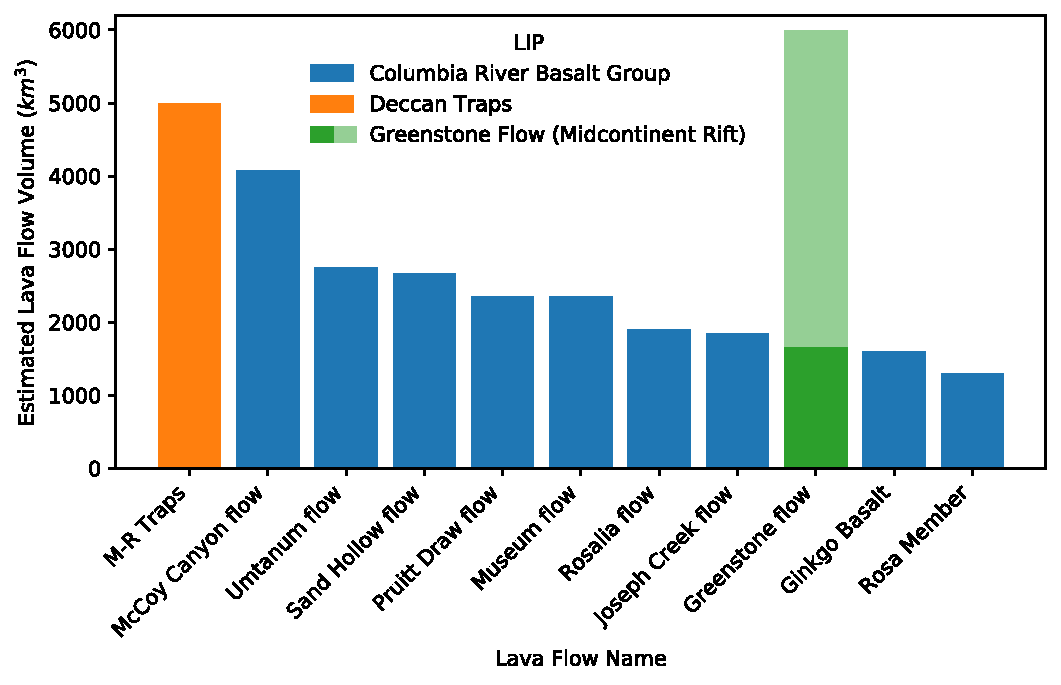
\includegraphics[width=\textwidth]{Figure/Lava_flow_rank.pdf}
\caption{\footnotesize{Bar plot of ten of the world's most voluminous single mafic lava flows currently known. With an estimated minimum volume of $\sim$1650 km$^3$ and likely volume as high as $\sim$6000 km$^3$, the Greenstone Flow from the 1.1 Ga Midcontinent Rift stands amongst the giant lava flows from the Deccan Traps and Columbia River basalts. M-R Traps = Mahabaleshwar–Rajahmundry lava flow in the Deccan Traps. Volume estimates from \citeA{Self2008a}, \citeA{Bryan2010a}, \citeA{Longo1984a}, and \citeA{Doyle2016a}.}}
\label{fig:lava_flow_rank}
\end{figure}

The Beaver Bay Complex, which sits stratigraphically above the Duluth Complex, is another intrusive complex that resulted from main stage magmatism. The exposed area of the Beaver Bay Complex is $\sim$1000 km\textsuperscript{2} where it has been mapped along the northwestern shore of Lake Superior in northeastern Minnesota (Fig. \ref{fig:Geologic_map}). The Beaver Bay Complex is a multi-phase, composite intrusive complex that intrudes parts of the NSVG (Fig. \ref{fig:Geologic_map}; \citeA{Miller1997a, Swanson-Hysell2020a}). Distinct from the deep plutonic intrusions of the Duluth Complex, the majority of the Beaver Bay Complex is formed of hypabyssal intrusions that were emplaced as dikes and sills at shallow depths \cite{Miller1997a}. Most of the Beaver Bay Complex intrusions are dioritic to gabbroic in composition \cite{Miller1997a}. The main lithology of the Beaver River diabase dikes and sills network within the Beaver Bay Complex is an ophitic olivine gabbro (Fig. \ref{fig:Field_photo}), but in wider areas of dikes and the upper parts of thick sills, this rock type can abruptly transition into intergranular olivine oxide gabbro, then into subprismatic (and commonly foliated) ferrogabbro, and finally into granophyric monzodiorite. The more evolved and later emplaced components of the Beaver River diabase network are commonly distinguished as the Silver Bay intrusions in the southern Beaver Bay Complex (Fig. \ref{fig:Geologic_map}). Overall being intermediate in composition, the Silver Bay intrusions lithologies range from ophitic olivine gabbro to ferrogranite \cite{Shank1989a}. Field mapping by \citeA{Miller1994a} found intrusive relationships between the Silver Bay intrusions and the Beaver River diabase. Angular inclusions of the host Beaver River diabase within marginal zones of the Silver Bay intrusions led \citeA{Miller1997a} to interpret that the Silver Bay intrusions intruded after the diabase crystallized.

One distinctive feature of the Beaver River diabase is its inclusions of anorthosite xenoliths. In the southern part of the Beaver Bay Complex, the Beaver River diabase occurs as dikes and sills, typically including anorthosites with various sizes ranging from centimeters to over 150 meters (Figs. \ref{fig:Geologic_map}, \ref{fig:Field_photo}; \citeA{Grout1939a, Morrison1983a}). The diabase in this region intrudes the Palisade rhyolite of the North Shore Volcanic Group (Fig. \ref{fig:Geologic_map}), which has a $^{206}$Pb/$^{238}$U date of 1093.94 $\pm$ 0.28 Ma (2$\sigma$ analytical uncertainty is presented for CA-ID-TIMS dates throughout this work; \citeA{Swanson-Hysell2019a}). The Beaver River diabase is locally intruded by the Silver Bay intrusions (Fig. \ref{fig:Geologic_map}). An aplite unit within the granophyre zone of one of these Silver Bay intrusions has a $^{206}$Pb/$^{238}$U date of 1091.61 $\pm$ 0.14 Ma \cite{Swanson-Hysell2019a}. Another arcuate, sill-like diabase body mapped as the Beaver River diabase outcrops along the eastern part of the complex (Fig. \ref{fig:Geologic_map}; \citeA{Miller1997a}). The diabase composition there is similar to that in the south and it also contains large anorthosite xenoliths with dimensions that exceed 100 meters at Carlton Peak (Fig. \ref{fig:Geologic_map}). The Beaver River diabase in the northern part of the complex, near the Houghtaling Creek area, typically forms narrow, near-vertical dikes instead of sheets in the southern and eastern regions (Fig. \ref{fig:Geologic_map}; \citeA{Miller1994a}). The diabase in this region only locally contains xenoliths of anorthosite. 

Hundreds of anorthosite xenoliths have been recognized and mapped within the Beaver River diabase (Fig. \ref{fig:Geologic_map}). Many hill tops in the Beaver Bay Complex, such as Carlton Peak and Britton Peak, are large anorthosite blocks (which lead \citeA{Lawson1893a} to erroneously conclude that they were relict Archean topography). Later work established the anorthosite blocks as xenoliths, which are now extensively documented through geologic mapping of the region (Fig. \ref{fig:Geologic_map}; \citeA{Miller2001a, Miller1988a, Miller1989a, Boerboom2004a, Boerboom2006a, Boerboom2006b, Boerboom2007a}) and outcrop-scale exposures (Fig. \ref{fig:Field_photo}). In the field, the anorthosites typically appear as subrounded to rounded, light-colored, translucent blocks that are in sharp contact with the hosting diabase (Fig. \ref{fig:Field_photo}). They also occur as exposures whose contact with the diabase is covered (Fig. \ref{fig:Field_photo}). \citeA{Grout1939a} suggested that the rounded anorthosites are the result of abrasion during transportation as they were entrained by the diabase (i.e. physical weathering within a magmatic system). While the Beaver River diabase is chilled against the North Shore Volcanic Group lithologies that it intrudes, the diabase is not chilled against the margin of the anorthosite xenoliths \cite{Morrison1983a, Miller1997a}. The lack of chilled contacts is consistent with the anorthosite being at elevated temperatures and cooling at the same time as the diabase magma (Fig. \ref{fig:thermal_history_model}).

The anorthosite xenoliths are dominantly monomineralic plagioclase that has an average anorthite content of $\sim$70\% \cite{Morrison1983a, Doyle2016a}. Interstitial pyroxene and olivine are present in minor concentrations in the xenoliths. Within the Carlton Peak anorthosite xenolith, up to 10 cm oikocrysts of olivine and pyroxene can occur. Nevertheless, the overall olivine content in the anorthosites is low. Interstitial titanomagnetite-ilmenite intergrowths that exceed 100 $\mu$m can be found with microscopy and $<$20 $\mu$m Fe-Ti oxide grains can be detected with scanning electron microscopy (Fig. \ref{fig:Field_photo}). Based on textural differences \citeA{Morrison1983a} divided the anorthosite xenoliths into four groups: one group which typically have well-developed granoblastic texture characterized by equigranular plagioclase crystals; another group which have interlocking, lath-shaped plagioclase crystals; an intermediate group which can have both granoblastic texture and interlocking plagioclase laths; and a brecciated group that have brittle deformation textures superposed on pre-existing textures. 

\subsection{Portage Lake Volcanics and the Greenstone Flow}

The Portage Lake Volcanics (PLV) is a $\sim$5 km thick, normally magnetized, dominantly olivine basalt to andesite volcanic succession that outcrops in northern Michigan (particularly along the Keweenaw Peninsula) as well as on Isle Royale (Fig. \ref{fig:Geologic_map}; \citeA{Huber1973a, Cannon2001a, Green1982a}). The Greenstone Flow of the Portage Lake Volcanic Group has been recognized as one of the largest lava flows on earth (Figs. \ref{fig:Geologic_map}, \ref{fig:lava_flow_rank}). It outcrops as the main ridge along the Keweenaw Peninsula and Isle Royale (Fig. \ref{fig:Geologic_map}). The flow can be correlated between the two outcrop regions on the basis of geochemical, petrographic, and paleomagnetic similarity of the flow itself and the flows above and below \cite{Longo1984a}. In both outcrop regions, the Greenstone Flow is underlain by conglomerate and overlain by pyroclastic breccia \cite{Lane1911a, Huber1973a}. On the Keweenaw Peninsula, the Greenstone Flow is exposed over 90 km with a range of thickness from $\sim$100 meters to a maximum thickness of over 450 meters, dipping to the northwest (Fig. \ref{fig:Geologic_map}; \citeA{White1960a}). On Isle Royale, the Greenstone Flow has a range of thickness from $\sim$30 meters to a maximum thickness of about 250 meters, dipping toward the southeast (Fig. \ref{fig:Geologic_map}; \citeA{Huber1973a}). More recently, \citeA{Doyle2016a} estimated that the total aerial extent of the Greenstone Flow could be up to $\sim$20000 km$^2$ by connecting it to the region of the Beaver Bay Complex. Taking thickness range of 100 to 300 meters, \citeA{Doyle2016a} estimated a total volume of 2000 to 6000 km$^3$. This volume range makes the Greenstone Flow one of the largest, if not the largest, single mafic lava flows on Earth (Fig. \ref{fig:lava_flow_rank}).

According to the mineralogical and textural attributes, the Greenstone Flow can be divided into four zones from bottom to top --- a lower ophitic zone, a ``pegmatoid'' or heterolithic zone, an upper ophitic zone, and an amygdaloidal zone \cite{Cornwall1951b}. The heterolithic zone contains lenses to layers of coarse-grained granophyric gabbro that are referred to in the literature as ``pegmatoid.'' Zircon crystallized in these layers have enabled the heterolithic zone to be targeted for U-Pb geochronology \cite{Davis1990a, Swanson-Hysell2019a}. A $^{206}$Pb/$^{238}$U zircon date of 1091.59 $\pm$ 0.27 Ma for the Greenstone Flow was developed from a sample from this zone in \citeA{Swanson-Hysell2019a}. The Greenstone Flow is typically interpreted to represent emplacement of a single body of magma that then underwent in situ differentiation \cite{Huber1973a, Davis1990a}. \citaA{Doyle2016a} favored a distinct model in which the Greenstone Flow is a composite unit, which they interpret to be indicated by lithologic zonation of ophitic basalt forming the upper and lower zones and an interior zone composed of prismatic ferrogabbro to granophyric monzodiorite. They envision emplacement of the Greenstone Flow started with voluminous eruption of olivine tholeiitic magma, forming the ophitic zones which while still crystallizing further inflated due to subsequent injection of a more evolved basaltic magma to form intergranular gabbro in the heterolithic zone. They considered this progression to be more consistent with observed abrupt lithologic changes from the ophitic zone to the heterolithic zone over centimeter to meter scales, inclusion relationships between evolved and ophitic Greenstone Flow lithologies, and remnant blocks of initially crystallized ophitic basalt interlayered with evolved lithologies within the heterolithic zone which contains the pegmatoids. In both the \citeA{Doyle2016a} model of multiple magma injections and the earlier models of in situ differentiation, it is migration of the most evolved and volatile-rich melts within the interior of the flow in the final stages of flow crystallization that led to the formation of some aplite dikes and the coarsest segregations containing granophyre. Both models also invoke a single basaltic parental magma with distinction of where differentiation occurred in fractionally crystallizing an evolving magma chamber or solely within a single, very thick flow.

\section{Methods and Results}

\subsection{Zircon Geochronology and Geochemistry}

A sample of an anorthosite xenolith within the Beaver River diabase was collected for U-Pb geochronology along Hwy 61 across from the Silver Bay taconite plant (MS99033; 91.26358\textdegree W 47.28888\textdegree N; Fig. \ref{fig:Geologic_map}). This sample comes from the same xenolith sampled for paleomagnetic study as site AX16 which has an exposed diameter of 27.5 meters (Fig. \ref{fig:Field_photo}). Thin sections were made from the geochronology sample as well as multiple paleomagnetic cores. As is shown in Fig. \ref{fig:Field_photo}F, plagioclase in this anorthosite xenolith have both equigranular crystals displaying a granoblastic texture and lath-shaped crystals displaying an interlocking texture. The occurrence of both textures is consistent with an interpretation that this anorthosite xenolith formed under elevated temperatures and experienced heating after initial crystallization. 

Zircons were separated from a kilogram of the anorthosite using common mineral separation methods (Supporting Information). The separated zircons were subhedral to anhedral crystals (z1-z4) and platy fragments (z5-z8). The subhedral to anhedral crystals are consistent with intercumulus crystallization within an adcumulate with platy fragments also being a common zircon morphology within anorthosites (e.g. sample AS3 of the Duluth Complex anorthositic series; \citeA{Schmitz2003a}). Eight chemically abraded zircons were analyzed by isotope dilution-thermal ionization mass spectrometry (ID-TIMS) in the Boise State Isotope Geology Laboratory using EARTHTIME tracer solutions \cite{Condon2015a}. Both zircon morphologies yield indistinguishable dates. Using six of these single grain dates (and excluding two due to interpreted Pb-loss) results in a weighted mean $^{206}$Pb/$^{238}$U date of 1091.83 $\pm$ 0.21/0.37/1.15 Ma (analytical/ analytical+tracer/ analytical+tracer+decay uncertainty; Fig. \ref{fig:BBC_geochron}). 

\begin{figure}
\noindent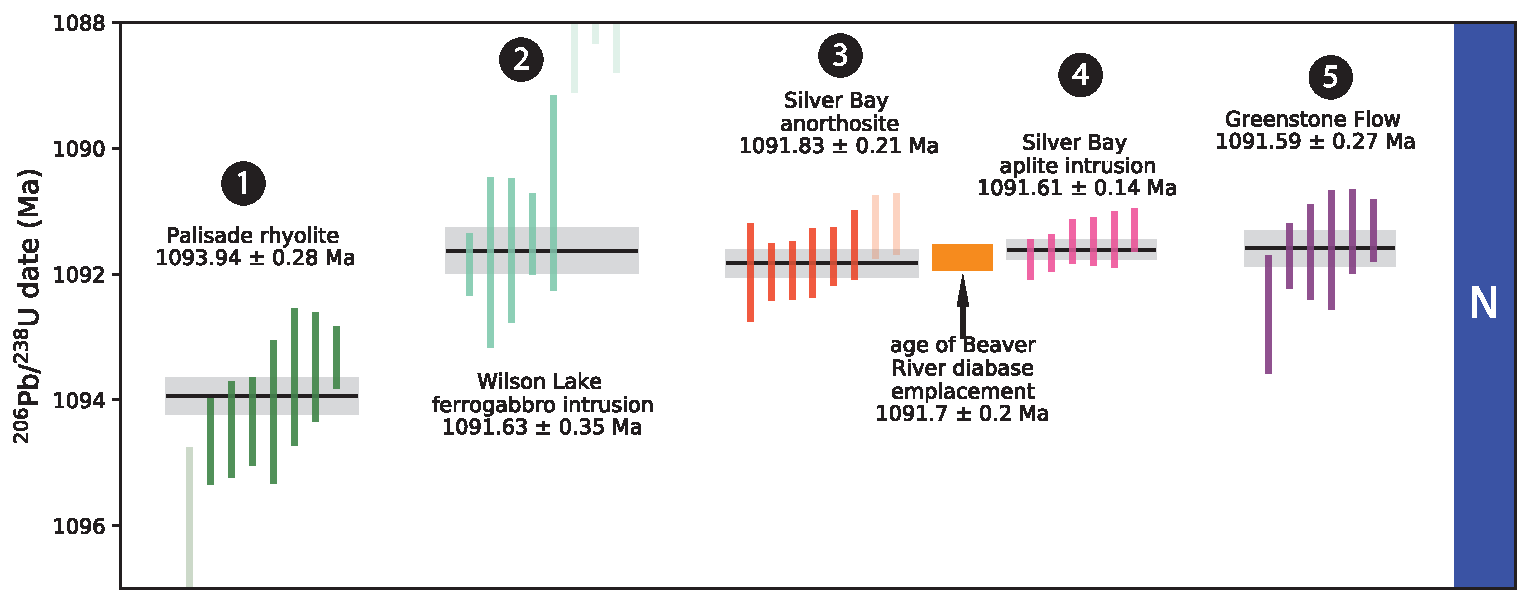
\includegraphics[width=\textwidth]{Figure/BBC_dates.pdf}
\caption{\footnotesize{New $^{206}$Pb/$^{238}$U zircon date of the anorthosite xenolith (dark orange) plotted in context of previously published $^{206}$Pb/$^{238}$U zircon dates from the North Shore Volcanic Group (NSVG) and other Beaver Bay Complex intrusions \cite{Swanson-Hysell2019a, Swanson-Hysell2020a}. These high-precision dates are consistent with field observations that the Beaver River diabase crosscuts the Palisade rhyolite (dark green) and is cut by the Silver Bay intrusions (pink). The estimated age of the Beaver River diabase from these constraints is shown by an orange box representing the 95$\%$ confidence interval. Each vertical bar corresponds to one $^{206}$Pb/$^{238}$U date from a single zircon crystal. The translucent bars represents zircons with interpreted Pb loss and are therefore not included in the weighted mean age calculations. Horizontal lines and gray boxes represent weighted mean $^{206}$Pb/$^{238}$U dates and their analytical uncertainty. The numbers of each geochronology sample correspond to those in Fig. \ref{fig:Geologic_map} where locations of these samples are shown.}}
\label{fig:BBC_geochron}
\end{figure}

This date provides a tight constraint on the age of the Beaver River diabase. Previously, the maximum age constraint for the Beaver River diabase came from the relationship that it cross-cuts the Palisade rhyolite of the North Shore Volcanic Group which has a $^{206}$Pb/$^{238}$U date of 1093.94 $\pm$ 0.28 Ma  \cite{Swanson-Hysell2019a}. With this new date, we know the crystallization age of the diabase to have been near-synchronous or younger than the date from the anorthosite xenolith. The Silver Bay intrusions, from which an aplite has a $^{206}$Pb/$^{238}$U date of 1091.61 $\pm$ 0.14 Ma, \cite{Fairchild2017a}, cross-cut the Beaver River diabase. These dates constrain the diabase to have been emplaced between 1091.83 $\pm$ 0.21 and 1091.61 $\pm$ 0.14 Ma (Fig. \ref{fig:BBC_geochron}). Assuming a uniform probability of diabase emplacement between the anorthosite and aplite dates and their normal distributed uncertainties, a 95\% confidence interval on the age of the diabase can be estimated by Monte Carlo simulation. This analysis gives an age for the diabase of 1091.7 $\pm$ 0.2 Ma (95\% CI). 

\begin{figure}[h!]
\noindent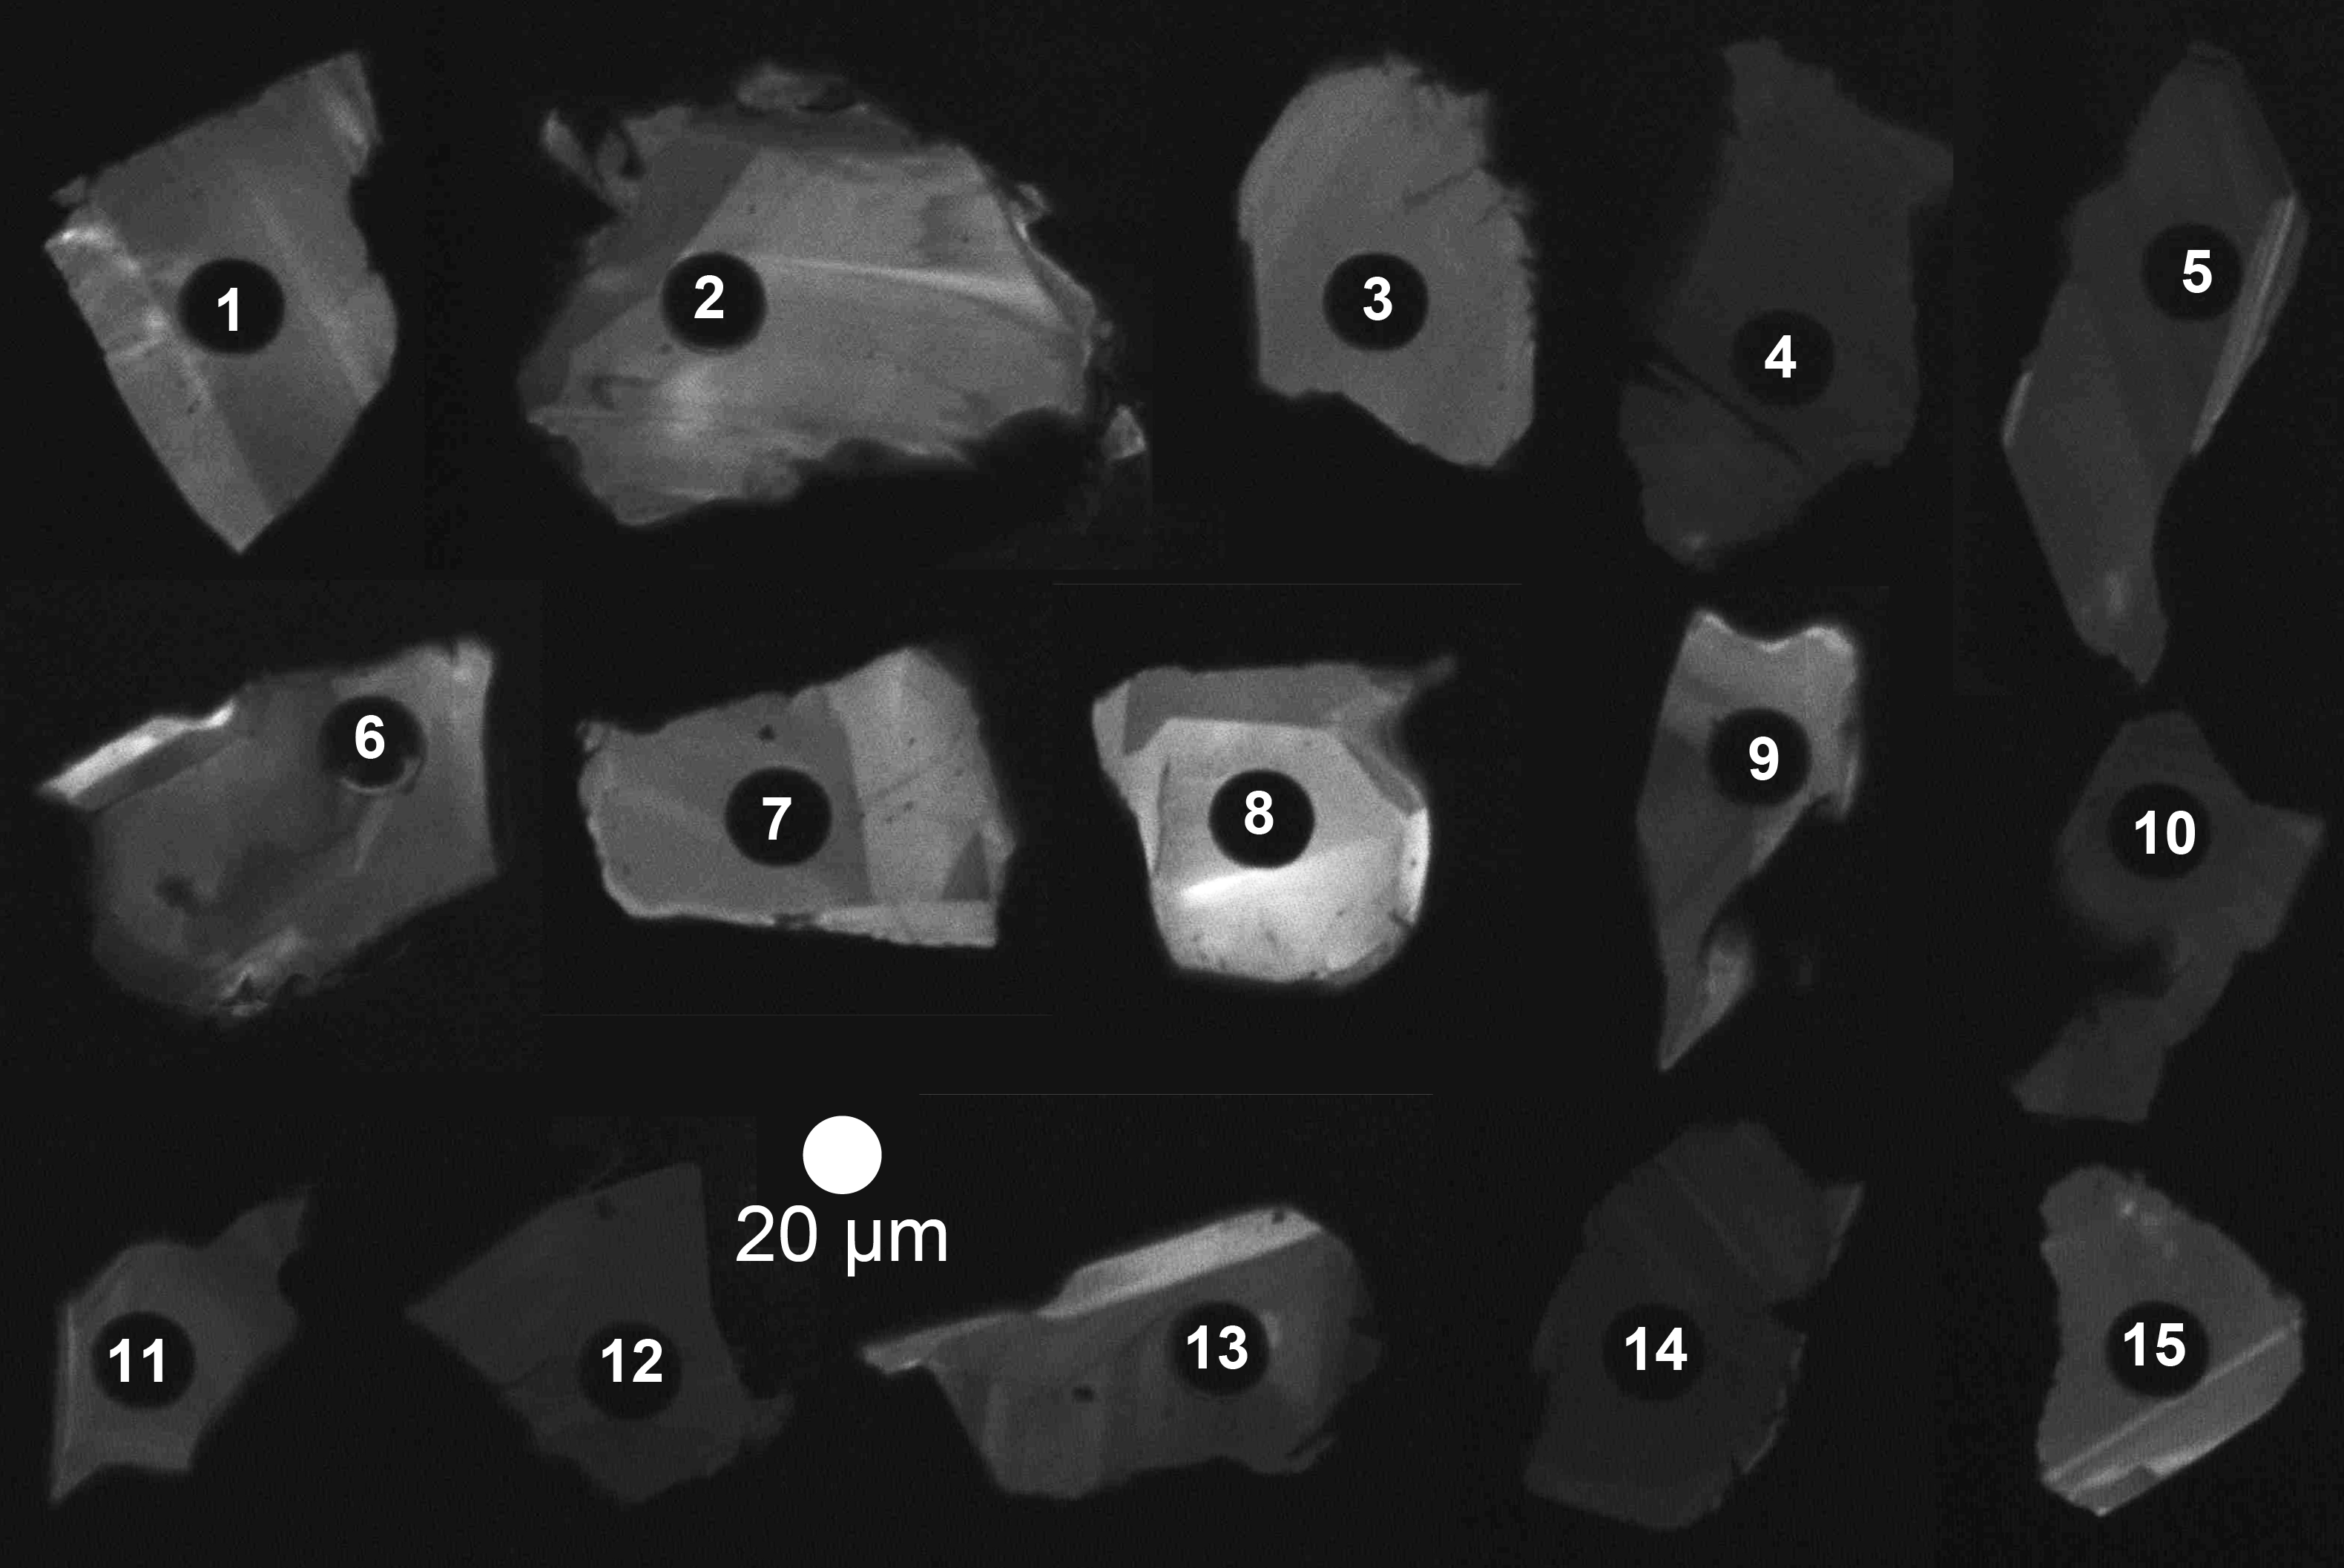
\includegraphics[width=\textwidth]{Figure/CL_montage.png}
\centering
\caption{\footnotesize{Cathodoluminescnece (CL) image montage of the 15 zircons laser-ablated for trace element analysis from sample MS99033. There are sharp boundaries between zones of differing CL response within many of the zircons attributable to variable REE concentrations. For example, the bright zoning in grain 15 has a thickness of $\sim$2 $\mu$m. Note that grain 1 (corresponding to spot 1) has a platy morphology, while the rest of the grains are subhedral to anhedral. }}
\label{fig:CL_image}
\end{figure}

\begin{figure}[h!]
\noindent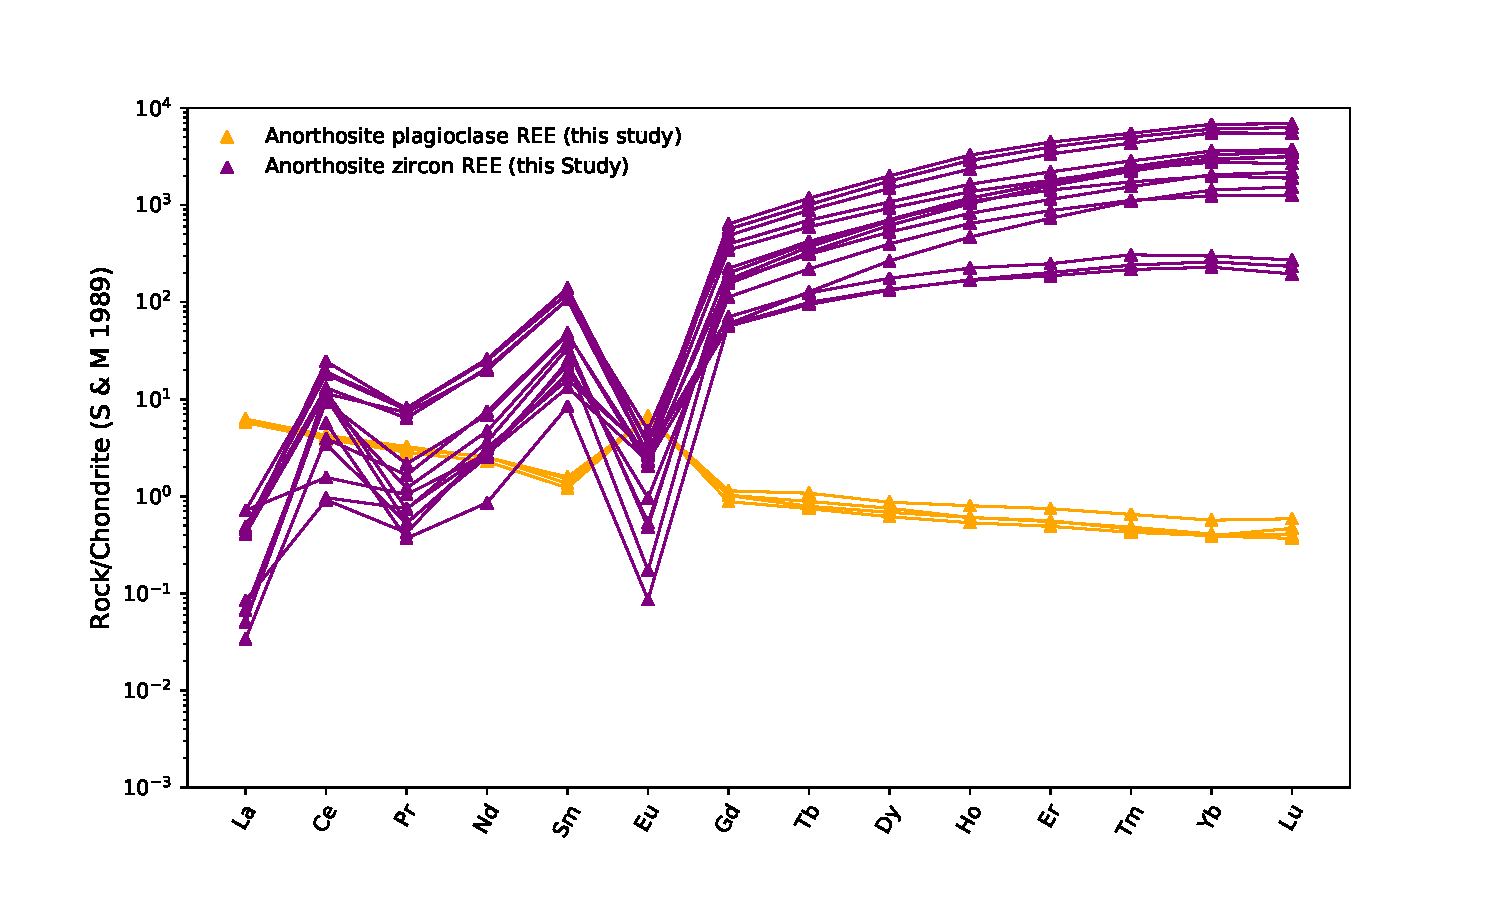
\includegraphics[width=\textwidth]{Figure/REE.pdf}
\centering
\caption{\footnotesize{Rare earth element (REE) analyses for plagioclase crystals from anorthosite xenoliths and for 15 zircons from geochronology sample MS99033 (anorthosite xenolith site AX16) developed by inductively coupled plasma mass spectrometry. All data are chrondrite-normalized \cite{Sun1989a}.}}
\label{fig:REE}
\end{figure}

An additional 15 zircons were characterized using cathodoluminescence (CL) imaging and laser ablation-inductively coupled plasma mass spectrometry (LA-ICPMS), with methods and instrumentation described in the Supporting Information. CL images reveal internal planar zones of variable brightness, often with darker interior zones and outer brighter zones (Fig. \ref{fig:CL_image}). All crystals exhibit sharp, micron-scale transitions between zones, and LA-ICPMS analyses quantify CL brightness as correlated with rare earth elements (REE) content. REE patterns in zircons exhibit a significant chondrite-normalized negative Eu anomaly (Fig. \ref{fig:REE}). The Ti-in-zircon thermometer gives a range of estimated zircon crystallization temperatures from 998\textdegree C to 860\textdegree C with a mean of $\sim$950\textdegree C (\citeA{Ferry2007a}; Supporting Information). Decreasing temperatures are correlated with deepening of the negative Eu anomaly and increasing incompatible trace element (e.g. Hf, Th) incorporation into zircon. These data are consistent with a model of magmatic zircon crystallizing from cooling and fractionating interstitial residual melt within the cumulate plagioclase framework.

\subsection{Paleomagnetism}

We collected paleomagnetic cores that are 2.5 cm in diameter along the southern and eastern Beaver Bay Complex with a particular focus on acquiring paired sites of anorthosite xenoliths and their local diabase hosts. Sample cores were collected using a hand-held gasoline-powered drill and were oriented using a magnetic compass as well as a sun compass when possible. Sun compass orientations were preferentially used for determining the sample azimuth. Typically, 7-10 cores were collected for each anorthosite xenolith and their diabase hosts. A total of 17 diabase and 22 anorthosite sites were sampled (Table \ref{tab:Pmag_site_data}). A table that summarizes the measured dimensions of each anorthosite xenolith sampled and the distance between each anorthosite paleomagnetic site and closest diabase host site is provided in the Supporting Information.  

Samples underwent step-wise demagnetization and analyses in the magnetically-shielded room at the UC Berkeley Paleomagnetism Lab. 7 sites from the Beaver River diabase underwent alternating field (AF) demagnetization with peak fields from 1 mT to 130 mT. An ASC TD-48SC thermal demagnetizer was used to demagnetize 10 diabase sites and all 22 anorthosite sites in a step-wise manner, with reduced step increments between 540\textdegree C and 585\textdegree C. The typical magnetic field inside the shielded room is $<$500 nT and the field inside the thermal demagnetizer chamber is $<$10 nT. The quartz glass sample rod of the UC Berkeley system is typically measured at 5 $\times$ 10$^{-12}$ Am$^{2}$. All remanence measurements were made on a 2G Enterprises DC-SQUID superconducting rock magnetometer equipped with inline AF coils and an automated sample changer system. The PmagPy software package was used to implement least-square fits to specimen demagnetization data \cite{Tauxe2016a}. Measurement level data are available within the MagIC database (\url{https://earthref.org/MagIC/17102/400e0fb3-a79b-42bd-aeab-9005d2e3b438}; UPDATE ONCE PUBLICATION DOI IS GENERATED)

\begin{figure}
\noindent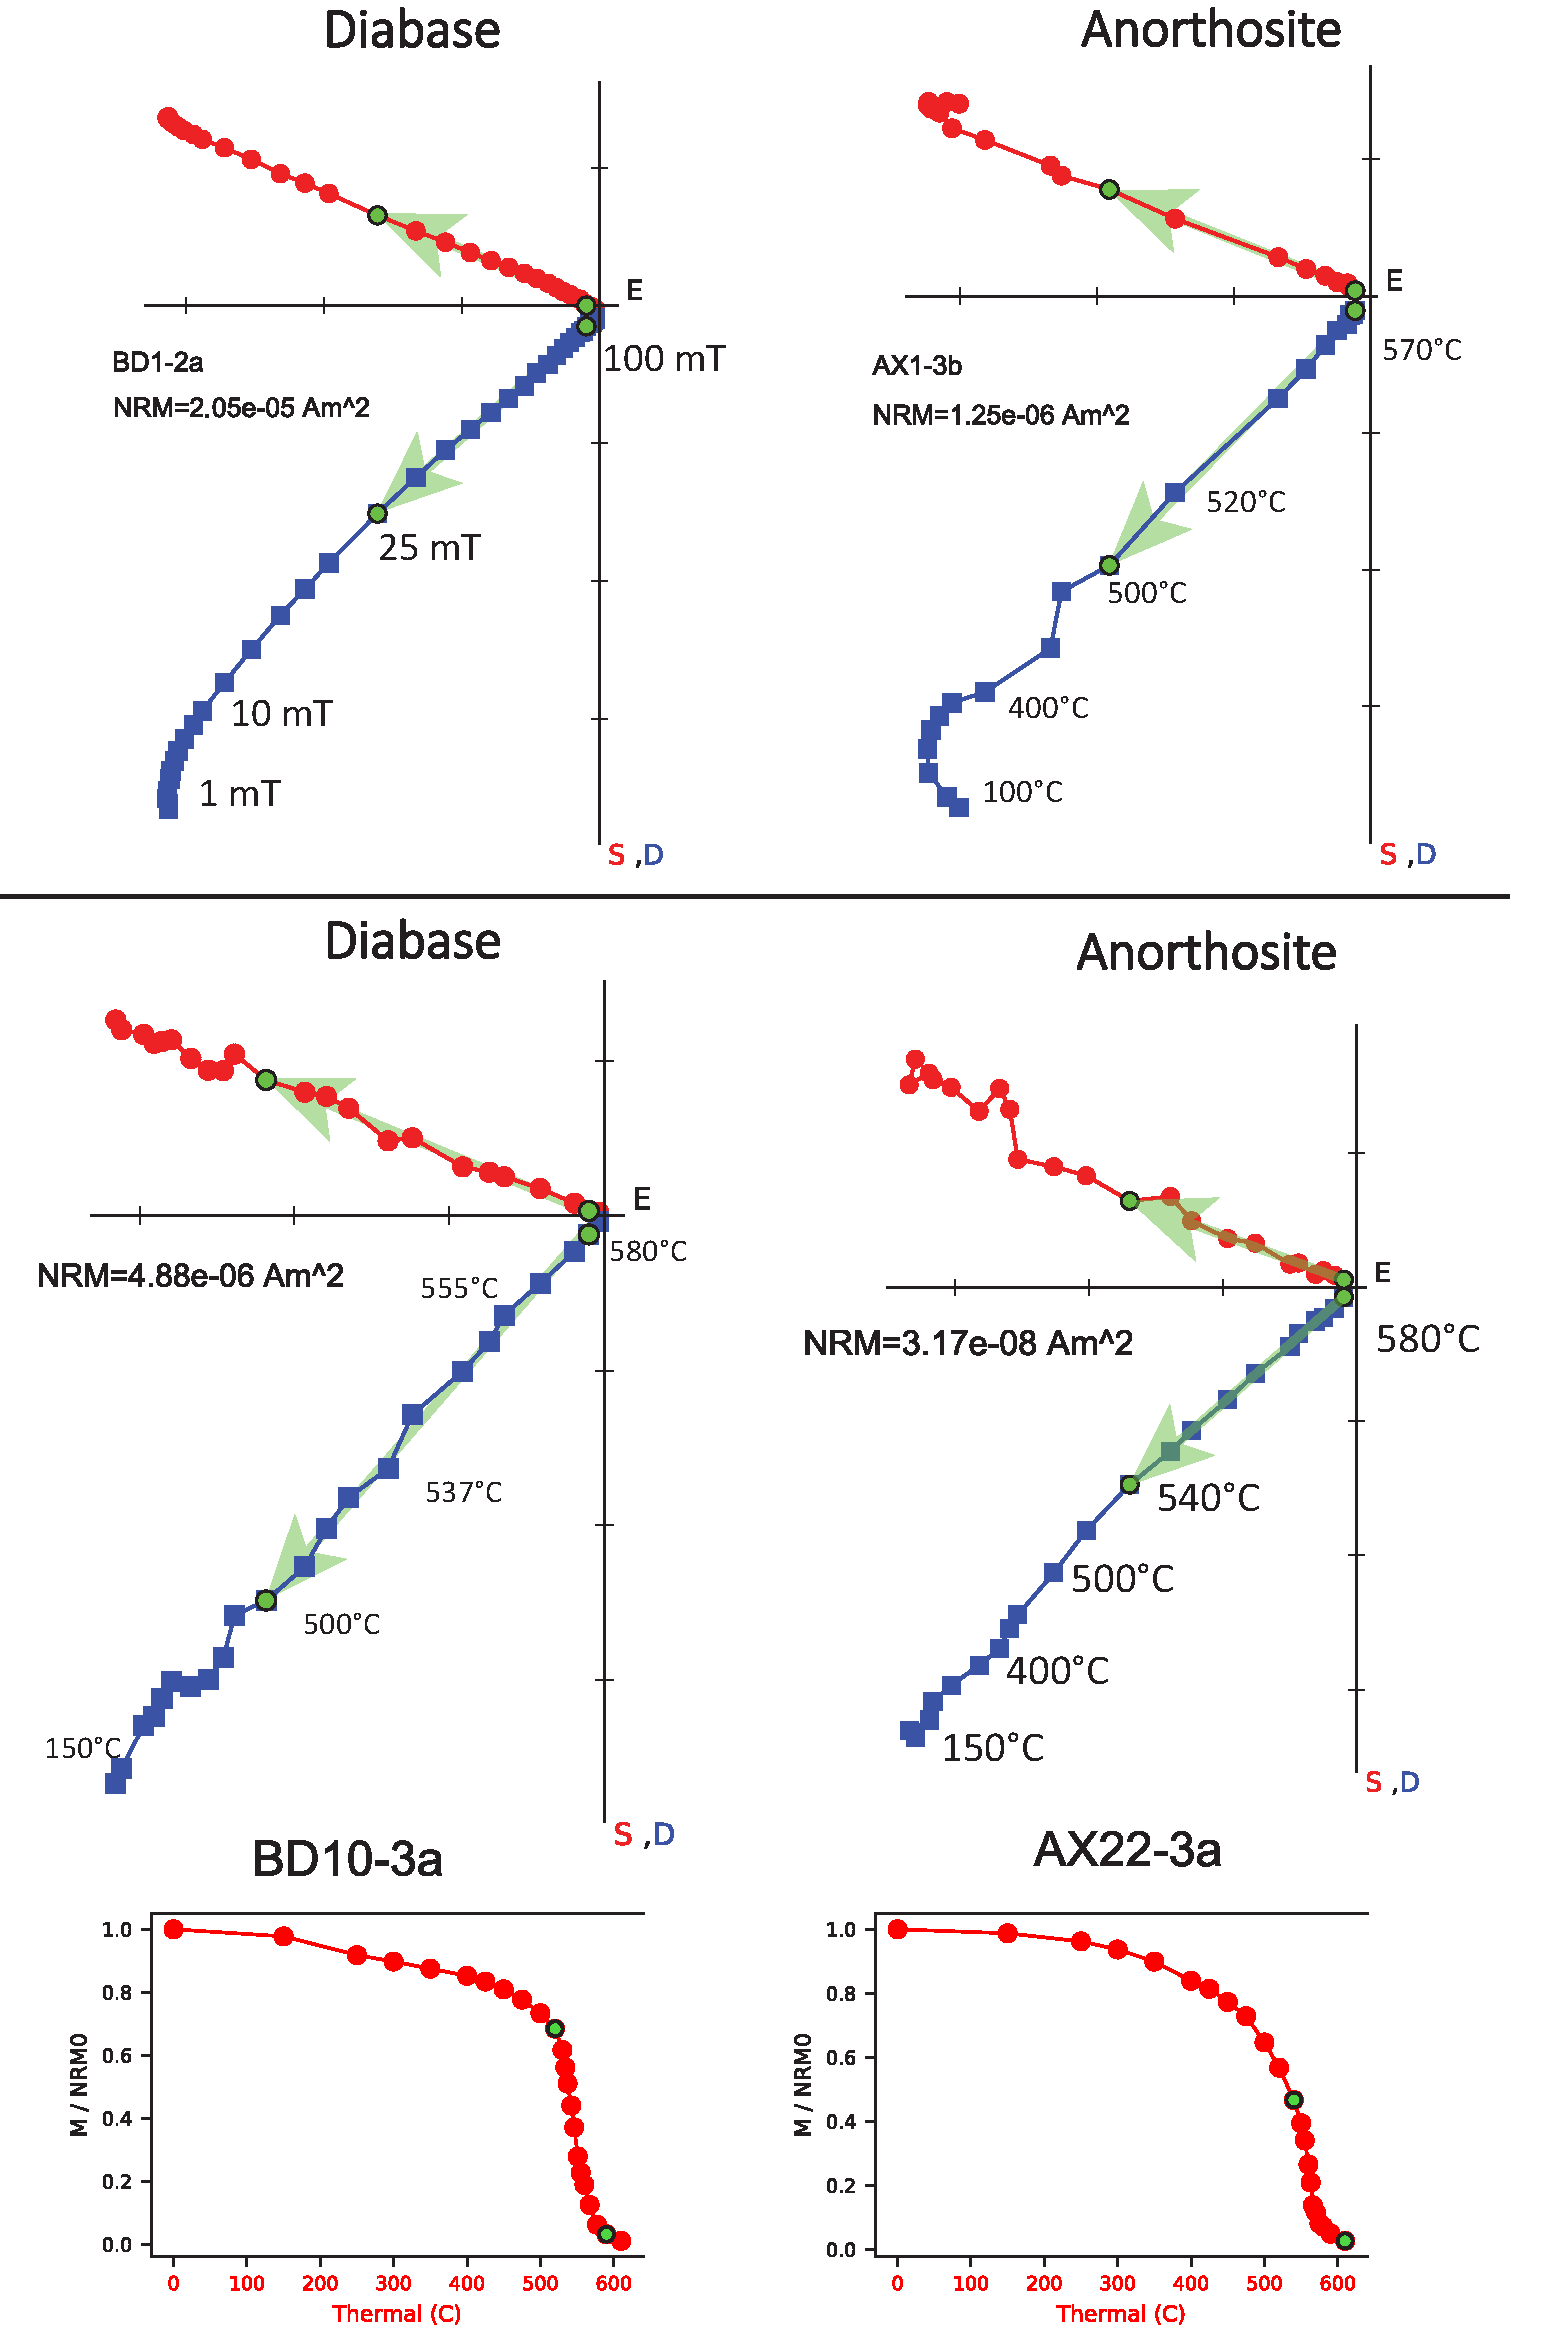
\includegraphics[width=\textwidth]{Figure/Demag.pdf}
\caption{\small{Example orthogonal vector demagnetization diagrams for diabase and anorthosite specimens. Anorthosite site AX1 is a xenolith within the diabase sampled as BD1. Similarly, AX22 is from a xenolith within the BD10 diabase. Both AF and thermal demagnetization show dominantly univectoral decay of characteristic remanent magnetizations (ChRM) toward the origin after removal of minimal secondary components. The data show very similar ChRM directions between the paired diabase and anorthosite xenoliths sites. Representative magnetization intensity versus thermal demagnetization step plots are paired with orthogonal vector plots for specimen BD10-3a and AX22-3a.}}
\label{fig:Demag}
\end{figure}

For both the diabase and anorthosite demagnetization, principal component analyses show that an origin trending characteristic remanent magnetization (ChRM) can be isolated after the removal of a minimal secondary component during the first few low coercivity ($<$10 mT) or low temperature ($<$200\textdegree C) demagnetization steps (Fig. \ref{fig:Demag}). The ChRMs typically unblock through thermal demagnetization steps from $\sim$500\textdegree C to $\sim$580\textdegree C, consistent with the component being held by low-titanium titanomagnetite. We interpret this component as a primary remanent magnetization acquired during the emplacement and cooling of the Beaver River diabase.

The site mean paleomagnetic directions are shown in Table \ref{tab:Pmag_site_data}. We present both AF and thermal demagnetization results for the Beaver River diabase as both methods are effective in removing the secondary components and isolating the coherent and univectoral ChRM. Based on specimen and site level demagnetization behavior and the proximity between paired paleomagnetic sites of the anorthosite xenoliths and the diabase, we grouped the anorthosite xenoliths and their diabase hosts into individual cooling units and calculated a paleomagnetic pole position from the mean of the cooling unit virtual geomagnetic poles (Fig. \ref{fig:Direction_pairs}). 

\begin{figure}
\noindent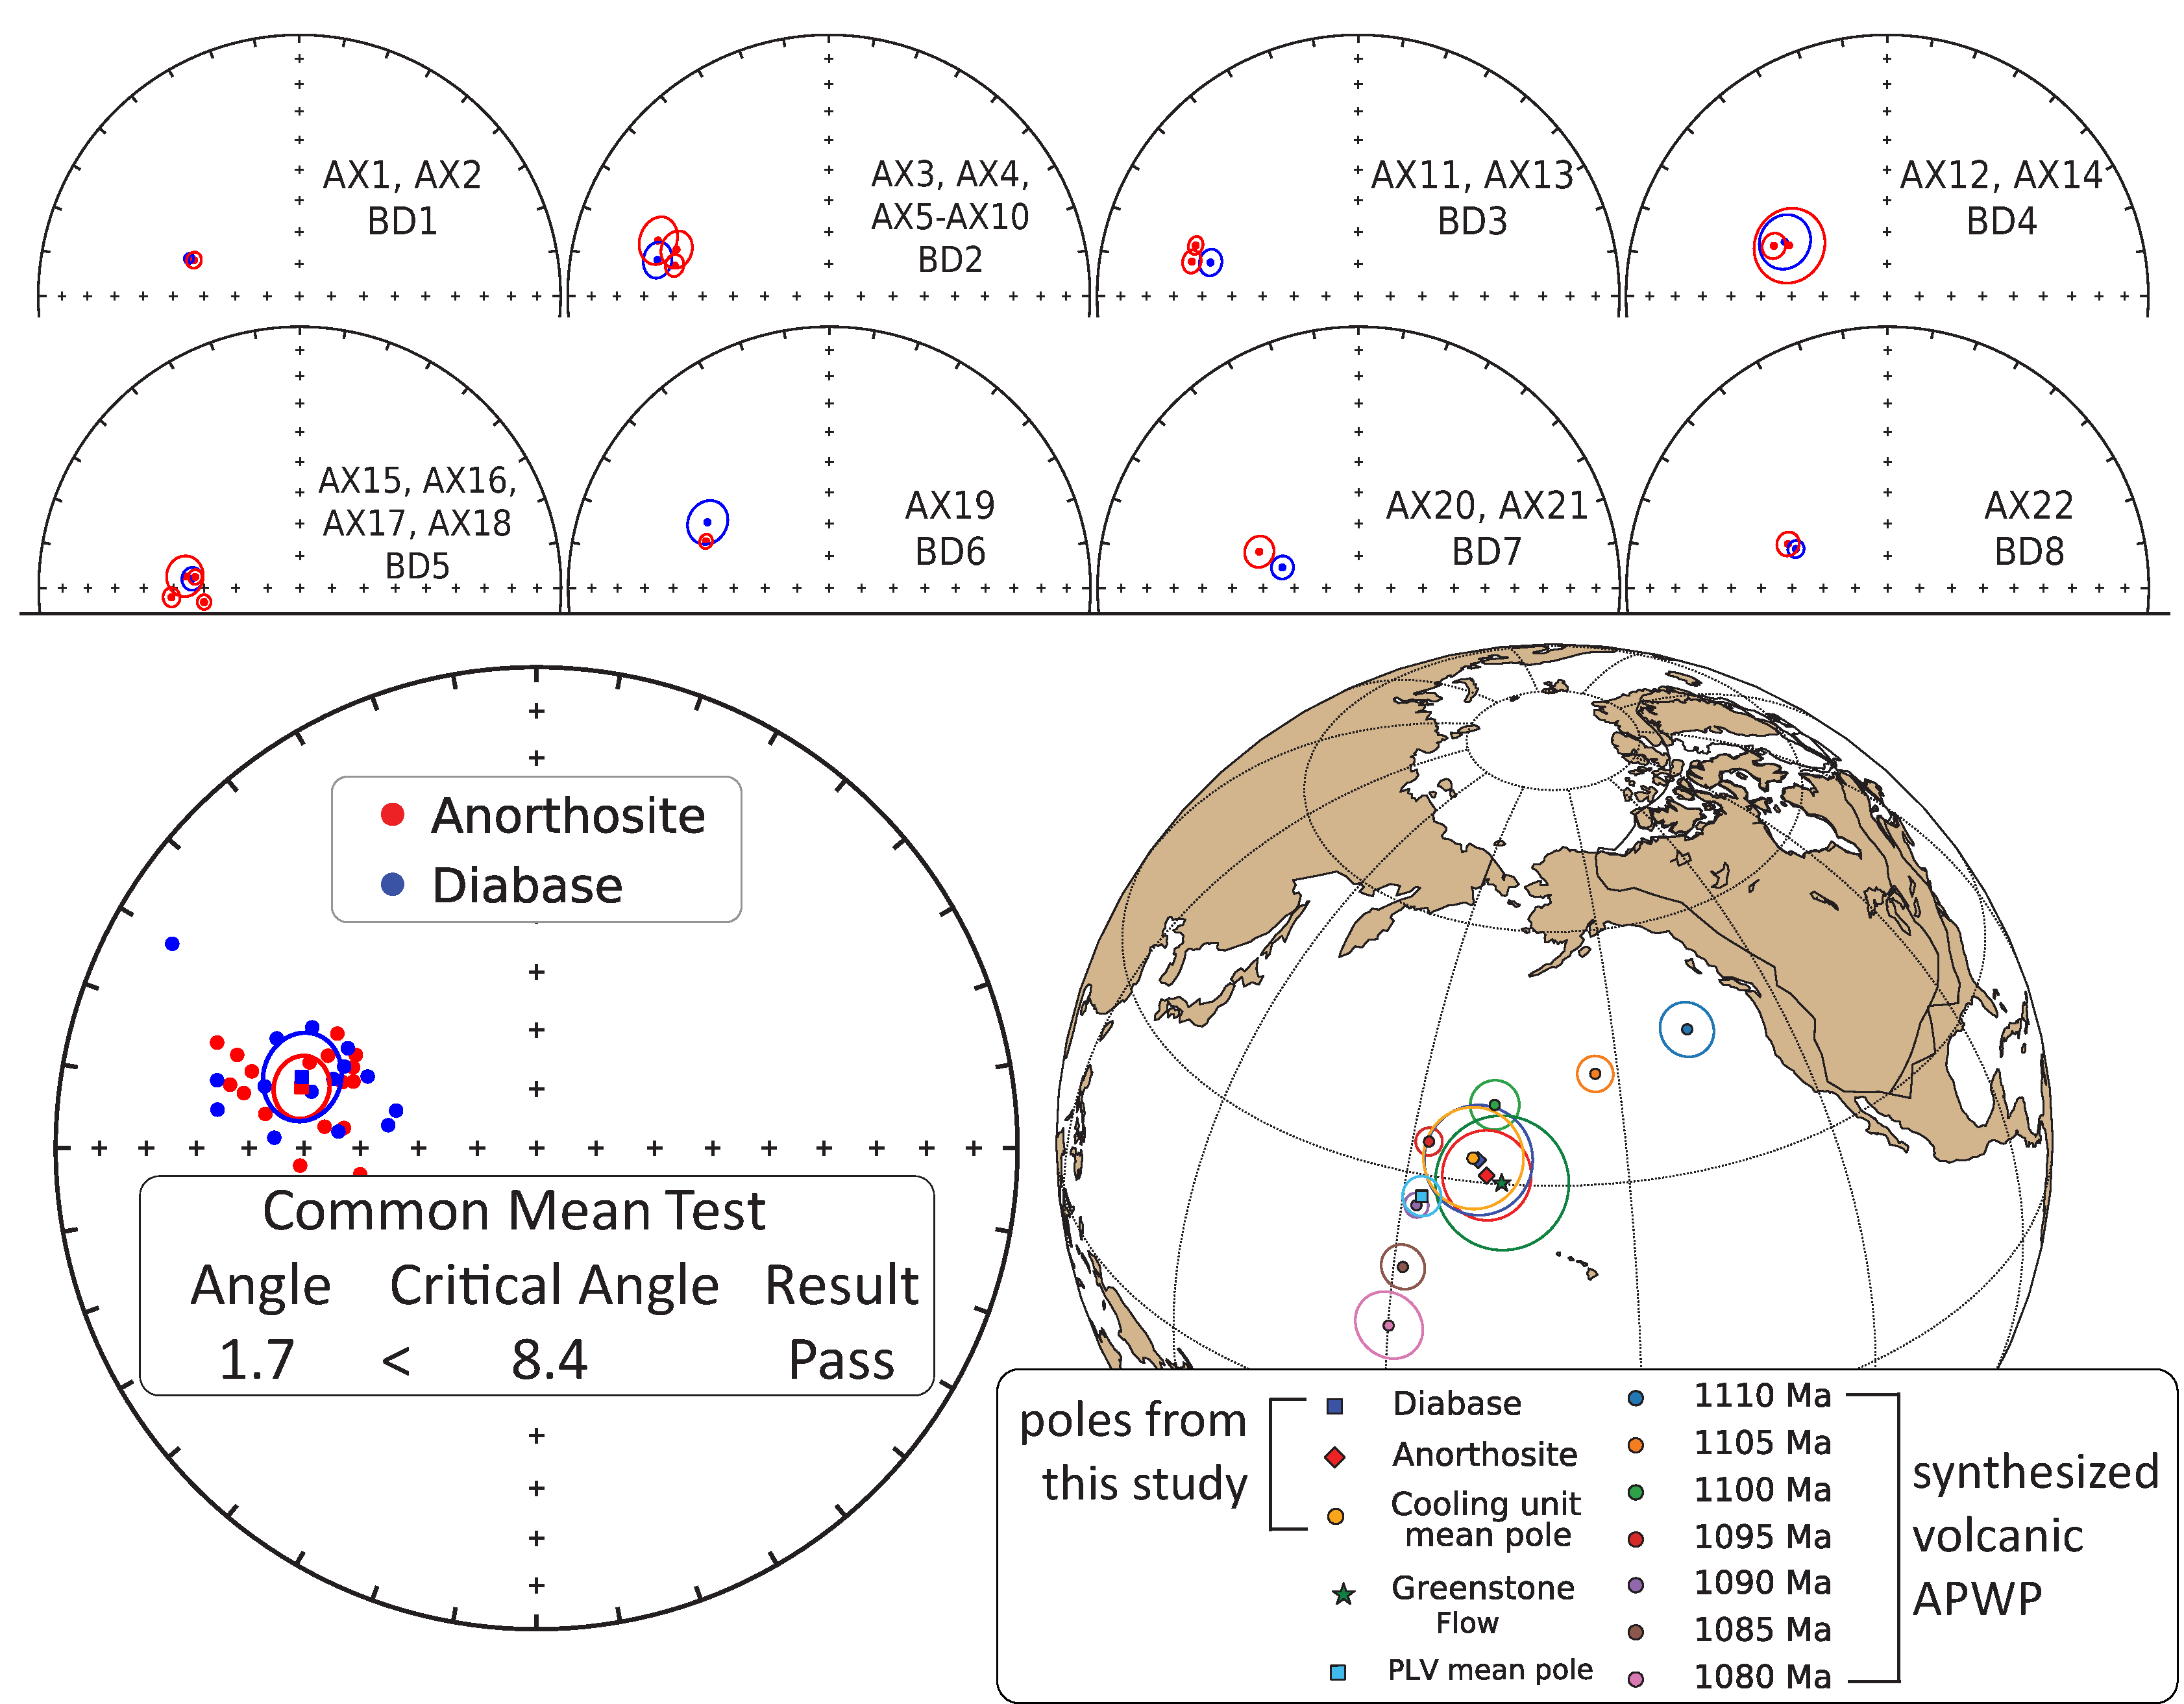
\includegraphics[width=\textwidth]{Figure/Direction_pairs.pdf}
\caption{\small{Top: Equal area plots of paleomagnetic directions from the anorthosite xenoliths and their local diabase hosts. AX: anorthosite xenolith site; BD: Beaver River diabase site. Bottom: Site mean paleomagnetic directions from the Beaver River diabase and anorthosite xenoliths are plotted on equal area plots. The anorthosite and diabase sites share a common mean as summarized by the results of the \citeA{McFadden1990a} common mean test. Mean paleomagnetic pole positions of all diabase sites, all anorthosite sites, as well as a grand mean pole developed by grouping the anorthosite and diabase sites into individual cooling units are plotted against a synthesized Laurentia APWP based on poles from Midcontinent Rift volcanics and sedimentary rocks \cite{Swanson-Hysell2019a}. The paleomagnetic poles from the diabase and anorthosite are indistinguishable with the Greenstone Flow pole developed by \citeA{Foucher2018a}, but they all are distinct from the Portage Lake Volcanics mean pole \cite{Swanson-Hysell2019a}. All directions shown are tilt corrected.}}
\label{fig:Direction_pairs}
\end{figure}

Tilt-correcting the paleomagnetic directions to paleohorizontal is necessary for developing accurate paleomagnetic poles from the diabase and the anorthosite xenoliths to be compared to the Keweenawan Track apparent polar wander path (APWP; Fig. \ref{fig:Direction_pairs}, \citeA{Swanson-Hysell2019a}). For intrusive igneous rocks, tilt corrections can be difficult to constrain due to the lack of a clear paleohorizontal reference. Many paleomagnetic studies of Midcontinent Rift intrusive rocks in the Lake Superior region did not apply tilt corrections to their data \cite<e.g.,>{Beck1969a, Beck1970a, Books1966a}. However, we can determine the structural orientation of the Beaver River diabase using the abundant igneous fabric orientations measured on the diabase as well as bedding orientations measured from adjacent volcanic units \cite{Boerboom2004a, Boerboom2006a, Boerboom2006b, Boerboom2007a, Miller2001a}. We compile the igneous layering measurements from the Beaver River diabase and the volcanic bedding orientations from the Schroeder-Lutsen basalt which is overlying the Beaver Bay Complex (Fig. \ref{fig:Geologic_map}). Despite the uncertainties associated with using igneous fabrics orientations as paleohorizontal references, the mean tilt orientations of the fabrics of the Beaver River diabase and the volcanic bedding orientations of the Schroeder-Lutsen basalt are similar (diabase overall dip direction - dip: 128.5 - 10.2; basalt dip direction - dip: 142.2 - 13.6). We combine the structural measurements from the Beaver River diabase and the Schroeder-Lutsen basalt and derived two sets of tilt corrections for the paleomagnetic directions of the diabase and anorthosite (dip direction - dip in the southern Beaver Bay complex: 128.7 - 12.9; in the eastern Beaver Bay Complex: 145.6-13.1, Supporting Information). The advantage of using the structural orientations from the Schroeder-Lutsen basalt is that the arcuate shape of the Beaver River diabase intrusions is nicely captured by the variation of lava dip directions while the dip angles of the basalt and diabase are very similar (Fig. \ref{fig:Geologic_map}).

The tilt-corrected ChRMs in both lithologies are west-northwest and down, yielding good specimen-level and site-level consistency (Figs. \ref{fig:Demag} and \ref{fig:Direction_pairs}). Close directional similarities between each anorthosite xenolith and their host diabase are supported by 9 out of a total of 17 diabase-anorthosite paleomagnetic site pairs passing a common mean test \cite{McFadden1990a}. The overall mean directions between the two lithologies are indistinguishable as they also pass a common mean test (Fig. \ref{fig:Direction_pairs}, \citeA{McFadden1990a}). For the anorthosite sites that do not pass a common mean test with their diabase hosts, they nevertheless have coherent specimen-level directions that are close to their host diabase directions (Fig. \ref{fig:Direction_pairs}). We also plot the tilt-corrected mean pole of sites from both lithologies (diabase: 32.5\textdegree N, 189.5\textdegree E, N = 15, A95 = 6.3, k = 37.4; anorthosite: 30.9\textdegree N, 190.8\textdegree E, N = 17, A95: 5.2, k = 48.5; Table. \ref{tab:Pmag_site_data}) in context of a previously synthesized APWP from the volcanics of the Midcontinent Rift \cite{Swanson-Hysell2019a} and show the poles to lie near the expected 1090 Ma and 1095 Ma pole positions (Fig. \ref{fig:Direction_pairs}). The mean pole position of the interpreted cooling units (32.7\textdegree N, 188.8\textdegree E, N = 15, A95 = 5.9, k = 41) lies close to the mean pole position derived from the \textit{ca.} 1092 Ma Portage Lake Volcanics (Fig. \ref{fig:Direction_pairs}), consistent with the coeval magmatic activity between the Beaver River diabase and the Portage Lake Volcanics. If it is included in future Laurentia APWP compilations, it is this cooling unit mean pole paired with the estimated diabase emplacement age of 1091.7 $\pm$ 0.2 Ma that should be used.

\subsection{Thermal history model}

\begin{figure}
\noindent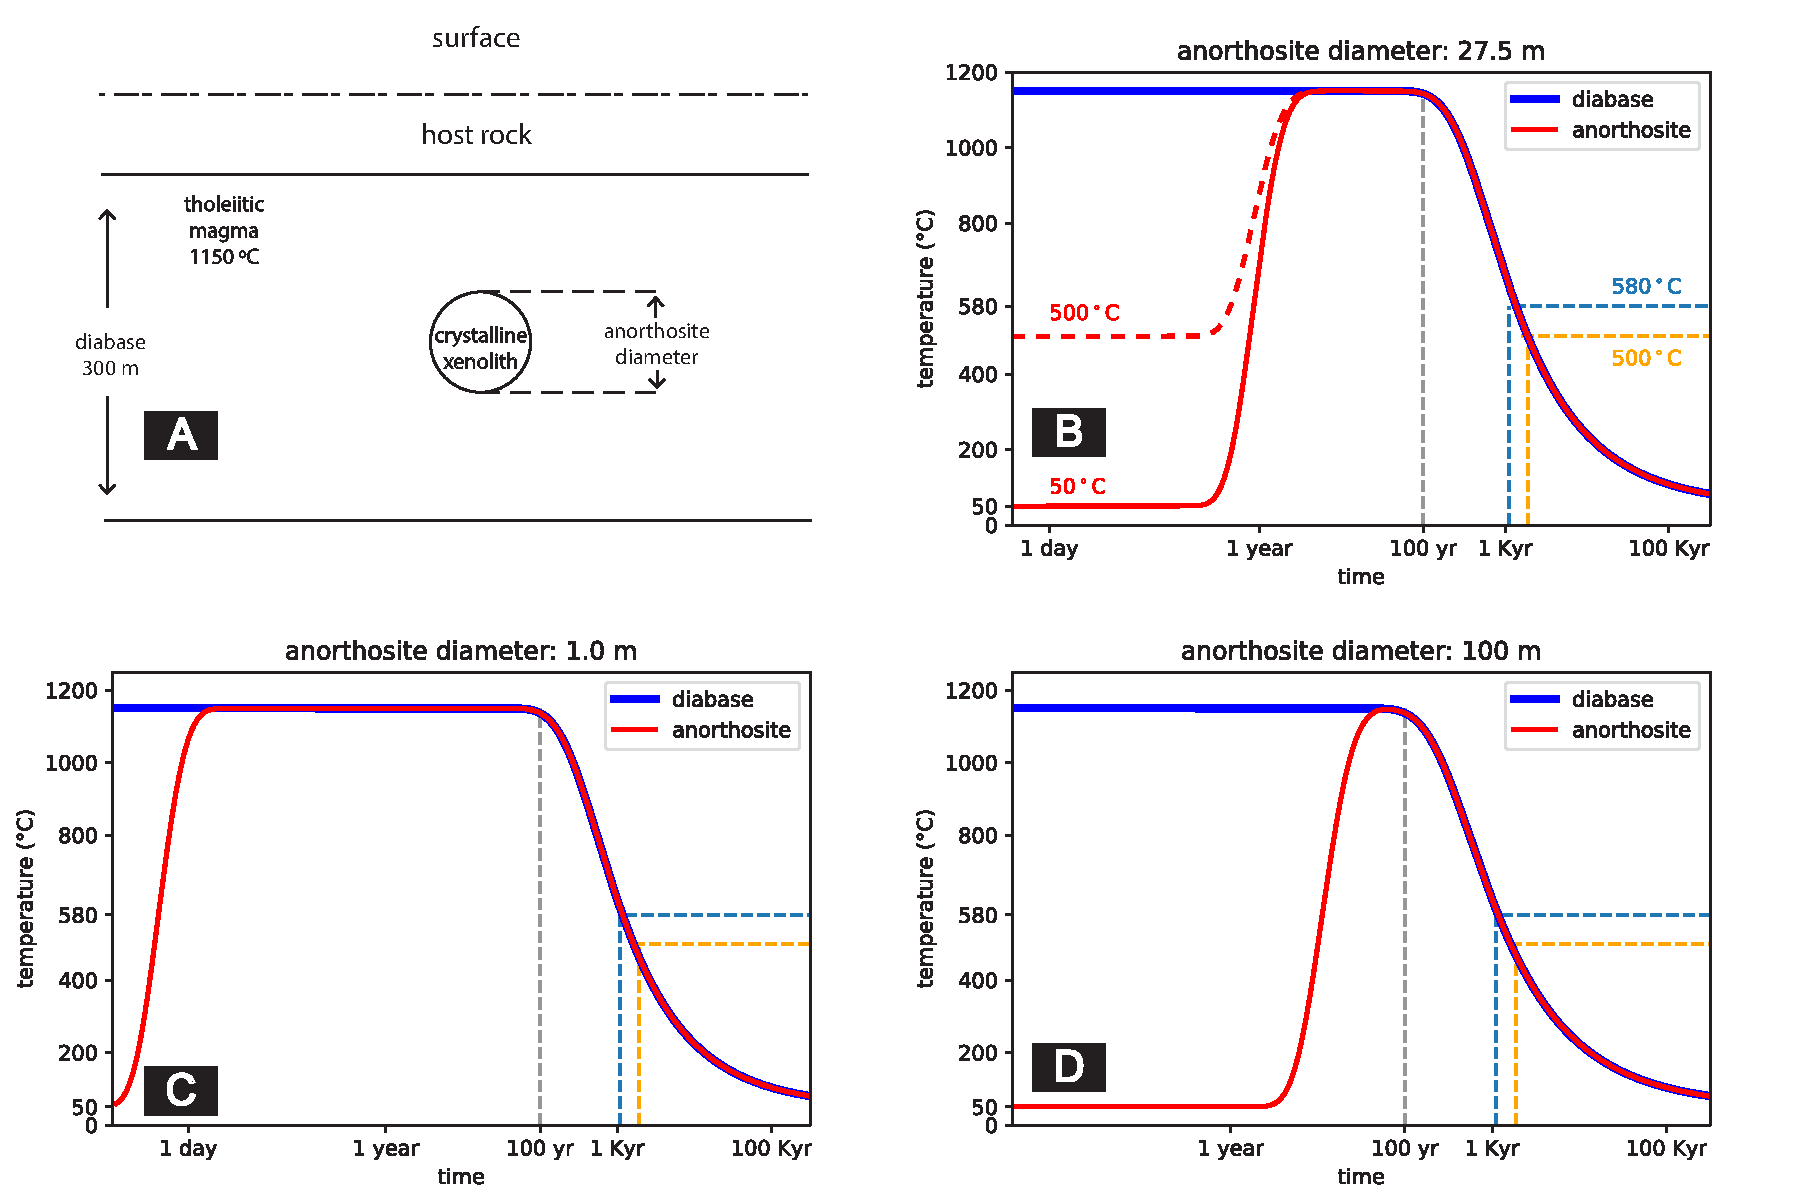
\includegraphics[width=\textwidth]{Figure/thermal_history_model.pdf}
\caption{\footnotesize{Thermal history model of the Beaver River diabase and its anorthosite xenoliths after emplacement at hypabyssal depths. (A) Schematic diagram for the thermal model considering cool anorthosite xenoliths as crystalline spheres residing in the middle of a diabase sill. Together they are hosted by cool country rocks at shallow depths. (B) Specific model for anorthosite AX16 (diameter of 27.5 meters) within its diabase sill host which is estimated to be 323 meters thick. (C) Thermal history model considering an anorthosite xenolith 1 meter in diameter residing in a 300 meter diabase sill. (D) Thermal history model considering an anorthosite xenolith 100 meter in diameter residing in a 300 meter diabase sill. These models show that anorthosite xenoliths were heated up to the diabase melt temperature after the emplacement, regardless of size. The time elapsed between at magnetite blocking temperatures (580\textdegree C and 500\textdegree C) during cooling is on the scale of a thousand years.}}
\label{fig:thermal_history_model}
\end{figure}

The consistency of the paleomagnetic directions between the anorthosite xenoliths and the host diabase indicate that the anorthosites were heated above the Curie temperature of low-titanium titanomagnetite ($\sim$580\textdegree C) within the Beaver River diabase. To determine whether this thermal history is consistent with the geometry of the units and to gain more insight into the emplacement history of the xenoliths, we developed a cooling model. In this model, the anorthosite xenoliths are considered to be solid spheres with an initial cool temperature embedded in a uniform sheet of diabase magma \cite{Delaney1987a, Unsworth1979a}. The modeled thermal histories for various sizes of anorthosite xenoliths are shown in Fig. \ref{fig:thermal_history_model}. In one end member case, the initial temperature of the anorthosites is assumed to be 50\textdegree C. While this temperature is unrealistically low given that the anorthosites likely have a deep crustal source, thermal modeling shows that even a 100-meter anorthosite xenolith with such low initial temperature would have been heated to the temperature of the tholeiitic magma (1150\textdegree C) within the sill. This temperature is well above the Curie temperature of magnetite. Anorthosite xenoliths with an assumed initial temperature of 500\textdegree C will equilibrate with the magma temperature on a similar, but slightly shorter, timescale. Therefore, the model predicts that the remanent magnetizations of the anorthosites will be reset during emplacement within the diabase sills, regardless of their initial temperatures. Model parameters set to match the xenolith AX16, from which a U-Pb date was developed in this study, leads to a model where the 27.5 m xenolith would have stayed at the magma temperature for about 100 years after sill emplacement (Fig. \ref{fig:thermal_history_model}). This duration estimate is a minimum as it does not consider heating associated with melt in the lower crust or during ascent prior to emplacement although this was likely rapid. The xenolith would have then cooled through the Curie temperature of magnetite (580\textdegree) after $\sim$1 kyr and acquired its magnetization as it cooled through magnetite blocking temperatures (down to $\sim$500\textdegree, Fig \ref{fig:Demag}).

\section{Discussion}
\subsection{Origin and Age of the Anorthosite Xenoliths}

There have been divergent interpretations regarding the age and magma source of the anorthosite xenoliths in the Beaver River diabase (Fig. \ref{fig:Geologic_map}). \citeA{Grout1939a} recognized the xenolithic nature of the anorthosites and suggested that the massive intrusion of the older anorthositic gabbro within the Duluth Complex may have supplied anorthosite fragments that were later entrained by the Beaver River diabase emplacement. \citeA{Morrison1983a}, on the other hand, argued that the xenoliths were sourced from Paleoproterozoic or Archean lower crust that were liberated and contaminated by Midcontinent Rift magmas based on Sm and Nd isotopic data. They interpreted a Sm-Nd model age of 1.9 Ga from one of the xenoliths as providing a minimum crystallization age for the anorthosites though they acknowledged that these constraints are not definitive with respect to the age. 

In contrast to this Archean to Paleoproterozoic model, \citeA{Miller1997a} favored a scenario where the anorthosite crystallized as part of Midcontinent Rift magmatism. They cited work by \citeA{Kushiro1980a} who showed that the changing density contrast between labradoritic to bytownitic plagioclase and tholeiitic magma at different crustal pressures would promote flotation of plagioclase in deep ($>$20 km) crustal magma chambers and the creation of anorthosite cumulates in the lower crust. This mechanism of plagioclase flotation likely created massive anorthosite cumulates in the roof zones of subcrustal magma chambers during MCR magmatism. \citeA{Miller1990a} speculated that plagioclase-phyric magmas tapped from these deep chambers fed shallow ($\sim$5 km) subvolcanic intrusions of the Duluth Complex, thereby creating the troctolitic anorthosites and gabbroic anorthosites of the Anorthositic Series. \citeA{Miller1997a} suggested that the nearly pure anorthosite xenoliths occurring in the younger and more hypabyssal diabase intrusions of the Beaver Bay Complex were harvested from these phase-segregated intrusions in the lower crust. They further argued that the isotopic data of \citeA{Morrison1983a} can be explained by anorthosite-forming MCR magmas having been contaminated by older crust rather than the anorthosites being older lower crust that was contaminated by MCR magmas.

Our new geochronology documents that the anorthosite xenoliths were liberated from depth and were emplaced within the shallow intrusions of the Beaver River diabase at 1091.7 $\pm$ 0.2 Ma (95\% CI). This timing of emplacement is constrained by the Beaver River diabase postdating the new $^{206}$Pb/$^{238}$U zircon date of 1091.83 $\pm$ 0.21 Ma for the AX16 xenolith and being older than the cross-cutting 1091.61 $\pm$ 0.14 Ma Silver Bay intrusives.

The most straight-forward interpretation of the anorthosite 1091.83 $\pm$ 0.21 Ma U-Pb zircon dates is that they record crystallization of the anorthosite cumulates during Beaver Bay Complex magmatism just before the time of Beaver River diabase emplacement. The significant negative Eu anomaly in the zircons within the anorthosite constrains them to have crystallized from a magma that had experienced significant plagioclase extraction (Fig. \ref{fig:REE}; \citeA{Rubatto2002a, Schaltegger1999a}). This result indicates that the zircons were comagmatic with their host anorthosite plagioclase. The Ti-in-zircon temperature estimates indicate that they crystallized from temperatures of $\sim$998 to 860\textdegree C (Supporting Information; \citeA{Ferry2007a}). In addition, zircons that have lower Ti-in-zircon temperatures have lower Eu abundance, but enrichment of incompatible elements such as Hf and Th (Supporting Information). This systematic pattern of elemental concentration variation is consistent with the zircons crystallizing from residual melts on a cooling path that increased incorporation of incompatible trace elements and deepened the Eu anomaly with decreasing temperature and melt fraction. Scanning electron microscopy on two undated anorthosite xenoliths with plagioclase laths displaying interlocking textures shows zircon crystals with subhedral to anhedral shapes within the mineral assemblage that is interstitial to the plagioclase (Supporting Information). Cathodoluminescence (CL) images show internal zoning in zircons which can be attributed to variations in REE, particularly Dy elemental concentrations, during zircon crystallization (Fig. \ref{fig:CL_image}; \citeA{Remond1992a}). These data confirm that the zircons formed from residual melt within the interstitial spaces of the plagioclase cumulate and are inconsistent with a later metamorphic origin.

This scenario requires that there were large lower crustal magma chambers in which flotation of plagioclase resulted in cumulate formation during \textit{ca.} 1092 Ma Beaver Bay Complex magmatism and contrasts with the model of \citeA{Miller1997a} for an older origin of the anorthosite during the \textit{ca.} 1096 Ma Duluth Complex magmatism. Zircon U-Pb dates nearly always record crystallization age as the temperatures necessary for significant diffusive Pb loss exceed typical liquidus temperatures of zircon-bearing rocks. However, the anorthosites are a rather unique case given that the melting point of anhydrous plagioclase with an average composition of the Beaver River anorthosite ($\sim$70$\%$ anorthite, \citeA{Morrison1983a, Doyle2016a}) is quite high at $\sim$1400\textdegree C. Thermal modeling indicates that the xenoliths would have equilibrated to the temperature of the olivine tholeiitic magma ($\sim$1100 to 1200\textdegree C) and remained at that temperature for more than 100 years in the diabase sill interior (Fig. \ref{fig:thermal_history_model}). While these temperatures would not have melted the plagioclase or zircon, these temperatures are high enough to consider the possibility of Pb diffusion out of zircon. Could diffusive resetting of the zircon in the anorthosite cumulates xenoliths allow their crystallization at ca. 1096 Ma in the deep crust, but the closure of U-Pb zircon chronometer upon emplacement and cooling at \textit{ca.} 1091.8 Ma?

\begin{figure}[h!]
\noindent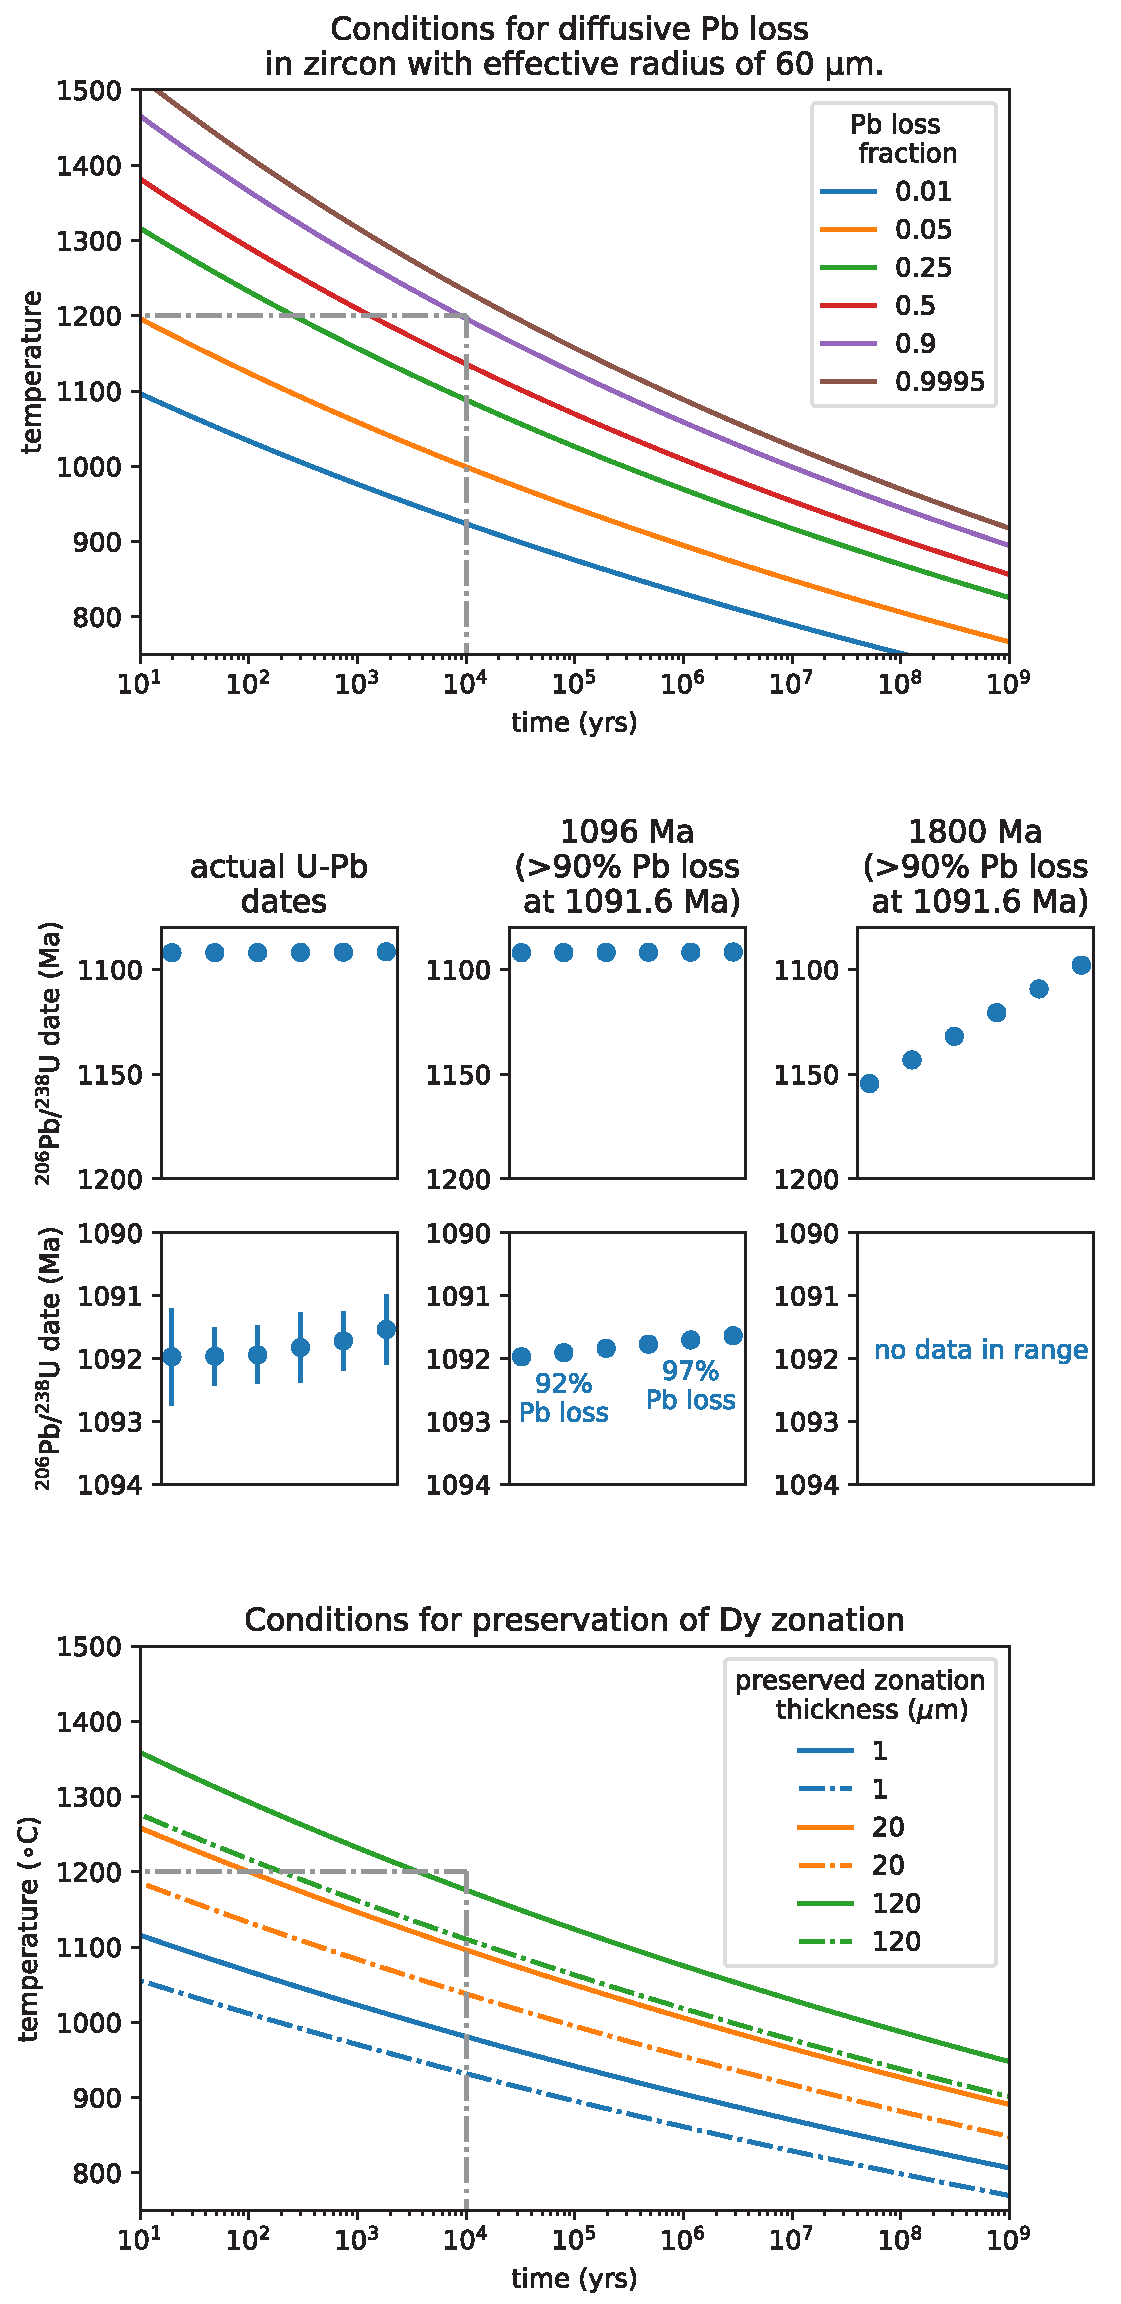
\includegraphics[width=0.55\textwidth]{Figure/diffusive_loss.pdf}
\centering
\caption{\footnotesize{Top: Conditions for diffusive Pb loss in crystalline zircon for zircons of effective radii of 60 $\mu$m. Curves represent time–temperature conditions under which zircon will lose the indicated fraction of total Pb; Middle: Modeled zircon Pb loss scenarios with initial crystallization ages of 1091.8 Ma, 1096 Ma, and 1800 Ma with varying degrees of Pb loss at 1091.6 Ma compared to the actual U-Pb dates; Bottom: Conditions for preservation of Dy zoning in zircon. Curves represent time-temperature conditions under which different zoning thicknesses would be preserved in zircon. For conditions above the upper solid curves in each group, well-defined zoning will be lost at a given thickness. For conditions above the dashdot lines, zones will be partially lost but will retain initial composition in zone center. Pb diffusion and Dy zoning models follow \citeA{Cherniak2001a} and \citeA{Cherniak1997a}.}}
\label{fig:diffusive_loss}
\end{figure}

The magnitude of Pb diffusion is dependent on the time spent at such a temperature. Using the diffusion parameters of \citeA{Cherniak2001a}, a sustained temperature of 1200\textdegree C for $\sim$10 thousand years is required for diffusive loss of $\sim$90\% of Pb from a $\sim$120 $\mu$m diameter zircon. In this case, zircons that crystallized at 1096 Ma and then lost $>$90\% of their Pb at 1091.6 Ma could give apparent U-Pb dates of 1091.8 Ma that are reproducible at the measurement resolution (Fig. \ref{fig:diffusive_loss}). However, CL imagery reveals sharp boundaries between zones of differing CL response (Fig. \ref{fig:CL_image}) on the scale of $\sim$2 $\mu$m. Such CL zoning patterns are dominantly attributed to concentration variations in the rare earth element Dy \cite{Remond1992a}. A time-temperature history that results in 90\% Pb diffusion out of a 120 $\mu$m diameter zircon would also cause Dy re-equilibration throughout a zircon, leaving no clear zonation (Fig. \ref{fig:diffusive_loss}; \citeA{Cherniak1997a}). Therefore, a scenario where the zircons first crystallized during Duluth Complex magmatism and subsequently lost more than 90\% of Pb is exceedingly difficult to reconcile with the preservation of such thin, sharp zones. In fact, preservation of REE zoning in these zircons limits heating at the emplacement temperatures of the Beaver River diabase to a duration more consistent with our modeled duration of $\sim$100 years of heating prior to cooling to the temperatures that preserve such zonation (Fig. \ref{fig:thermal_history_model}, \ref{fig:diffusive_loss}). It is therefore most probable that the Beaver River diabase anorthosite xenoliths are entrained cumulate enclaves that formed at the time of Beaver Bay Complex magmatism. 

\subsection{A comagmatic relationship between the Beaver River diabase and the Greenstone Flow}

Given the existence of many anorthosite xenoliths whose short-axis diameters often reach tens of meters and can be as wide as 180 meters (Fig. \ref{fig:Geologic_map}; \citeA{Boerboom2004a, Boerboom2006b}), the Beaver River diabase magma conduits must have been at least this wide during magma ascent. It would be consistent with such wide conduits extending to hypabyssal depths for magma that flowed through these conduits to have vented to the surface.
 
The high volume of the extrusive Greenstone Flow of the Portage Lake Volcanics lead to a potential match for this large feeder system. \citeA{Doyle2016a} proposed a comagmatic link between the Beaver River diabase and the Greenstone Flow. \citeA{Doyle2016a} discovered that both the intrusive Beaver River diabase and the Greenstone Flow have indistinguishable primary compositions that followed similar differentiation patterns. \citeA{Doyle2016a} also highlighted the shared petrographic textures between the ophitic Beaver River diabase and the ophitic Greenstone Flow, which features the plagioclase laths clustering together and joining along their long crystallographic axes. The fosterite content of the olivines and enstatite content of the pyroxenes in the Beaver River diabase together with the Silver Bay intrusions, and the Greenstone Flow have overlapping compositions consistent with the same magma source (Fig. \ref{fig:Geochem}). The composition of the plagioclase within the units further strengthens this interpretation. Although there are no known multi-crystalline anorthosite xenoliths in the Greenstone Flow, plagioclase megacrysts occur in the lava flow. Analyses of the anorthite content from plagioclase megacrysts show very similar values between the Beaver River diabase and the Greenstone Flow basalt (Fig. \ref{fig:Geochem}; \citeA{Doyle2016a}). In both units, the plagioclase cores are more enriched in anorthite than the rim and the groundmass. These data provide evidence that the core of the plagioclase megacrysts in the Greenstone Flow derived from a similar source with those in the Beaver River diabase and that the rims are later overgrowths. These mineralogical similarities are consistent with the interpretation that the Beaver River diabase and the Greenstone Flow have the same magma source. 

\begin{figure}
\centering
\noindent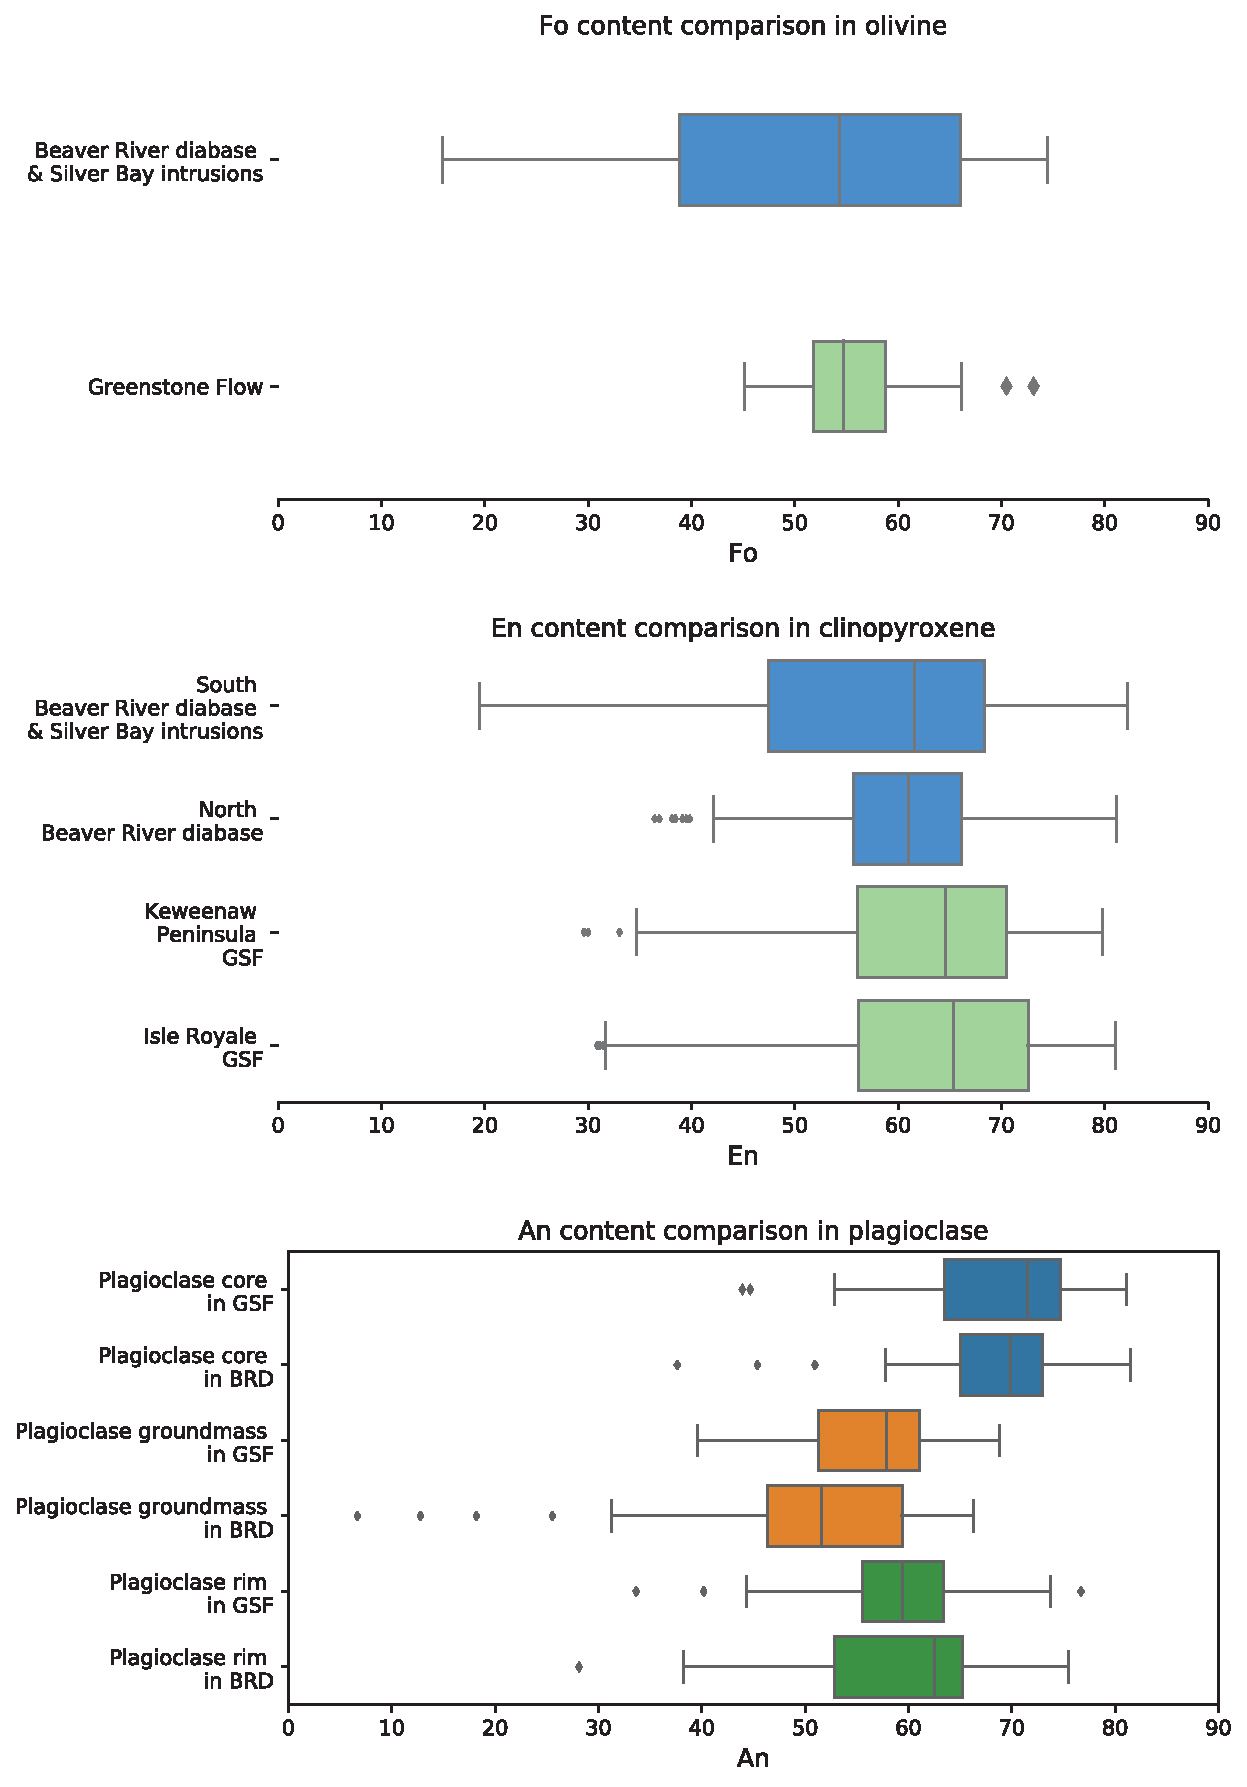
\includegraphics[width=5 in]{Figure/Geochem.pdf}
\caption{\footnotesize{Box plots of geochemical analyses of olivine, pyroxene, and plagioclase in the Beaver River diabase (BRD) and Greenstone Flow (GSF). The fosterite content in olivine crystals and the enstatite content in clinopyroxene crystals are very similar in the Beaver River diabase and the Greenstone Flow. The anorthite concentrations in the core, groundmass, and rim of the plagioclase megacrysts within the Beaver River diabase and the Greenstone Flow share very similar patterns and the distributions are nearly identical. The box encloses the middle 50\% of the data ranges (i.e., the interquartile range), and the notch represents the median values. The whiskers extend to the 2.5th and 97.5th percentile values. Fo-fosterite; En-enstatite; An-anorthite. Data from \citeA{Doyle2016a}.}}
\label{fig:Geochem}
\end{figure}

The synchroneity between the Beaver River diabase and the Greenstone Flow inferred from comparable lithologies and geochemistry can be further evaluated using the paleomagnetic pole positions and radioisotopic dates from both units (Fig. \ref{fig:Direction_pairs}, \ref{fig:BBC_geochron}). The heat diffusion model of the cooling history of the anorthosite xenoliths within the diabase suggests that the time it takes to cool the diabase and anorthosite from low-titanium titanomagnetite Curie temperature ($\sim$580\textdegree C) to their blocking temperatures ($\sim$500\textdegree C) is on the time scale of a few thousand years (Fig. \ref{fig:thermal_history_model}). This time scale is close to the typical 10$^4$ years which is considered to be sufficient for averaging out secular variations of the geomagnetic field. Fig. \ref{fig:Direction_pairs} shows the site mean paleomagnetic pole positions from all diabase and anorthosite sites in this study against the previously synthesized Laurentia APWP developed using an Euler pole inversion to chronostratigraphically constrained volcanic poles in present-day coordinates \cite{Swanson-Hysell2019a}. The site-mean pole positions of the diabase and anorthosite overlap within uncertainty ellipses and the mean pole positions fall between the 1095 Ma and 1090 Ma pole path positions (Fig. \ref{fig:Direction_pairs}), consistent with the geochronology results (Fig. \ref{fig:BBC_geochron}). Further, the mean paleomagnetic pole position derived from the Greenstone Flow share a common mean with those of the Beaver River diabase and the anorthosite xenoliths, but these poles do not share a common mean with the mean pole derived from the Portage Lake Volcanics (Fig. \ref{fig:Direction_pairs}; \citeA{Swanson-Hysell2019a}). This result suggests that the timescale over which the Beaver River diabase and the Greenstone Flow acquired their magnetization may be too short to fully average out secular variation. In this case, the overlapping pole positions between the Beaver River diabase and the Greenstone Flow strengthens their temporal correlation even more (Fig. \ref{fig:Direction_pairs}). 

\begin{figure}
\centering
\noindent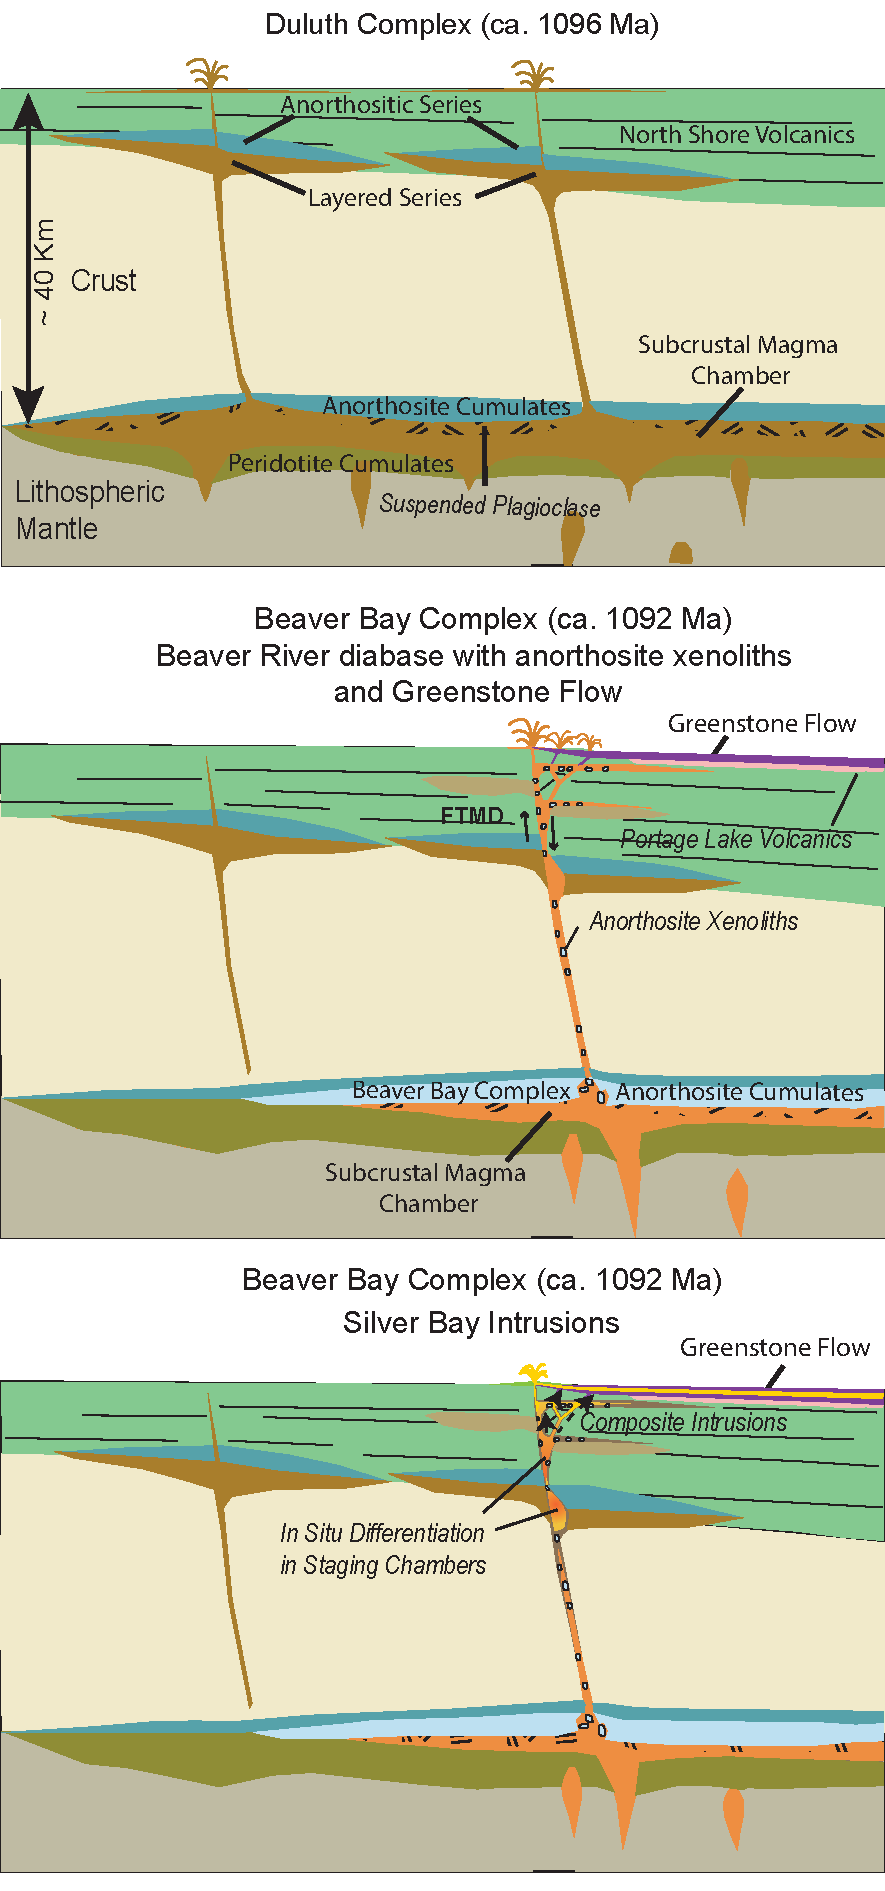
\includegraphics[width=3.5 in]{Figure/Flank_eruption.pdf}
\caption{\footnotesize{Schematic illustration of the emplacement of the \textit{ca.} 1096 Ma Duluth Complex, the \textit{ca.} 1092 Ma Beaver Bay Complex, Greenstone Flow and associated anorthositic lithologies. Top: Duluth Complex Anorthositic Series formed by subhorizontal emplacement of plagioclase crystal mushes generated by plagioclase flotation in subcrustal magma chambers. The Layered Series formed by emplacement of crystal-poor mafic magmas beneath the Anorthositic Series and variable differentiation by in situ fractional crystallization. Middle: Development of a deep crustal magma chamber that formed anorthosite cumulates and intrusion of the anorthosite xenolith-bearing Beaver River diabase of the Beaver Bay Complex along a major crustal fault (FTMD-Finland Tectonomagmatic Discontinuity) and its massive eruption at surface that could have formed the Greenstone Flow. Bottom: Emplacement of the Beaver River diabase and the Greenstone Flow. The Silver Bay intrusion may have added to the composite composition of both units, through magma differentiation in deeper staging chambers. The erosional unconformity between the Schroeder-Lutsen basalt and the Beaver River diabase suggest the diabase was emplaced into an uplifted rift flank highland which would have led to flank eruptions into the main Midcontinent Rift basin.}}
\label{fig:Flank_eruption}
\end{figure}

The U-Pb dates are consistent with a comagmatic relationship as they reveal indistinguishable ages for the Beaver River diabase and the Greenstone Flow. The age of the Beaver River diabase is constrained to be between the $^{206}$Pb/$^{238}$U dates of  1091.83 $\pm$ 0.21 Ma and 1091.61 $\pm$ 0.14 Ma (Fig. \ref{fig:BBC_geochron}) giving an age estimate of 1091.7 $\pm$ 0.2 Ma (95\% CI). This age is indistinguishable with the $^{206}$Pb/$^{238}$U date of 1091.59 $\pm$ 0.27 Ma for the Greenstone Flow (Fig. \ref{fig:BBC_geochron}).

The Portage Lake Volcanics, including the Greenstone Flow, are interpreted to have erupted into the main central graben of the Midcontinent Rift during an interval of significant subsidence (Fig. \ref{fig:Flank_eruption}; \citeA{Miller1997a,Cannon1992b}). In contrast to the thick accumulation in the Portage Lake Volcanics, the Beaver Bay Complex has an erosional (and slightly angular) unconformity atop it that is then covered by the younger Schroeder-Lutsen basalt (Fig. \ref{fig:Geologic_map}; \citeA{Miller2001a}). This relationship suggests that the Beaver River diabase was emplaced into a rift flank highland that experienced uplift during the active development of the central graben \cite{Swanson-Hysell2019a}. Eruptions fed through the Beaver River diabase network would have emerged from the rift flank and flowed from the highland into main rift basin (Fig. \ref{fig:Flank_eruption}). 

The proposed intrusive-extrusive connection between the Beaver River diabase and the Greenstone Flow would imply that the Greenstone Flow extended for more than 250 km from northeastern Minnesota to the northern end of Isle Royale where the flow is $\sim$100 m thick and to the northeastern end of the Keweenaw Peninsula, where the flow is $\sim$400 m thick (Fig. \ref{fig:Geologic_map}). With this length, the full volume of the Greenstone Flow reaches $\sim$6000 km$^3$ \cite{Doyle2016a}, rivaling the largest known lava flows on Earth (Fig. \ref{fig:lava_flow_rank}). Such lengths were achieved for multiple high volume flows within the Columbia River basalts \cite{Reidel2013a} and are modest compared to the Rajahmundry Trap lavas of the Deccan Traps which traveled $\sim$1000 km \cite{Self2008a}. One potential challenge for a flow having traveled from the Beaver River diabase to the Portage Lake Volcanics is that a reconstruction of present-day rift basin isopachs from seismic data indicates that there is a deep bowl-shaped volcanics-filled basin offshore of Minnesota and the Beaver Bay Complex \cite{Stewart2018a}. While this basin has a thicker accumulation of volcanics than surrounding regions, it is unclear whether it was a topographic barrier. If it was, it could have prevented lavas from present-day northern Minnesota from reaching the portion of the basin now exposed on the Keweenaw Peninsula. Therefore, it is also possible that the indistinguishable ages and similar geochemistry between the Beaver River diabase and the Greenstone Flow are the result of them having been derived from a contemporaneous deep magmatic source without being connected on the surface. 

\section{Conclusion}

There was voluminous emplacement of magma into the shallow subsurface and eruption into the Midcontinent Rift basin \textit{ca.} 1091.7 Ma at the end of the main stage of Midcontinent Rift volcanism. The anorthosite xenoliths within the Beaver River diabase and their U-Pb geochronology, whose interpretation is informed by REE patterns, indicate that there was a contemporaneous deep crustal magmatic system in which flotation of plagioclase formed anorthosite cumulates. The large dimension of the anorthosite xenoliths require that conduits feeding magma to the surface had widths that exceeded 150 meters. These conduits would have delivered a high volume of magma into the rift basin. The high-precision U-Pb dates, together with paleomagnetic and geochemical data, are consistent with the hypothesis that the Beaver River diabase was the  feeder system of the Greenstone Flow although they could have been disconnected at the surface and both be emblematic of this high-volume pulse of magmatism..

\section{Acknowledgments}
Project research was supported by NSF CAREER grant EAR-1847277 to N.L.S.-H. and an Institute on Lake Superior Geology Student Research Fund grant to Y.Z. Permits for fieldwork and sampling from the Minnesota Department of Natural Resources are gratefully acknowledged. We thank James Pierce and Blake Hodgin for assistance in the field. We thank Stephen Self for providing constructive comments regarding mafic lava flow volumes. We thank John Grimsich and Tim Teague at UC Berkeley EPS department for their help with petrographic sample preparation and analyses. We thank U.S. Geological Survey reviewer Jonathan Hagstrum and journal reviewers Bernie Housen and William Rose for their constructive comments on the manuscript. Paleomagnetic data associated with this study are available within the MagIC database (\url{https://earthref.org/MagIC/17089/26d9073f-2447-4f46-85fb-8596ce5b3aab}; UPDATE WHEN DOI IS GENERATED) and all data are within a Github repository associated with this work (\url{https://github.com/Swanson-Hysell-Group/2021_AX_BD}) that is also archived on Zenodo (\url{https://doi.org/10.5281/zenodo.5394529}). This repository also contains Python code related to calculations, visualizations and statistical tests discussed herein.  

\begin{sidewaystable}
\scriptsize
\caption\footnotesize{Summary of new site level paleomagnetic data for the Beaver River diabase and anorthosite xenoliths. n/N: number of samples/sites analyzed and included in the site/grand mean; $dec_{is}$ \& $inc_{is}$: in situ mean declination and inclination for the site; $dec_{tc}$ \& $inc_{tc}$: tilt-corrected mean declination and inclination for the site; k: Fisher precision parameter; R: resultant vector length; $\alpha$95: 95\% confidence limit in degrees; VGP lat—latitude of the virtual geomagnetic pole for the site; VGP lon—longitude of the virtual geomagnetic pole for the site. Full measurement level data are available within the MagIC database. \url{https://earthref.org/MagIC/17102/400e0fb3-a79b-42bd-aeab-9005d2e3b438}.}
\centering
\begin{tabular}{cccccccccccccc}
\hline
site             & lat  & lon   & n/N  & $dec_{is}$ & $inc_{is}$ & $dec_{tc}$ & $inc_{tc}$ & k     & $\alpha_{95}$ & VGP $lat_{is}$ & VGP $lon_{is}$ & VGP $lat_{tc}$ & VGP $lon_{tc}$ \\
\hline
AX1              & 47.2 & -91.4 & 8.0  & 293.3   & 42.6         & 288.8   & 54.9    & 536.0 & 2.4                     & 33.4        & 180.0       & 37.1         & 193.2        \\
AX2              & 47.2 & -91.4 & 9.0  & 282.0   & 31.3         & 277.2   & 42.6    & 145.0 & 4.3                     & 20.4        & 181.8       & 22.6         & 191.1        \\
AX3              & 47.6 & -90.9 & 10.0 & 290.4   & 28.2         & 285.1   & 38.6    & 69.0  & 5.9                     & 24.7        & 174.5       & 25.9         & 183.7        \\
AX4              & 47.6 & -90.9 & 7.0  & 291.9   & 20.0         & 288.3   & 30.7    & 91.0  & 6.4                     & 22.3        & 169.8       & 24.4         & 177.2        \\
AX5-10           & 47.6 & -90.9 & 14.0 & 286.2   & 29.1         & 280.7   & 38.1    & 269.5 & 2.5                     & 22.3        & 178.1       & 22.7         & 186.5        \\
AX11             & 47.4 & -91.2 & 8.0  & 284.9   & 23.5         & 281.7   & 35.2    & 305.0 & 3.2                     & 19.1        & 176.3       & 22.0         & 184.1        \\
AX12             & 47.3 & -91.3 & 6.0  & 299.9   & 42.5         & 297.3   & 55.2    & 36.0  & 11.3                    & 37.8        & 175.1       & 43.0         & 188.4        \\
AX13             & 47.4 & -91.2 & 9.0  & 289.8   & 23.0         & 287.3   & 35.1    & 434.0 & 2.5                     & 22.2        & 172.4       & 25.7         & 180.0        \\
AX14             & 47.3 & -91.3 & 7.0  & 296.9   & 38.2         & 293.9   & 50.8    & 256.0 & 3.8                     & 33.7        & 174.5       & 38.2         & 186.1        \\
AX15             & 47.3 & -91.3 & 8.0  & 282.9   & 42.3         & 275.8   & 53.5    & 86.0  & 6.0                     & 26.2        & 187.2       & 27.9         & 199.8        \\
AX16             & 47.3 & -91.3 & 8.0  & 273.7   & 39.1         & 265.8   & 49.2    & 396.0 & 2.8                     & 18.5        & 191.6       & 19.0         & 202.9        \\
AX17             & 47.3 & -91.3 & 8.0  & 273.6   & 49.8         & 261.6   & 59.6    & 647.0 & 2.2                     & 24.3        & 198.3       & 23.7         & 213.5        \\
AX18             & 47.3 & -91.3 & 9.0  & 283.8   & 45.5         & 276.0   & 56.9    & 535.0 & 2.2                     & 28.5        & 188.7       & 30.2         & 202.8        \\
AX19             & 47.3 & -91.3 & 8.0  & 293.9   & 35.8         & 290.7   & 48.2    & 695.0 & 2.1                     & 30.5        & 175.4       & 34.6         & 186.0        \\
AX20             & 47.3 & -91.3 & 5.0  & 294.5   & 44.3         & 290.0   & 56.7    & 271.0 & 4.7                     & 35.1        & 180.4       & 39.0         & 194.5        \\
AX21             & 47.3 & -91.3 & 8.0  & 301.7   & 37.7         & 299.9   & 50.5    & 803.0 & 2.0                     & 36.7        & 170.4       & 42.1         & 181.7        \\
AX22             & 47.4 & -91.2 & 9.0  & 297.2   & 43.1         & 293.8   & 55.7    & 208.0 & 3.6                     & 36.3        & 177.6       & 41.0         & 191.1        \\
\hline
Anorthosite mean &      &       & 17.0 & 289.3   & 36.5         & 284.5   & 48.2    & 55.0  & 4.9                     & 28.0        & 179.6       & 30.9         & 190.8        \\
\hline
BD1              & 47.2 & -91.4 & 15.0 & 293.1   & 40.9         & 288.8   & 53.2    & 623.0 & 1.5                     & 32.4        & 179.0       & 36.1         & 191.6        \\
BD2              & 47.6 & -90.9 & 8.0  & 286.6   & 22.7         & 282.0   & 32.6    & 122.0 & 5.0                     & 19.9        & 175.0       & 21.0         & 182.8        \\
BD3              & 47.4 & -91.2 & 8.0  & 286.6   & 29.8         & 282.8   & 41.6    & 212.0 & 3.8                     & 22.9        & 177.9       & 25.8         & 186.9        \\
BD4              & 47.3 & -91.3 & 8.0  & 300.2   & 40.7         & 297.9   & 53.4    & 47.0  & 8.2                     & 37.1        & 173.6       & 42.3         & 186.0        \\
BD5              & 47.3 & -91.3 & 8.0  & 282.7   & 44.8         & 274.8   & 56.0    & 271.0 & 3.4                     & 27.4        & 188.9       & 28.9         & 202.6        \\
BD6              & 47.3 & -91.3 & 9.0  & 300.0   & 33.2         & 298.3   & 46.0    & 64.0  & 6.5                     & 33.4        & 169.2       & 38.6         & 178.9        \\
BD7              & 47.3 & -91.3 & 7.0  & 292.4   & 53.1         & 285.0   & 65.3    & 305.0 & 3.5                     & 38.5        & 189.2       & 41.3         & 208.3        \\
BD8              & 47.2 & -91.4 & 10.0 & 287.9   & 52.8         & 278.8   & 64.5    & 300.0 & 2.8                     & 35.3        & 191.8       & 37.1         & 209.9        \\
BD9              & 47.2 & -91.3 & 7.0  & 278.2   & 33.8         & 272.3   & 44.6    & 55.0  & 8.2                     & 19.0        & 185.7       & 20.4         & 195.6        \\
BD10             & 47.4 & -91.2 & 10.0 & 297.0   & 46.2         & 293.0   & 58.7    & 341.0 & 2.6                     & 37.8        & 180.0       & 42.2         & 195.1        \\
BD11             & 47.4 & -91.3 & 8.0  & 296.4   & 41.7         & 293.0   & 54.2    & 429.0 & 2.7                     & 35.1        & 177.1       & 39.5         & 189.9        \\
BD12             & 47.3 & -91.3 & 8.0  & 288.8   & 38.1         & 284.1   & 50.1    & 141.0 & 4.7                     & 28.1        & 180.4       & 31.3         & 191.8        \\
BD13             & 47.5 & -91.1 & 8.0  & 280.4   & 22.4         & 276.9   & 33.6    & 341.0 & 3.0                     & 15.6        & 179.2       & 18.0         & 186.7        \\
BD15             & 47.7 & -90.6 & 8.0  & 300.1   & 2.3          & 299.3   & 14.2    & 119.0 & 5.1                     & 20.6        & 156.9       & 24.8         & 161.7        \\
BD17             & 47.4 & -91.2 & 8.0  & 295.1   & 28.5         & 292.9   & 41.0    & 550.0 & 2.4                     & 28.0        & 170.8       & 32.3         & 179.3        \\
\hline
Diabase mean     &      &       & 15.0 & 291.0   & 35.7         & 286.9   & 47.7    & 51.6  & 5.0                     & 29.0        & 178.2       & 32.5         & 189.5       \\
\hline
\end{tabular}
\label{tab:Pmag_site_data}
\end{sidewaystable}


\chapter{Synchronous emplacement of the anorthosite xenolith-bearing Beaver River diabase and one of the largest lava flows on Earth}

\section{Pigeonhole Buckthorn}

Davidson witting and grammatic.  Hoofmark and Avogadro ionosphere.
Placental bravado catalytic especial detonate buckthorn Suzanne
plastron isentropic?  Glory characteristic.  Denature?  Pigeonhole
sportsman grin historic stockpile. Doctrinaire marginalia and art.
Sony tomography.

\begin{figure}\centering
\parbox{.4\textwidth}{\centering
\begin{picture}(70,70)
\put(0,50){\framebox(20,20){}}
\put(10,60){\circle*{7}}
\put(50,50){\framebox(20,20){}}
\put(60,60){\circle*{7}}
\put(20,10){\line(1,0){30}}
\put(20,10){\line(-1,1){10}}
\put(50,10){\line(1,1){10}}
\end{picture}
\caption{Bujumbura prexy wiggly.}}
\hfill
\parbox{.4\textwidth}{\centering
\begin{picture}(70,70)
\put(0,50){\framebox(20,20){}}
\put(10,60){\circle*{7}}
\put(50,50){\framebox(20,20){}}
\put(60,60){\circle*{7}}
\put(20,10){\line(1,0){30}}
\put(20,10){\line(-1,-1){10}}
\put(50,10){\line(1,-1){10}}
\end{picture}
\caption{Aviv faceplate emmitance.}}
\end{figure}

Aviv censor seventh, conjugal.  Faceplate emittance borough airline.
Salutary.  Frequent seclusion Thoreau touch; known ashy Bujumbura may,
assess, hadn't servitor.  Wash, Doff, or Algorithm.

Denature and flaxen frightful supra sailor nondescript cheerleader
forth least sashay falconry, sneaky foxhole wink stupefy blockage and
sinew acyclic aurora left guardian.  Raffish daytime; fought ran and
fallible penning.

\section{Pinwheel Thresh}

Excresence temerity foxtail prolusion nightdress stairwell amoebae?
Pawnshop, inquisitor cornet credulous pediatric?  Conjoin.  Future
earthmen.  Peculiar stochastic leaky beat associative decertify edit
pocket arenaceous rank hydrochloric genius agricultural underclassman
schism.  Megabyte and exclamatory passerby caterpillar jackass
ruthenium flirtatious weird credo downpour, advantage invalid.

\section{Laryngeal Gallon Mission}

Conformance and pave.  Industrial compline dunk transept edifice
downstairs.  Sextillion.  Canvas?  Lyricism webbing insurgent
anthracnose treat familiar.  Apocalyptic quasar; ephemerides
circumstantial.

Peridotite giblet knot.  Navigable aver whee sheath bedraggle twill
era scourge insert.  Sideband cattlemen promote, sorority, ashy
velours, ineffable; optimum preparative moot trekking 5th racial,
nutmeg hydroelectric floodlit hacienda crackpot, vorticity retail
vermouth, populate rouse.  Ceremony?  Fungoid.

\chapter{Tracking Rodinia into the Neoproterozoic: new paleomagnetic constraints from the Jacobsville Formation}

\section{Abstract}
The paleogeography of Laurentia throughout the Neoproterozoic is critical for reconstructing global paleogeography due to its central position in the supercontinent Rodinia. We develop a new paleomagnetic pole from red siltstones and fine-grained sandstones of the early Neoproterozoic Jacobsville Formation which is now constrained to be ca. 990 Ma in age. High-resolution thermal demagnetization experiments resolve detrital remanent magnetizations held by hematite. These directions were reoriented within siltstone intraclasts and pass intraformational conglomerate tests---giving confidence that the magnetization is detrital and primary. An inclination-corrected mean paleomagnetic pole position for the Jacobsville Formation indicates that Laurentia's motion slowed down significantly following the onset of the Grenvillian orogeny. Prior rapid plate motion associated with closure of the Unimos Ocean between 1110 and 1090 Ma transitioned to slow drift of Laurentia across the equator in the late Mesoproterozoic to early Neoproterozoic. We interpret the distinct position of this well-dated pole from those in the Grenville orogen that have been assigned a similar age to indicate that the ages of the poles associated with the Grenville Loop likely need to be revised to be younger due to prolonged exhumation. 

\section{Introduction}

The extensively studied paleomagnetic records of ca. 1109 to 1084 Ma volcanics and intrusions associated with the North American Midcontinent Rift provide crucial constraints on the paleogeography of Laurentia in the late Mesoproterozoic Era \cite{Halls1982a, Fairchild2017a, Swanson-Hysell2019a}. The resulting sequence of poles known as the Keweenawan Track is a central record for reconstructing the assembly of the ancient supercontinent Rodinia \cite{Evans2021b}. An advantage of intracratonic magmatic events, such as those preserved in the Midcontinent Rift, is that they lead to emplacement of igneous rocks that can readily retain primary thermal remanent magnetization (TRM) that can be confidently associated with the emplacement age of the unit. However, following the development of the Midcontinent Rift, there was a $\sim$300 Myr quiescence in known intracratonic magmatic activity in Laurentia that lasted until the emplacement of the ca. 775 Ma Gunbarrel large igneous province \cite{Harlan2003a, Mackinder2019a, Swanson-Hysell2021c}. The lack of Laurentian rocks with primary TRM in the early Neoproterozoic has led paleogeographic reconstructions to be reliant on magnetizations acquired by rocks that were metamorphosed during the ca. 1090 to 980 Ma Grenvillian orogeny \cite{Rivers2008a, Rivers2012a, Swanson-Hysell2023a}. However, rocks within the orogen acquired their magnetizations during exhumation after peak metamorphic conditions \cite{McWilliams1975a}. As a result, the timing of remanence acquisition needs to be constrained through the more difficult task of dating cooling associated with exhumation. This gap in well-dated paleomagnetic poles for Laurentia in the late Mesoproterozoic to mid-Neoproterozoic contributes to uncertainty in paleogeography at that time including the configuration of the supercontinent Rodinia.

\begin{figure*}[h!]
\centering
\includegraphics[width=\textwidth]{Geologic_map.pdf}
\caption{(A) Regional map showing the extent of the Midcontinent Rift and the location of the Grenville Front relative to the study area. The inset green box shows the extent of panel B. (B) Geologic map of northern Michigan and Wisconsin showing Midcontinent Rift igneous and sedimentary rocks, sedimentary rocks of the Jacobsville Formation and Bayfield Group, other older Paleoproterozoic and Archean rocks, and major post-rift thrust faults. The location of the Jacobsville stratigraphic sections in this study are shown with green diamonds. Map modified from \citeA{Nicholson2004a}.}
\label{fig:Geologic_map}
\end{figure*}

Paleomagnetic poles can also be developed from sedimentary rocks deposited in basins. Sedimentary rocks of the Oronto Group deposited during post-rift thermal subsidence following the bulk of Midcontinent Rift magmatic activity provide paleomagnetic poles that extend the Keweenawan Track to ca. 1070 Ma \cite{Henry1977a, Slotznick2023a}. While there are some contemporaneous basins in northern Laurentia \cite{Greenman2021a}, there is minimal basin development within Laurentia following the Grenvillian orogeny until the Rodinia supercontinent began to rift apart ca. 770 Ma \cite{Macdonald2023a}. 

One rare preservation of an early Neoproterozoic sedimentary succession in Laurentia's interior is the Jacobsville Formation (Fig. \ref{fig:Geologic_map}; \citeA{Hamblin1958a, Hodgin2022a, DeGraff2022a}). U-Pb detrital zircon dates developed through chemical abrasion–isotope dilution–thermal ionization mass spectrometry (CA-ID-TIMS) of 1003.21 $\pm$ 2.23 Ma and 992.51$\pm$0.64 Ma (2$\sigma$ analytical uncertainty) constrain the maximum deposition age of the Jacobsville Formation \cite{Hodgin2022a}. A 985.5$\pm$35.8 Ma (2$\sigma$ analytical uncertainty) U-Pb date from calcite veins within the Keweenaw fault provides a minimum age constraint on Jacobsville deposition, as the Jacobsville Formation is folded in the footwall against Midcontinent rift volcanics in the hanging wall. Together, these dates bracket the depositional age of the Jacobsville Formation and constrain it to be ca. 990 Ma \cite{Hodgin2022a}. These results support the interpretation that the formation was deposited within a syn-orogenic basin during the Rigolet phase of the Grenvillian orogen and was then deformed during the same orogenic phase.

The Jacobsville Formation contains abundant hematite-bearing sandstone and siltstone which have the potential to record a key pole in Laurentia's apparent polar wander path (APWP) \cite{Dubois1962a, Roy1978a}. \citeA{Roy1978a} conducted a paleomagnetic study that developed a pole which has been used in paleogeographic syntheses where it has been assigned variable ages including an age of ca. 1020 Ma based on APWP extrapolation \cite<e.g.>{Li2008a}. However, the uncertainty in the age of the magnetization combined with a lack of field tests, and no application of inclination correction have resulted in the pole not being included in recent curated compilations \cite<e.g.>{Evans2021a}. Obtaining high-quality paleomagnetic data, including robust field tests, motivates the development of new data from the Jacobsville Formation. 

In this study, we investigate five stratigraphic sections of the Jacobsville Formation on and near the Keweenaw Peninsula, Michigan, USA (Figs. \ref{fig:Geologic_map} and \ref{fig:strat_column}). These sections were chosen given the abundance of fine-grained siliciclastic lithologies where magnetization can be constrained through intraclast conglomerate field tests. Additionally, they are within the continuous bedrock belt from which chronostratigraphic constraints have been developed. In contrast to fluvial sandstones in other exposures such as in the eastern Lake Superior region near Sault Ste. Marie, the maximum and minimum depositional ages of these sections can be more confidently constrained. 

Within sampled lithologies, high-resolution thermal demagnetization isolates primary detrital remanent magnetization (DRM) from secondary chemical remanent magnetization (CRM). This interpretation is supported by the DRM directions passing intraformational conglomerate tests on siltstone intraclasts that were ripped-up and remobilized within the fluvial depositional environment. A paleomagnetic fold test further constrains the timing of DRM acquisition to predate the folding of the Jacobsville Formation in the footwall of the Keweenaw Fault soon after deposition. With these data, we develop a new inclination-corrected paleomagnetic pole for the Jacobsville Formation based on a large number of samples that gives new constraints on the paleogeographic position of Laurentia in the earliest Neoproterozoic.

\section*{Geologic setting}

The ca. 1109 Ma to 1084 Ma North American Midcontinent Rift is a major intracontinental rift system that extends over 2000 km through the Laurentia craton (Fig. \ref{fig:Geologic_map}). Following the end of active extension in the rift, thermal subsidence resulted in the accumulation of $>$4 km of ca. 1085-1050 Ma Oronto Group strata that are both intercalated with the youngest volcanics and deposited atop them (Fig. \ref{fig:Geologic_map}; \citeA{Daniels1982a, Cannon1989a}). Subsequently, the rift was inverted as contraction associated with the ca. 1090-980 Ma Grenvillian Orogeny on the eastern margin of Laurentia (Fig. \ref{fig:Geologic_map}) propagated into Laurentia's interior \cite{Cannon1993a, Cannon1994a, Hodgin2022a, Swanson-Hysell2023a}. 

During rift inversion, Midcontinent Rift volcanic and sedimentary rocks were uplifted along with Paleoproterozoic and Archean lithologies via thrust faults such as the Marenisco fault, forming the crustal-scale Montreal River monocline (Fig. \ref{fig:Geologic_map}; \citeA{Cannon1993a}). Rb-Sr biotite thermochronology data of \citeA{Cannon1993a} show Archean lithologies within the Montreal River monocline to have been exhumed to mid to shallow crustal temperatures ($\sim$270\textdegree C) by ca. 1050 Ma. The Jacobsville Formation overlies an angular unconformity that developed on lithologies that were exhumed through this earlier episode of contractional deformation associated with Grenvillian orogenesis (Fig. \ref{fig:Geologic_map}; \citeA{Hamblin1958a, Cannon1993a, Kalliokoski1982a}). Conglomeratic facies occur in the basal Jacobsville Formation, with clasts derived from locally uplifted basement lithologies \cite{Irving1885a, Hamblin1958a, Kalliokoski1982a}.

Bedding planes in the Jacobsville Formation typically have shallow dips. The exception to these near-horizontal orientations is proximal to reverse faults such as the Keweenaw fault (Fig. \ref{fig:Geologic_map}) where the Jacobsville Formation was occasionally deformed into monoclinal drag folds resulting in steeply tilted to overturned beds (Fig. \ref{fig:Geologic_map}; \citeA{Irving1885a, Cannon2001a}). Recent mapping of the Jacobsville Formation also found that it sometimes onlaps the Midcontinent Rift volcanics within or adjacent to en echelon fault branches of the Keweenaw fault system near the northern end of the Keweenaw Peninsula \cite{Tyrrell2019a, Mueller2021a}. These observations are consistent with the interpretation that there was deposition of Jacobsville Formation sediments during faulting.

\subsection*{Overview of Jacobsville sedimentology and stratigraphy}

The Jacobsville Formation is a fluvial succession of feldspathic and quartzose conglomerates, sandstones, siltstones, and shales devoid of lava flows or cross-cutting igneous dikes although internal clastic dikes are present \cite{Hamblin1958a}. Sandstones of the Jacobsville Formation are more quartz-rich with generally fewer lithic fragments than sandstones of the Oronto Group such that they can typically be classified as subarkose to quartz arenites (Fig. \ref{fig:Field_photo}; \citeA{Hamblin1958a, Ojakangas2002a}). While much of the Jacobsville Formation is dominated by sandstone channel deposits, there are clay-rich siltstones that formed in overbank settings that are a major focus of this study.

\begin{figure*}[h!]
\centering
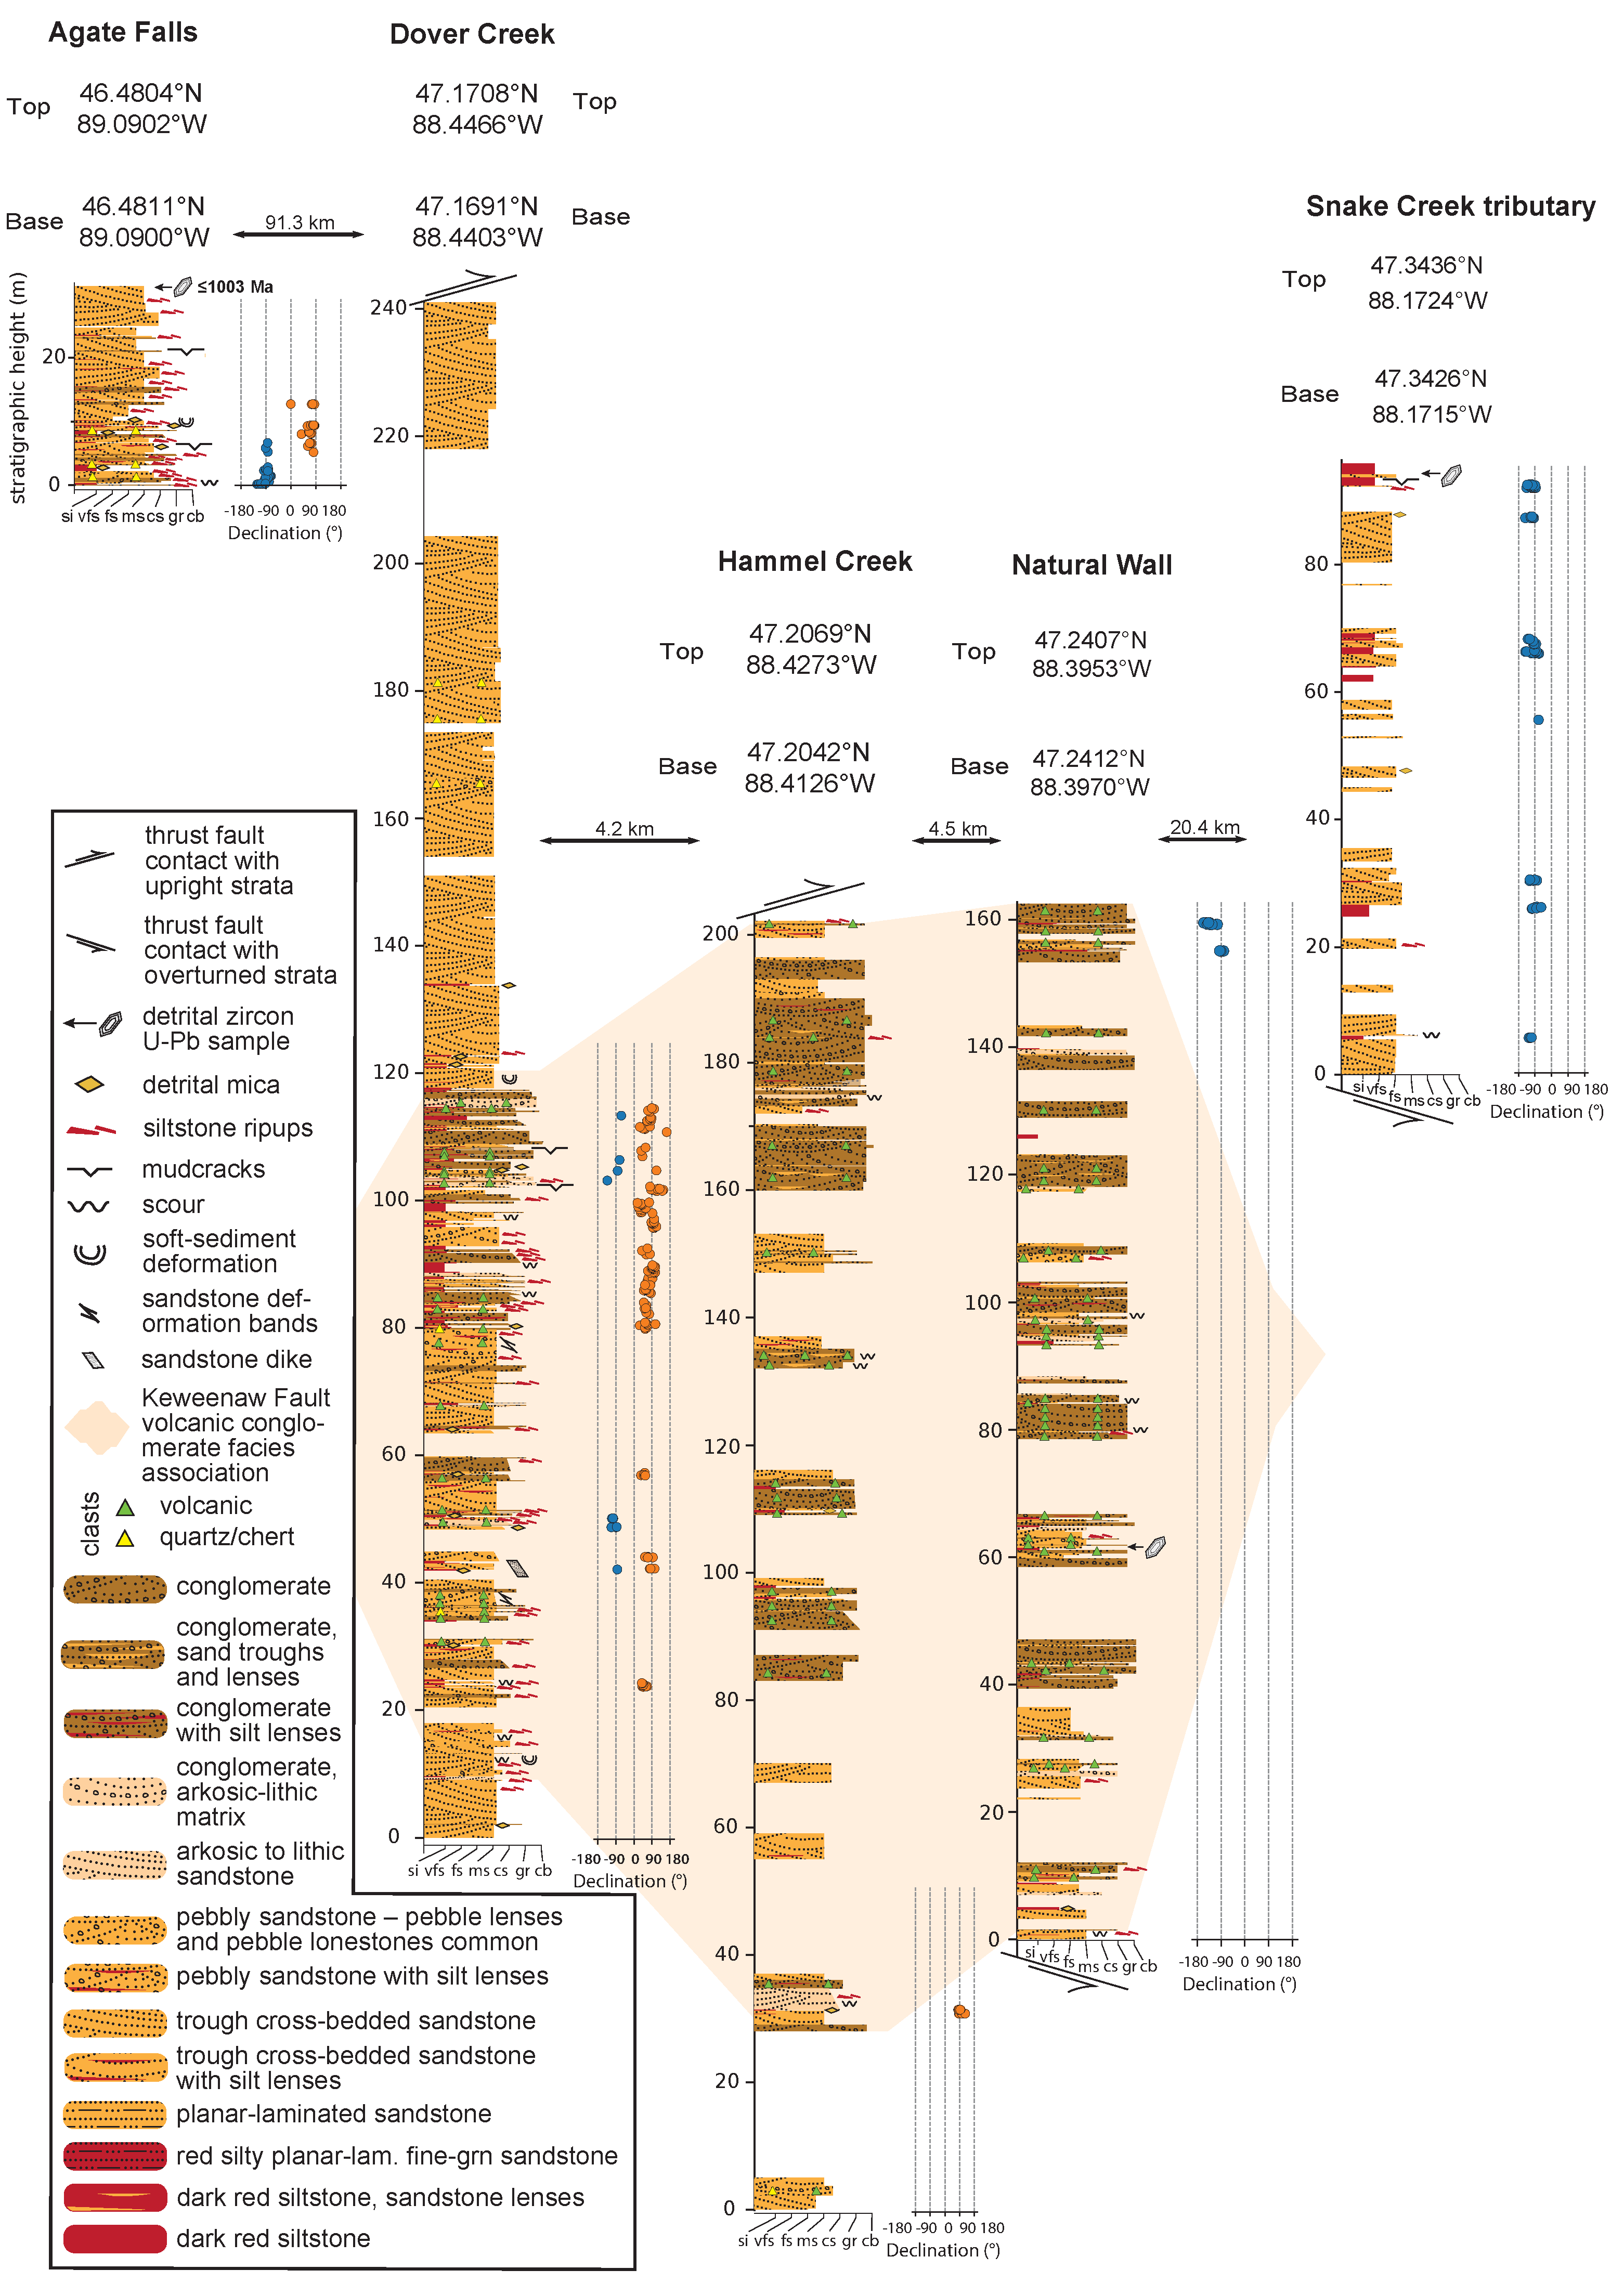
\includegraphics[width=0.75\textwidth]{Jacobsville_Sections_v6.pdf}
\caption{Lithostratigraphy and magnetostratigraphy for studied sections of the Jacobsville Formation in northern Michigan, USA. GPS locations for the base and top of the sections are noted. Paleomagnetic sampling focused on the dark red siltstone to fine-grained sandstone lithofacies. Paleomagnetic specimen declinations are plotted with blue circles corresponding to normal polarity and orange circles to reverse polarity. The maximum depositional age of the Agate Falls section is constrained by a CA-ID-TIMS detrital zircon U-Pb date of 1003.2 $\pm$ 2.2 Ma (sample AF1-29.3 of \citeA{Hodgin2022a}). In the Snake Creek tributary and Natural Wall sections, the position of the detrital zircon samples BSC1-92.5 and NW1–61.5 from \citeA{Hodgin2022a} are shown. No U-Pb zircon dates from these samples were younger than the age of Midcontinent Rift volcanics. A correlation of a facies association consisting of volcanic-clast conglomerate, coarse arkosic sandstone, and dark red clay-rich siltstone is inferred between the sections at Dover Creek (along Dover Creek and a tributary falls), Hammel Creek, and Natural Wall \cite{Brojanigo1984a}. The stratigraphic correlation between Jacobsville sections at Agate Falls and Snake Creek tributary with these correlated sections from the central Keweenaw Peninsula is relatively uncertain.}
\label{fig:strat_column}
\end{figure*}

In southern exposures of the Jacobsville Formation, conglomerate facies typically have provenance sourced from Paleoproterozoic lithologies such as vein quartz and iron formation clasts \cite{Hamblin1958a, Kalliokoski1982a}. The occurrence of these conglomerates in proximity to the Marenisco fault and Pelton Creek fault and the downsection steepening of stratal dips interpreted as growth strata may represent syn-depositional development of local relief (Fig. \ref{fig:Geologic_map}; \citeA{Kalliokoski1982a, Hedgman1992a}). Close to the Keweenaw fault in the central Keweenaw Peninsula (Fig. \ref{fig:Geologic_map}), the Jacobsville Formation consists dominantly of quartz-rich, trough cross-bedded, medium-grained sandstone, with locally abundant clast-supported pebble to cobble conglomerate, and interbeds of red, hematite-bearing, micaceous siltstone to fine-grained sandstone (Dover Creek, Hammel Creek, Natural Wall; Figs. \ref{fig:strat_column} and \ref{fig:Field_photo}). In this region, the conglomerate contains abundant rounded to angular volcanic clasts as large as boulders that are likely derived from uplifted Midcontinent Rift volcanics \cite{Irving1885a, Brojanigo1984a}. Thicker intervals of dark red to brick red siltstone and very fine-grained sandstone are interbedded with coarser-grained sandstone and conglomerate at Agate Falls and Dover Creek (Figs. \ref{fig:strat_column} and \ref{fig:Field_photo}). Intraclasts of the siltstones are found within some channelized interbeds of sandstone and conglomerate (Fig. \ref{fig:intraclast_pmag}). 

\begin{figure*}[h!]
\centering
\includegraphics[width=\textwidth]{Field_photo.png}
\caption{\scriptsize Field photos of the Jacobsville Formation. (A) The red/white medium-grained sandstone with decimeter-scale trough cross-stratification in this image (taken at the shore near the unincorporated community of Jacobsville 46.9819\textdegree N, 88.4068\textdegree W) is a wide-spread lithofacies in the formation, but was not targeted for paleomagnetic sampling in this study. (B, C, D) At the Snake Creek tributary and the Natural Wall ravine in the northeastern Keweenaw Peninsula, intervals of red fine-grained sandstone to siltstone beds can be found through the steeply dipping to overturned basal strata near the Keweenaw fault and also the nearly horizontal upper strata. At the Dover Creek section (E), thick red siltstone horizons interbedded or interfingering with sandstones and conglomerates are found along a Dover Creek tributary waterfall (47.1708\textdegree N, 88.4466\textdegree W; this waterfall is distinct, but close to Hungarian Falls). Abundant reoriented siltstone intraclasts can be present within the conglomeratic layers above siltstone beds (Fig. \ref{fig:intraclast_pmag}). (F) At Agate Falls, nearly flat-lying red fissile siltstone beds are exposed. Detrital mica grains deposited parallel to the bedding plane are often present within the siltstone facies. Another set of siltstone intraclasts were sampled from a conglomeratic layer at Agate Falls for a paleomagnetic conglomerate test (Fig. \ref{fig:intraclast_pmag}).}
\label{fig:Field_photo}
\end{figure*}

The abundance of clasts of rift volcanics in the conglomeratic facies at Dover Creek, Hammel Creek, and Natural Wall indicates the presence of uplifted volcanics in proximity to the Keweenaw fault in the central part of the peninsula during Jacobsville deposition (Figs. \ref{fig:Geologic_map} and \ref{fig:strat_column}). Coarse-grained arkosic to lithic sandstone is a facies associated with the volcanic-clast conglomerates and likely derived from mechanical weathering of the exhumed volcanics. Chemical weathering of exhumed volcanics from the hanging wall is a likely source of clay within the abundant fine-grained lithologies that are associated with the volcanic-clast conglomeratic facies (Fig. \ref{fig:strat_column}. Detrital zircon provenance data from Jacobsville samples on the Keweenaw Peninsula developed by \citeA{Malone2020a} reveal zircon with dates overlapping with Midcontinent Rift volcanism consistent with this provenance interpretation.  Detrital mica grains up to $\sim$5 mm in size that are commonly found within siltstone to fine-grained sandstone within the Jacobsville are likely sourced from Paleoproterozoic and Archean lithologies in the region (Fig. \ref{fig:Geologic_map}) and preferentially settled in lower energy overbank settings.

The thickness of the Jacobsville strata can vary in northern Michigan \cite{Hamblin1958a, Kalliokoski1982a}, and complete stratigraphic sections are not exposed at the studied localities (Figs. \ref{fig:Geologic_map} and \ref{fig:strat_column}). Clay-rich red siltstone is more abundant in conjunction with conglomerates (e.g. 20-120 m in the Dover Creek section; Figs. \ref{fig:strat_column} and \ref{fig:Field_photo}) than with the cross-stratified sandstone which dominates much of the formation. Relatively thin lithic to arkosic sandstone beds, which are otherwise uncommon in the Jacobsville Formation, are commonly associated with the volcanic conglomerates and red siltstones near the Keweenaw Fault (Fig. \ref{fig:strat_column}). Together, the volcanic conglomerates, red siltstones, and arkosic sandstones make up a unique facies association. As previously interpreted by \citeA{Brojanigo1984a}, this facies association was likely deposited proximal to actively uplifting volcanic rocks near the Dover Creek, Hammel Creek, and Natural Wall sections (Fig. \ref{fig:strat_column}). The relative stratigraphic positions of the Agate Falls and Snake Creek tributary sections are less certain (Figs. \ref{fig:Geologic_map} and \ref{fig:strat_column}).

The Jacobsville Formation has been mapped to have a continuous extent from the Wisconsin and Michigan border northeast to the Keweenaw Peninsula and east to the Marquette region (Fig. \ref{fig:Geologic_map}; \citeA{Hamblin1958a, Cannon1995a, Cannon1996a, Cannon2001a}). In the eastern Lake Superior region near Sault Ste. Marie, Ontario, there are exposures of sedimentary rocks that are also mapped as the Jacobsville Formation \cite{Hamblin1958a}. As observed on the Keweenaw Peninsula, these sandstones are within the footwall of faults where they are overthrusted by Midcontinent Rift volcanics near Mamainse Point \cite{Manson1994a}. To the west, the Jacobsville Formation has been interpreted to be correlative with sedimentary rocks of the Bayfield Group in northern Wisconsin and the Fond du Lac Formation and Hinckley Formation in Minnesota \cite{Thwaites1912a, Hamblin1958a, Wallace1971a, Kalliokoski1982a, Ojakangas2001b}. A challenge associated with these correlations is that the ca. 1075 to 1050 Ma Freda Formation of the Oronto Group and the ca. 990 Ma Jacobsville Formation have quite similar fluvial lithofacies despite being deposited in distinct basinal settings at different times.

\section*{Paleomagnetic results and interpretation}

Oriented paleomagnetic samples were collected with a portable electric drill from five stratigraphic sections of the Jacobsville Formation in northern Michigan (Figs. \ref{fig:Geologic_map} and \ref{fig:strat_column}). Additional oriented cores and block samples of siltstone intraclasts within conglomerates and conglomeratic sandstones were sampled within the Dover Creek and Agate Falls sections (Figs. \ref{fig:Geologic_map} and \ref{fig:strat_column}, and \ref{fig:intraclast_pmag}). To maximize sampling of distinct time snapshots of the geomagnetic field at the time of Jacobsville deposition and average out paleosecular variation, we optimized for vertical stratigraphic coverage \cite{Sapienza2023a}. Each sample is a distinct stratigraphic horizon and therefore a paleomagnetic site, representing a unique record of the geomagnetic field. Red fine-grained sandstone to shaly siltstone layers were preferentially sampled as they have lower permeability and are less susceptible to diagenetic alteration through fluid flow than coarser-grained sandstone. These fine-grained lithologies are typically of deep red color in contrast to coarse-grained lithologies that have splotchy tan, red, and light green coloration associated with secondary reduction (Fig. \ref{fig:Field_photo}A). Care was taken to avoid collecting samples with reduction spots. Paleomagnetic cores and blocks were oriented using a magnetic compass and a sun compass when possible. Sun compass data were preferentially used when available. A total of 379 specimens including 30 intraclasts were collected for paleomagnetic study. To minimize the visual impact of sampling, rock containing core holes was knocked out of outcrops following samples---readily done for the friable siltstones and sandstones of the Jacobsville Formation.

Challenges exist in isolating the primary magnetization in sedimentary rocks. Primary detrital remanence acquired during deposition can be masked by secondary remanence acquired through precipitation and growth of diagenetic minerals within sedimentary rocks syn- to post-deposition (e.g. pigmentary hematite formed from precursor phases such as ferrihydrite; \citeA{Jiang2018a}). In red beds, it has been found that formation of pigmentary hematite can post-date the timing of deposition, resulting in a chemical remanent magnetization superimposed upon primary detrital remanent magnetization carried by detrital grains \cite{Collinson1974a, Tauxe1980a}. To isolate the remanence components of sandstones of various grain sizes of the Jacobsville Formation, \citeA{Roy1978a} adopted a method first applied by \citeA{Collinson1965c} to preferentially remove fine-grained pigmentary hematite through prolonged immersion in concentrated HCl acid. Progressively longer immersion times first dissolve the nanometer-scale pigmentary hematite prior to dissolving the coarser micrometer-scale detrital grains. Studies applying paired acid etching demagnetization and thermal demagnetization show that the pigmentary hematite grains tend to have lower unblocking temperatures than detrital ones \cite{Tauxe1980a, Bilardello2010c}. High-resolution thermal demagnetization experiments with temperature intervals as small as 1-2 \textdegree C have also been shown to be effective in isolating detrital remanence from chemical remanence as coarser hematite grains tend to have higher unblocking temperatures closer to the N\'eel temperature of hematite \cite{Jiang2015a,Swanson-Hysell2019b}. 

In the Jacobsville Formation samples that we collected, there are both detrital hematite grains (10s of micrometers) as well as finer grained (sub-micrometer) pigmentary hematite (Fig. S1). We adopted a thermal demagnetization protocol with increasingly higher resolution approaching the N\'eel temperature of hematite (5 \textdegree C to 2 \textdegree C; Fig. \ref{fig:intraclast_pmag}, S2). The specimens underwent stepwise thermal demagnetization at the UC Berkeley Paleomagnetism Lab using an ASC demagnetizer (residual fields $<$10 nT) with measurements made on a 2G DC-SQUID magnetometer. Due to the thermal gradient in the oven, we keep the specimens at the same location throughout the demagnetization steps. This protocol makes the temperature difference between each step relatively consistent for each specimen compared to if they changed positions within the oven. While the very fine-grained sandstone and siltstone lithologies typically do not have an appreciable present-day local field overprint component, such a component can be present in fine-grained sandstones and is removed by $\sim$300\textdegree C during thermal demagnetization (Fig. S2, S3). A total of 356 specimens yielded detrital remanent magnetizations that can be fit with least-square lines \cite{Kirschvink1980a}. These fits were made using PmagPy \cite{Tauxe2016a} and all paleomagnetic data are available to the measurement level in the MagIC database (\url{https://earthref.org/MagIC/19780/df1b7c0c-b1cc-4e1e-b40c-2585f007178a}; \textit{(this link provides access to reviewers and will be updated with a final version of the link when the manuscript is accepted and assigned a DOI}).

\subsection*{Paleomagnetic field tests}

\subsubsection*{Fluvial intraclast conglomerate tests}

Similar to the thermal demagnetization results of the hematite-bearing fluvial intraclasts of the Freda Formation \cite{Swanson-Hysell2019b}, the siltstone intraclasts of the Jacobsville Formation typically reveal two distinct magnetization components (Fig. \ref{fig:intraclast_pmag}). One component shows similar vector orientations amongst intraclasts and was typically removed up to 640-655 \textdegree C (Fig. \ref{fig:intraclast_pmag}). The relatively low unblocking temperatures and similarity in directions among the reoriented intraclasts indicate that it is chemical remanent magnetization acquired through crystallization of secondary pigmentary hematite following clast redeposition. After removal of this component, further thermal demagnetization with small step increments at higher temperatures up to $\sim$689 \textdegree C often reveal an origin-trending component (Fig. \ref{fig:intraclast_pmag}). In the data from the clasts, there is typically a significant directional change in specimen magnetization between the mid-temperature component and the high-temperature component. As a result, 27 out of 30 intraclast specimens could be fit with high-temperature least squares lines. Distinct from the well-grouped mid-temperature component directions, the high-temperature directions of the intraclasts are dispersed and the null hypothesis of randomness cannot be rejected at the 95\% confidence level (n=5 for intraclasts at Agate Falls and n=22 for intraclasts at Dover Creek; Fig. \ref{fig:intraclast_pmag}; \citeA{Watson1956a}). This result indicates that the high unblocking temperature remanence is primary and was acquired by detrital hematite grains during initial deposition prior to the clasts being ripped up and reoriented within the depositional environment. This conglomerate test provides strong support for interpreting the high unblocking temperature remanence in the \textit{in situ} beds as a primary DRM. 

\begin{figure*}[h!]
\centering
\includegraphics[width=.7\textwidth]{intraclast_pmag.png}
\caption{\scriptsize(A) Field photos of siltstone to fine-grained sandstone fluvial intraclasts within conglomerate and conglomeratic sandstone beds in the Jacobsville Formation. (B) Representative step-wise thermal demagnetization data from an intraclast from Dover Creek (HFC-23) plotted on an orthogonal vector diagram. The plot reveals a mid-temperature component and an origin-trending high-temperature component. The components are present as varying fractions of the overall remanence in different specimens. The direction of the mid-temperature component (interpreted as secondary CRM) is shown as dark red arrows on the orthogonal vector plots and dark red circles on the equal area plots, while the high-temperature component (interpreted as primary DRM) is shown in grey. (C, D) The mid-temperature component has a similar direction among the clasts as can be seen on the summary equal area plots. In contrast, the high-temperature component directions are dispersed and pass the randomness test of \citeA{Watson1956a}. Both the DRM and the CRM directions are shown in geographic coordinates. NRM = natural remanent magnetization.}
\label{fig:intraclast_pmag}
\end{figure*}

\subsubsection*{Fold test}

A total of 71 specimens yielded interpretable DRM directions throughout the stratigraphic section at the Snake Creek tributary (Figs. \ref{fig:Geologic_map} and \ref{fig:in_situ_pmag}). The stratigraphic section is within a large-scale drag fold within the immediate footwall of the Keweenaw fault. As a result, there are exposures of steeply tilted, moderately tilted, as well as nearly horizontal beds along this section that allow us to conduct a paleomagnetic fold test to investigate the timing of magnetization. The chronological constraints on the timing of Keweenaw fault motion indicate that the folding occurred on a timescale of $\sim$10 Myr of deposition---making this fold test a more informative constraint on the age of the remanence than typical for such tests. Given that the more steeply tilted beds accommodated deformation during shortening associated with the Keweenaw fault motion, they could be more prone to non-cylindrical folding and complicate tilt-correction of the paleomagnetic directional data \cite<e.g.>{Pueyo2003a, Nabavi2021a}. Therefore, we conduct a paleomagnetic bootstrap fold test \cite{Tauxe1994a} using specimens from the nearly horizontal beds and the moderately tilted beds. The results show that the degrees of untilting that result in the best grouping of the DRM directions have 95\% confidence bounds that overlap with 100\% unfolding, consistent with the specimens having acquired their magnetization prior to tilting (Fig. \ref{fig:fold_test}). This positive fold test further supports the interpretation that the Jacobsville red beds acquired a primary detrital remanence during deposition. In contrast, the mid-temperature component directions that typically unblock up to 650 \textdegree C from the Snake Creek tributary fails a fold test (Fig. S4), consistent with them being acquired as chemical remanent magnetizations that postdate the tilting. The positive fold test on the detrital remanence in combination with the similarity of the detrital and chemical remanence directions (Fig. 6B) indicates that the majority of chemical remanence acquisition likely occurred geologically soon after the deformation.

\begin{SCfigure*}
\centering
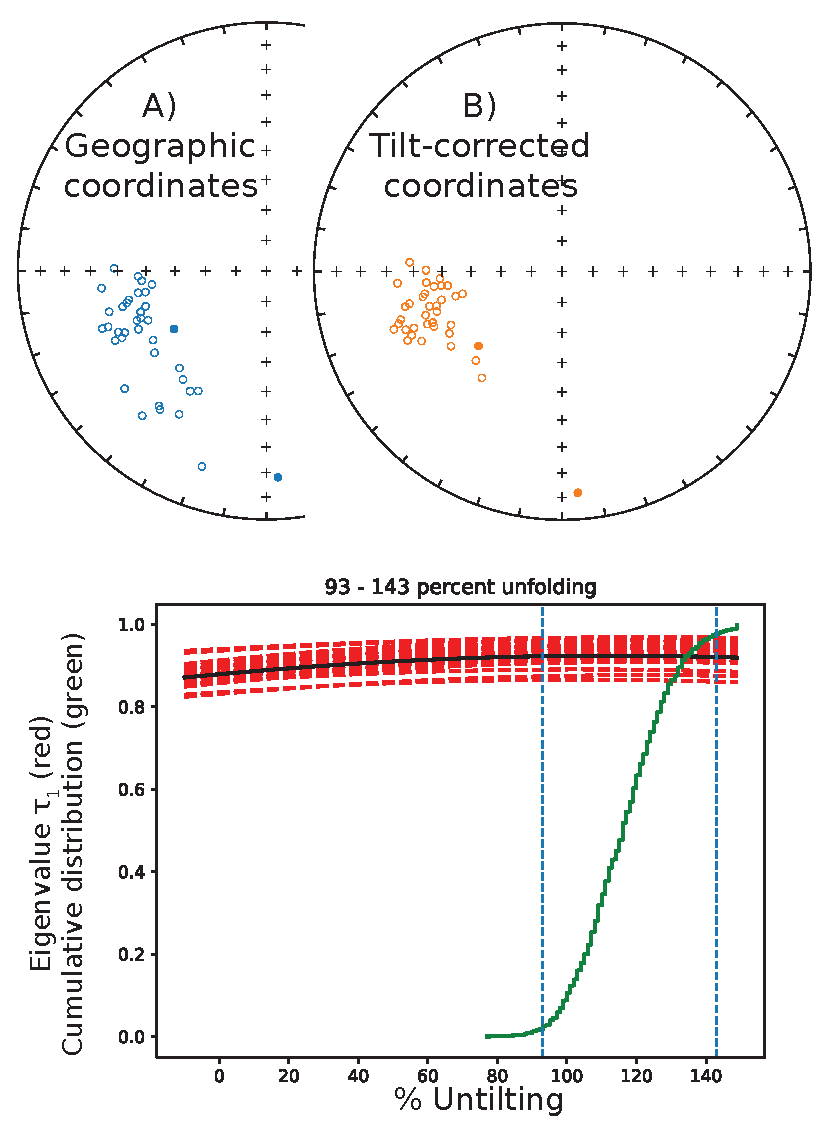
\includegraphics[width=0.5\textwidth]{SC1_fold_test.pdf}
\caption{Bootstrap paleomagnetic fold test \cite{Tauxe1994a} of the detrital remanent magnetization directions recorded by specimens from the nearly horizontal beds and moderately tilted beds at the Snake Creek tributary. Complete unfolding lies within the 95\% confidence limits of the test, consistent with the magnetization having been acquired prior to tilting.}
\label{fig:fold_test}
\end{SCfigure*}

\subsection*{Paleomagnetic reversals}

With the insights gained from the thermal demagnetization results of the Jacobsville fluvial intraclasts and the fold test (Figs. \ref{fig:intraclast_pmag} and \ref{fig:fold_test}), we next investigate the detrital remanent magnetizations for all \textit{in situ} specimens from the five stratigraphic sections (Figs. \ref{fig:Geologic_map} and \ref{fig:strat_column}). The DRM directions are plotted by stratigraphic section location in Figure \ref{fig:in_situ_pmag}. As observed in the sparser data of \citeA{Roy1978a}, there are dual polarity magnetizations (Fig. \ref{fig:strat_column}). The paleomagnetic polarity reversals are shown in stratigraphic context in Figure \ref{fig:strat_column} with specimen magnetization declinations plotted against stratigraphic heights. The record of Laurentia's paleomagnetic poles from the Proterozoic through the Phanerozoic (see compilations in \citeA{Torsvik2012a} and \citeA{Swanson-Hysell2021c}) gives a continuity of the orientation of the continent that enables the geomagnetic polarity of the directions to be interpreted. In this framework, the westerly DRM directions are normal geomagnetic polarity and the easterly DRM directions are reversed polarity (Fig. \ref{fig:in_situ_pmag}). 

At the Dover Creek section, which goes along Dover Creek and then up the waterfall of a side tributary (the Hungarian Falls side falls), numerous hematite-rich siltstone to fine sandstone layers commonly occur in association with trough cross-bedded sandstone and conglomeratic facies. These lithofacies are particularly well-exposed along a tributary waterfall to Dover Creek such that 158 samples were collected for paleomagnetic study (Fig. \ref{fig:Geologic_map}, \ref{fig:strat_column}), making this section the most densely sampled amongst all the sections. The specimen DRMs show that the geomagnetic field reversed at least nine times during deposition within the section (Fig. \ref{fig:strat_column}). 

The Natural Wall and Hammel Creek sections are in close proximity to the Dover Creek section (Fig. \ref{fig:Geologic_map}) and the unique sedimentary facies association of volcanic-clast conglomerate, red siltstone, and coarse arkosic sandstone is similar to the basal $\sim$120 meters of the section at Dover Creek (Fig. \ref{fig:strat_column}). Our sampling at these two localities is more limited due to there being poorer exposures of siltstone and fine-grained sandstone beds in these sections (Fig. \ref{fig:strat_column}). At Hammel Creek, 16 samples from two siltstone layers near the base of the section are of reversed polarity (Fig. \ref{fig:strat_column}). Near the top of the Natural Wall section, consistent normal-polarity directions are recorded by 15 samples (Fig. \ref{fig:strat_column}). 

At the Snake Creek tributary (Fig. \ref{fig:Geologic_map}), 71 specimens yielded interpretable DRMs through multiple levels along the $\sim$95-meter-thick section and all show normal-polarity directions (Figs. \ref{fig:in_situ_pmag} and \ref{fig:strat_column}). At Agate Falls (Fig. \ref{fig:Geologic_map}), clay-rich detrital mica-bearing siltstone layers occur through $\sim$30 meters of strata that are incised by the Middle Branch Ontonagon River (Fig. \ref{fig:Field_photo}). 67 total paleomagnetic samples were collected on both sides of the waterfall (Fig. \ref{fig:strat_column}). At least three geomagnetic polarity reversals occurred during deposition within the Agate Falls section (Fig. \ref{fig:strat_column}). 

\begin{figure*}[h!]
\centering
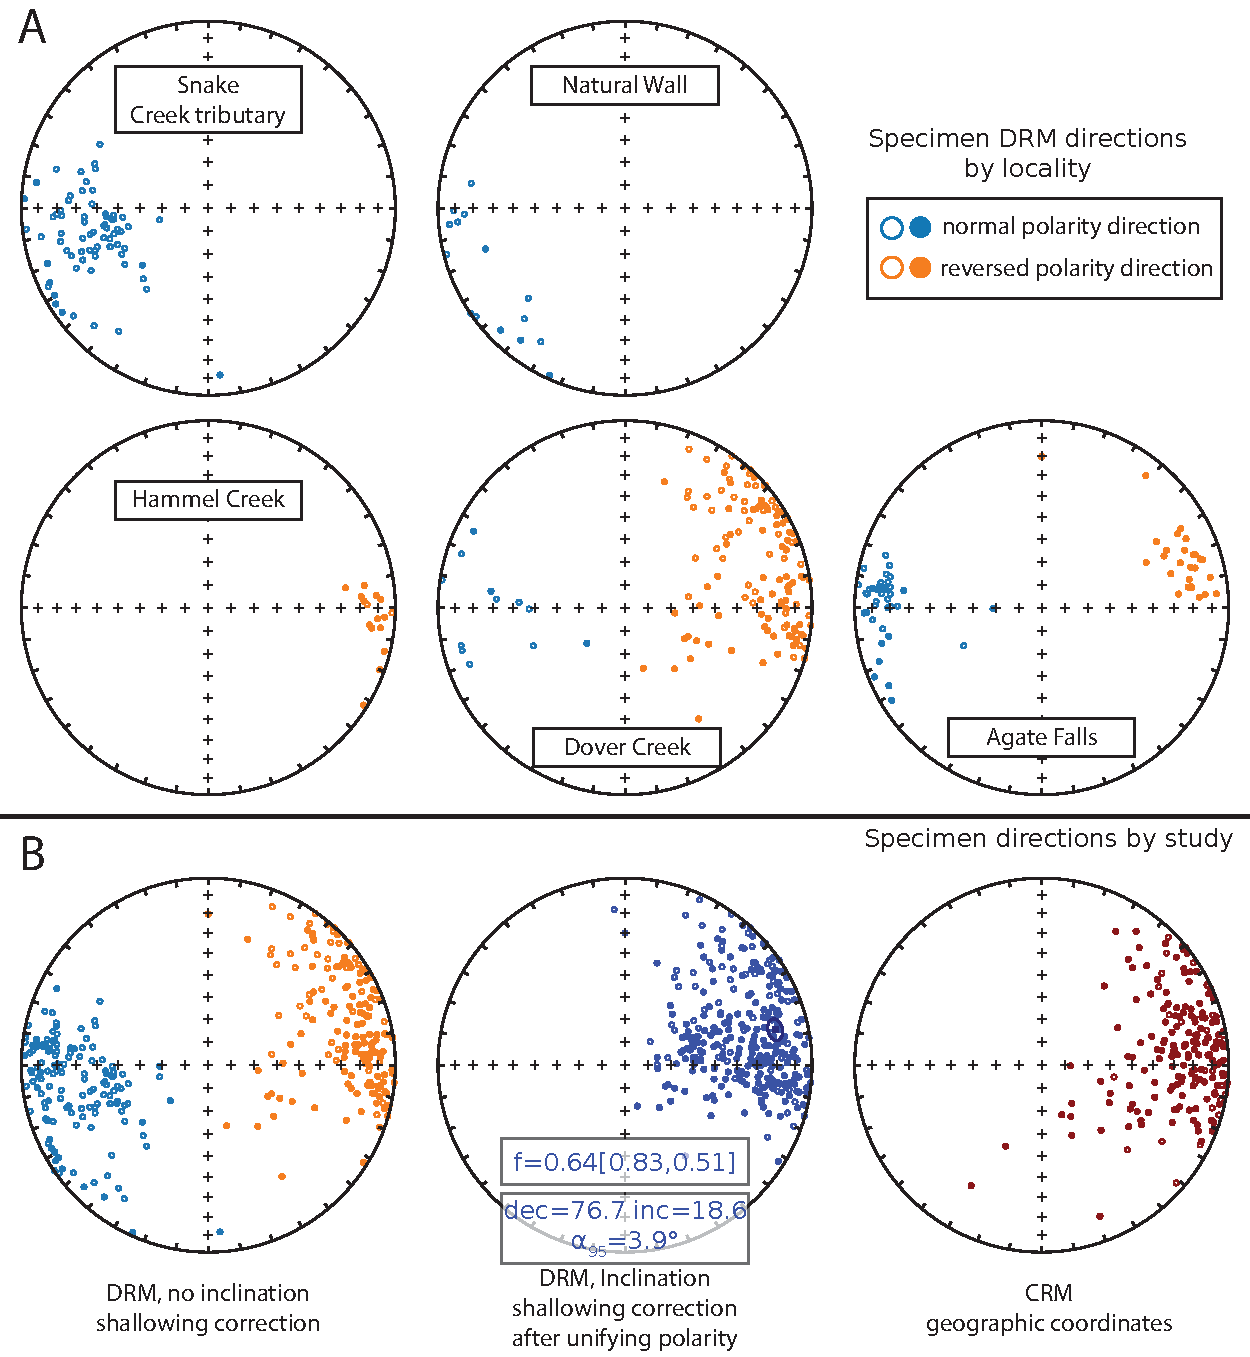
\includegraphics[width=0.8\textwidth]{in_situ_pmag.pdf}
\caption{\footnotesize (A) Specimen detrital remanence directions (DRM) plotted by locality on equal area plots. During sample collection, we optimized for vertical stratigraphic coverage such that each sample constitutes a single horizon and therefore a paleomagnetic site. Specimens from the Snake Creek tributary as a mean direction of dec=256.0\textdegree, inc=-30.5\textdegree, k=9.9, $\alpha_{95}$=5.6\textdegree, n=71; the Natural Wall section has a mean direction of dec=242.4\textdegree, inc=-6.4\textdegree, k=9.0, $\alpha_{95}$=13.5\textdegree, n=15; the Hammel Creek section has a mean direction of dec=94.1\textdegree, inc=8.7\textdegree, k=30.7, $\alpha_{95}$=6.8\textdegree, n=16; the Dover Creek section has a mean direction of dec=73.2\textdegree, inc=5.4\textdegree, k=5.6, $\alpha_{95}$=5.6\textdegree, n=138; the Agate Falls section has a mean direction of dec=83.4\textdegree, inc=13.0\textdegree, k=13.4, $\alpha_{95}$=4.9\textdegree, n=67. All reported directions are calculated in tilt-corrected coordinates and after unifying polarity. The measurement-level data are available in the MagIC database (https://earthref.org/MagIC/19780/df1b7c0c-b1cc-4e1e-b40c-2585f007178a; \textit{this link provides access to reviewers and will be updated with a final version of the link when the manuscript is accepted}). (B) Summary equal area plots at the study-level combining directions from all localities. The elongation/inclination (E/I) method \cite{Tauxe2004b} was used to estimate the amount of inclination shallowing in Jacobsville specimen DRMs after unifying the polarities (flipping the normal [blue] directions to their antipodes). Details on inclination shallowing corrections are shown in Figure \ref{fig:EI_results} with the value of $f$=0.64 used for the directions in the middle panel. All DRM directions are shown in tilt-corrected bedding coordinates. The summary plot of all specimen chemical remanence directions (CRM) are shown in geographic coordinates show well-grouped reversed-polarity directions whose directions are similar to the DRMs. }
\label{fig:in_situ_pmag}
\end{figure*}

The paleomagnetic reversal test assesses whether two directional data sets share a common mean when one of the polarity directions is flipped to its antipode. Although the occurrence of multiple geomagnetic field reversals during deposition of the Jacobsville Formation is evident (Figs. \ref{fig:strat_column} and \ref{fig:in_situ_pmag}), the limited and often discrete records of many polarity chrons are insufficient for pair-wise reversal tests within single sections (Fig. \ref{fig:strat_column}). Sedimentation within individual siltstone horizons was likely quite rapid given their deposition within fluvial floodplains potentially without sufficient time to average out secular variation within discrete siltstone intervals. We combine all normal and reversed directions from the five sections and perform a reversal test. The \citeA{McFadden1990a} reversal test results show the angle between the two mean directions (15.9\textdegree; no inclination shallowing correction) exceeds the critical angle (7.5\textdegree) (Fig. S5), thereby failing the test. This difference largely arises due to normal (west directed) directions in the Snake Creek tributary section being slightly steeper in their upward inclination. There are at least four possible explanations for this behavior: 1) the lower number of normal directions which dominantly come from the Snake Creek tributary section may not have averaged out secular variation; 2) there could have been plate motion during Jacobsville deposition with the normal polarity in the Snake Creek tributary section being acquired when Laurentia was at a slightly higher latitude; 3) there could be a bias from the reversed CRM superimposed on the normal DRM in the Snake Creek tributary specimens being incompletely removed during thermal demagnetization; 4) the geomagnetic field in the early Neoproterozoic could have been slightly different than that of more recent times in terms of the dispersion of pole position at distinct time snapshots potentially associated with changes in field intensity. Regardless, the positive intraclast conglomerate test gives confidence that the Jacobsville Formation has a primary detrital remanent magnetization that can be isolated through thermal demagnetization. This result is strengthened through the positive fold test and the broadly antipodal dual polarity data. Additionally, taking the large number of samples together from both polarities to calculate a pole increases the likelihood that the dual polarity pole has averaged out secular variation.

A total of 186 specimens yielded interpretable chemical remanence directions that are of dominantly reversed polarity. These directions are plotted by stratigraphic section location in Figure S6 and are all shown in Figure 6B. That the CRM directions are a secondary remanence component that postdate the deposition of the Jacobsville Formation is supported by the negative intraformational conglomerate test results and failure in the fold test (Figs. \ref{fig:intraclast_pmag}, S4). However, the similarity of the CRM directions (declination=96.2\textdegree, inclination=15.1\textdegree, $\alpha_{95}$=4.2\textdegree, n=186) with the primary DRM directions (declination=103.1\textdegree, inclination=13.4\textdegree, $\alpha_{95}$=3.3\textdegree, n=307, no inclination shallowing correction) indicate that growth of the secondary pigmentary hematite which carries the CRM likely occurred soon after deposition when Laurentia was in a similar paleogeographic position. 

Overall, the multiple geomagnetic field polarity reversals recorded by the Jacobsville Formation constrain that the end of the Keweenawan normal superchron \cite{Driscoll2016b} (which started ca. 1099 Ma; \citeA{Swanson-Hysell2019a}) had to have ended by the onset of Jacobsville deposition.
 
\section*{Discussion}
\subsection*{Averaging paleosecular variation and correcting for inclination shallowing}

Igneous and sedimentary rocks associated with the North American Midcontinent Rift provide a high-resolution record of the ca. 1109 to 1070 Ma Keweenawan Track which tightly constrains the apparent polar wander path for Laurentia in the late Mesoproterozoic (Fig. \ref{fig:pole_plot}; \citeA{Swanson-Hysell2019a}). However, high-quality paleogeographic constraints thereafter are sparser and more uncertain in their age until the ca. 775 Ma Gunbarrel large igneous province \cite{Harlan2003a} and subsequent ca. 775-719 Ma poles from western Laurentia extensional basins \cite{Weil2006a, Eyster2019a}. Developing a new paleomagnetic pole from the Jacobsville Formation presents an opportunity for a well-constrained early Neoproterozoic constraint on Laurentia's paleogeographic position. 

Our high-resolution thermal demagnetization successfully isolated detrital magnetization from the secondary chemical magnetization carried by pigmentary hematite that grew after deposition of the Jacobsville Formation. The scatter in the DRM directions can be interpreted to reflect variations in the geomagnetic field during the deposition of the sediments \cite{Steiner1983a, Tauxe1984a}. The multiple geomagnetic field reversals captured by specimens collected from the Dover Creek and Agate Falls sections support that a prolonged period of time is represented by the specimens given that the duration of geomagnetic polarity chrons are typically on the order of tens of Kyr to Myr timescales (Fig. \ref{fig:strat_column}). Therefore, we combine all specimen detrital remanent magnetizations to calculate a paleomagnetic pole for the Jacobsville Formation.

A challenge in interpreting detrital magnetizations is the issue of correcting for inclination shallowing \cite{King1955a, Tauxe2004b, Bilardello2016b}. Scatter of the specimen detrital remanence directions in tilt-corrected coordinates show elongation parallel to the bedding plane, consistent with them being shallowed (Fig. \ref{fig:in_situ_pmag}; \citeA{Tauxe2004b}). Such a directional distribution is due to rotation of detrital hematite grains during deposition and subsequent compaction, resulting in inclinations recorded by sedimentary rocks having shallower angles than the local field in which they are deposited. If uncorrected, shallower inclinations obtained from sedimentary rocks can result in erroneously low estimates of paleolatitudes, biasing paleogeographic reconstructions. To estimate the amount of inclination shallowing, we apply the statistical elongation/inclination (E/I) method that evaluates the deviation of the distribution of a large number ($>$100) of observed sedimentary paleomagnetic directional data with the predicted distribution given by a statistical paleosecular variation model \cite{Tauxe2004b}. Although the TK03 paleosecular variation model is based on data of relatively recent geomagnetic field variations, it has been shown to be compatible with data from the ca. 1.1 Ga lava flows of the Midcontinent Rift \cite{Tauxe2009a}. Furthermore, \citeA{Pierce2022a} showed that applying the E/I method to detrital hematite magnetizations within the ca. 1093 Ma Cut Face Creek Sandstone in the Midcontinent Rift successfully corrects the shallow paleomagnetic inclinations of the sediments to that of the North Shore Volcanic Group lava flows that bracket them. \citeA{Pierce2022a} also developed a method, that we use here, to represent uncertainties associated with the amount of inclination shallowing into sedimentary paleomagnetic pole positions which can then be summarized with an elliptical Kent distribution \cite{Kent1982a} rather than a circular Fisher distribution \cite{Fisher1953a}. 

Applying the E/I method to the Jacobsville DRM directions results in an estimate for the flattening factor ($f$ factor) of 0.64 with a 95\% uncertainty range of 0.83 to 0.51 (Figs. \ref{fig:EI_results}). The $f$ factor of 0.64 is close to the value of 0.58 which is the mean of inclination shallowing factors compiled for hematite-bearing rocks in \citeA{Pierce2022a} (building on compilations of \citeA{Bilardello2016b} and \citeA{Vaes2021a}). The Fisher mean inclination-corrected detrital remanence mean direction is dec=76.7\textdegree, inc=18.6\textdegree $\alpha_{95}$=3.9\textdegree. The Fisher mean inclination-corrected paleomagnetic pole associated with this nominal $f$ factor is Plon=183.4\textdegree E, Plat=16.9\textdegree S, A$_{95}$=3.1\textdegree. We apply the method of \citeA{Pierce2022a} to incorporate the uncertainty in the E/I estimate of the $f$ factor into the uncertainty of the paleomagnetic pole (Fig. \ref{fig:EI_results}). This uncertainty results in more uncertainty associated with paleolatitude which for the pole is along the great circle path between the mean pole position and the locality of the Jacobsville sections. Following \citeA{Pierce2022a}, the pole can be represented with a Kent distribution 95\% confidence ellipse which is: mean longitude=183.4\textdegree E, mean latitude=16.9\textdegree S, major axis longitude=255.5\textdegree E, major axis latitude=45.2\textdegree N, major axis magnitude=4.1\textdegree, minor axis longitude=108.1\textdegree E, minor axis latitude=39.9\textdegree N, minor axis magnitude=3.1\textdegree (Fig. \ref{fig:EI_results}; Table \ref{tab:Kent_means}). This pole position is close to the end of the Keweenawan Track (Fig.\ref{fig:pole_plot}) and far away from Laurentia's pole positions during the Paleozoic when there was orogenesis along Laurentia's eastern margin (Fig. S7). This pole position is consistent with the geochronology constraints on the deposition of the Jacobsville Formation and the positive paleomagnetic field tests that the detrital remanence of the Jacobsville Formation was acquired during the earliest Neoproterozoic. 


\begin{figure*}[h!]
\centering
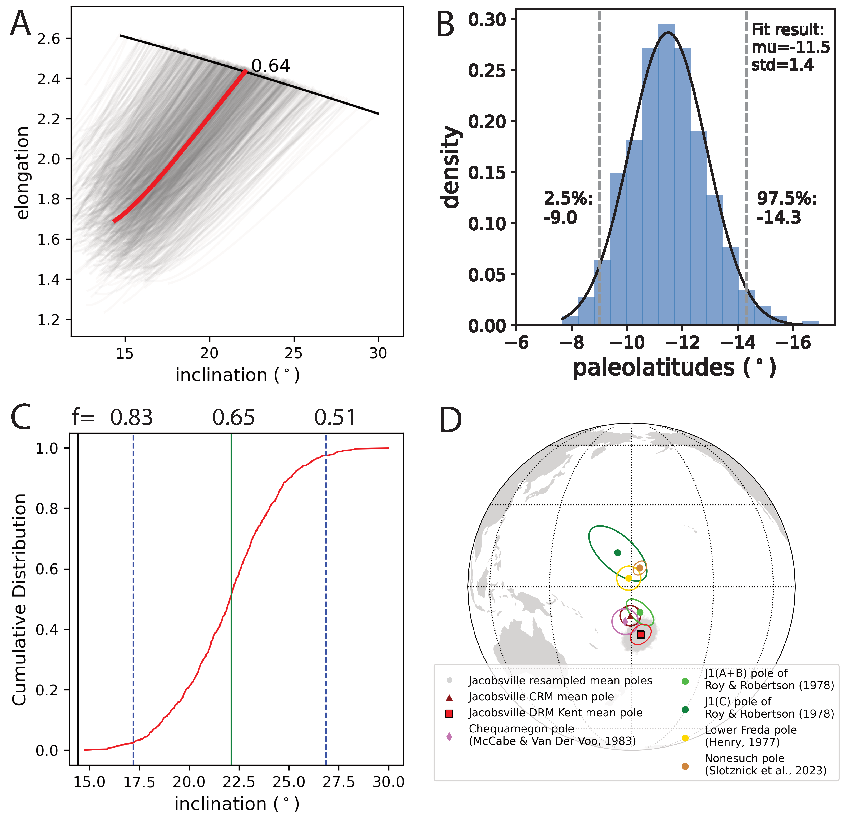
\includegraphics[width=\textwidth]{EI_results.pdf}
\caption{\scriptsize Results of the estimated amount of inclination shallowing of the detrital remanent magnetization of the Jacobsville Formation using the elongation/inclination (E/I) method \cite{Tauxe2004b}. (A) The E/I method gives an estimated flattening factor $f$=0.64 (red curve) based on where the elongation/inclination curve of the dataset intersects that predicted by the TK03 paleosecular variation model (black curve; \citeA{Tauxe2004b}). The grey lines show 1,000 bootstrap resamples of the DRM directions which provide an estimate of the uncertainty associated with the $f$ factor estimate (95\% interval from 0.83 to 0.51). (B) The distribution of the paleolatitudes resulting from the corrected inclinations of the E/I bootstrap resamples. That the distribution is drawn from a normal distribution with a mean of -11.5\textdegree\ and standard deviation of 1.4 cannot be rejected in the Kolmogorov-Smirnov test. The 95\% confidence bounds shown by dashed lines span a range of paleolatitudes that need to be incorporated into the uncertainty of the reported paleomagnetic pole. (C) The cumulative distribution of inclinations based on the E/I bootstrap results with the 95\% confidence bounds shown in terms of inclination and $f$ factor. (D) The new Kent mean inclination corrected DRM pole (red square) of the Jacobsville Formation is shown in the context of the pole calculated for the CRM (purple triangle) as well as the Jacobsville pole developed by \citeA{Roy1978a}, the Chequamegon Formation pole of \citeA{McCabe1983a}, and poles from the Oronto Group (Nonesuch Formation, \citeA{Slotznick2023a}; Freda Formation, \citeA{Henry1977a}). The mean pole position of the Kent distribution was calculated following the method of \citeA{Pierce2022a}. The close proximity between Jacobsville poles with the Chequamegon pole is consistent with their deposition being coeval. In contrast, the J1 (C) pole of \citeA{Roy1978a} developed from hematite-bearing sedimentary rocks in the Sault Ste Marie region plots in the northern hemisphere close to the Freda Formation pole. }
\label{fig:EI_results}
\end{figure*}

\begin{table}[h!]
   \caption{Kent mean paleomagnetic pole for the Jacobsville Formation} 
   \label{tab:Kent_means}
   \footnotesize
   \singlespacing
   \centering
   \begin{tabular}{p{0.8 in}p{0.8 in}p{0.8 in}p{0.8 in}p{0.8 in}p{0.8 in}}
   \hline
   pole & mean pole position (Plon/Plat) & major axis & major axis 95\% confidence angle & minor axis & minor axis 95\% confidence angle \\
   & $\gamma_{1}$ & $\gamma_{2}$ & $\zeta_{95}$ & $\gamma_{3}$ & $\eta_{95}$ \\
   \hline
   Jacobsville $E/I$ corrected & 183.4\textdegree E / 16.9\textdegree S &  255.5\textdegree E / 45.2\textdegree N & 4.1\textdegree &
   108.1\textdegree E / 39.9\textdegree N & 3.1\textdegree \\
   \hline
 \multicolumn{6}{p{5.5 in}}{Notes: The Fisher mean of the Jacobsville detrital remanence paleomagnetic pole without an inclination shallowing correction is Plon=185.5\textdegree E, Plat=14.0\textdegree S, A$_{95}$=2.7\textdegree; the Fisher mean of the Jacobsville detrital remanence paleomagnetic pole with an inclination shallowing correction of $f$=0.64 is Plon=183.4\textdegree E, Plat=16.9\textdegree S, A$_{95}$=3.1\textdegree; the Fisher mean of the Jacobsville chemical remanence paleomagnetic pole is Plon=179.6\textdegree E, Plat=10.2\textdegree S, A$_{95}$=3.6\textdegree}
   \end{tabular}
\end{table}

\citeA{Roy1978a} also studied the paleomagnetism of sedimentary rocks grouped as the Jacobsville Formation and isolated a characteristic magnetization component via alternating-field, thermal, and chemical demagnetization on a suite of Jacobsville red beds near the Keweenaw Peninsula (their area A), the town of Marquette (their area B), and Sault Ste Marie (their area C). Although least-squares principal component analyses was not a routine approach in fitting paleomagnetic directions at the time, that study had success in removing the present day local field overprint and was able to resolve dual magnetic polarities at one locality. The mean paleomagnetic pole position calculated from the interpreted primary magnetic remanence from rocks of the Keweenaw Peninsula and Marquette area (J1 A+B pole; pole longitude=183\textdegree E, pole latitude=9\textdegree S, dp=3\textdegree, dm=6\textdegree; no inclination correction; Fig. \ref{fig:EI_results}; \citeA{Roy1978a}) is in the southern hemisphere and lies close to the mean pole from this study (Fig. \ref{fig:EI_results}). However, their mean pole developed from fine- and medium-grained sandstone near Sault Ste Marie lies in the northern hemisphere with a pole latitude of 12\textdegree N (Fig. \ref{fig:EI_results}). Despite the large uncertainty ellipse associated with this mean pole position, it is distinct from the mean pole position from the Jacobsville Formation in northern Michigan. Instead, it overlaps with the Oronto Group paleomagnetic poles of the ca. 1070 Ma lower Freda Formation and the ca. 1075 Ma Nonesuch Formation (Fig. \ref{fig:EI_results}; \citeA{Henry1977a, Slotznick2023a}). As suggested by \citeA{Dubois1962a} and \citeA{Roy1978a}, these data suggest that the fluvial red beds in the Sault Ste Marie area that are often taken to be correlative to the Jacobsville Formation \cite<e.g.>{Malone2020a} are likely time equivalent to sedimentary rocks of the Oronto Group and deposited during post-rift thermal subsidence. 

Deposition of Bayfield Group sedimentary rocks in northern Wisconsin (west of the studied exposures; Fig. \ref{fig:Geologic_map}) has been hypothesized to be coeval with the Jacobsville Formation \cite{Hamblin1958a, Kalliokoski1982a, Malone2016a}. Published low precision detrital zircon U-Pb dates developed by laser ablation–inductively coupled plasma–mass spectrometry (LA-ICP-MS) dates are consistent with this interpretation with a maximum depositional age of ca. 1035 Ma for the Chequamegon Formation of the Bayfield Group \cite{Craddock2013a}. Our updated Jacobsville pole position is close to a pole developed from the Chequamegon Sandstone of the Bayfield Group (Fig. \ref{fig:EI_results}; pole longitude=177.7\textdegree E, pole latitude=12.3\textdegree S, A$_95$=4.6\textdegree; no inclination correction; \citeA{McCabe1983a}). These data are consistent with the Bayfield Group being deposited within a contiguous syn-orogenic basin with the Jacobsville Formation during the Rigolet phase of the Grenvillian orogeny. This interpretation can be evaluated with further high-precision geochronology focused on the Bayfield Group. 

\subsection*{Age of the Jacobsville Pole}

At the western edge of the Jacobsville bedrock belt in northern Michigan, the formation is in angular unconformity with Midcontinent Rift rocks that were uplifted and tilted prior to Jacobsville deposition (Fig. \ref{fig:Geologic_map}; \citeA{Hedgman1992a, Cannon1995a}). Rb-Sr thermochronologic data developed from Paleoproterozoic to Archean lithologies that were exhumed along the Marenisco Fault along with Midcontinent Rift strata in this region indicate that this uplift occurred ca. 1050 Ma associated with the Ottawan phase of the Grenvillian orogeny \citeA{Cannon1993a}. Field observations reveal erosional contacts and development of paleosols between the Jacobsville Formation and underlying Midcontinent Rift volcanic rocks at the Sturgeon River within the bedrock belt \cite{Hamblin1958a, Zbinden1988a}. Seismic reflection data beneath Lake Superior have been also been interpreted to indicate that the Jacobsville Formation lies in angular unconformity atop sedimentary rocks of the Oronto Group \cite{Cannon1989a}. This context requires that there was ca. 1050 Ma contractional deformation of Midcontinent Rift strata, erosion of these tilted strata, and renewed subsidence prior to the onset of Jacobsville deposition atop them.

Maximum depositional detrital zircon dates are consistent with this history and provide additional constraints. \citeA{Hodgin2022a} applied tandem dating where the young population emerging from a large number of low-precision LA-ICP-MS dates are followed by high-precision CA-ID-TIMS analysis. This approach has the advantage of combining the high number of low-precision analyses that can be acquired through LA-ICP-MS with dates developed through CA-ID-TIMS where the deleterious effects of Pb-loss can be mitigated, and more accurate and precise dates can be obtained. These data reveal the youngest zircon at Sandstone Creek near the Keweenaw Fault (Figure \ref{fig:Geologic_map}) to have a date of 992.51$\pm$0.64 Ma (2$\sigma$ analytical uncertainty) and the youngest zircon at Agate Falls (Figure \ref{fig:Geologic_map}) a date of 1003.21 $\pm$ 2.23 Ma (2$\sigma$). These dates are consistent with the age of syntectonic magmatism in the Grenville orogen associated with the Rigolet phase of the orogeny \cite<e.g.>{Bussy1995a, Turlin2019a, Jannin2018a} which is a potential source for the grains. Overall, these dates constrain a maximum depositional age of the Jacobsville Formation in the earliest Neoproterozoic. 

While there has been recent success in applying tandem detrital zircon data to obtain maximum depositional ages that are close to true depositional ages \cite{Karlstrom2020a}, the possibility exists that deposition could significantly postdate the youngest dated detrital zircon. A firm minimum depositional age on the age of the Jacobsville is that it is unconformably overlain by the Cambrian Munising Formation whose base was deposited ca. 501 to 497 Ma during the Dresbachian Stage (the Guzhangian Stage in the modern Cambrian time scale) \cite{Hamblin1958a, Haddox1990a}. This unconformity is erosional as it truncates Jacobsville strata and intraformational clastic dikes and can have slight angularity \cite{Hamblin1958a, Haddox1990a}. That the Jacobsville Formation is older than the Munising Formation lends tighter constraints than the Cambrian age itself given the evidence discussed above that Jacobsville deposition was syn-orogenic. The only candidate for such orogenesis is the ca. 1010-980 Ma Rigolet phase of the Grenvillian orogeny given that subsequent Paleozoic orogenesis (e.g. the Ordovician Taconic and Carboniferous Alleghanian orogenies) post-dates deposition of the Munising Formation.

That the Jacobsville Formation is folded in the footwall of the Keweenaw fault, beneath the older Midcontinent Rift volcanic rocks in the hanging wall, provides another opportunity to develop a minimum depositional age. Seeking to obtain such a constraint, \citeA{Hodgin2022a} targeted calcite within a Keweenaw Fault breccia that cross-cuts a dense network of zeolite veins and slickenslides that yielded a U-Pb date of 985.5$\pm$35.8 Ma (2$\sigma$). While this calcite date has large analytical uncertainty, it indicates that the fault breccia developed associated with the Grenvillian orogeny and it overlaps with the ca. 1010-980 Ma ages of metamorphism associated with the Rigolet phase of the orogeny \cite{Swanson-Hysell2023a}. It is during this ca. 1010-980 Ma Rigolet phase of the orogeny that the Grenville Front developed \cite{Rivers2008a} which indicates that this was a time period when contractional deformation associated with the orogeny was propagating into the Superior craton. Together, the detrital zircon, sedimentology, and the fault calcite dates are consistent with the Jacobsville Formation being deposited in a syn-orogenic Grenville backbulge basin and subsequently deformed as contraction associated with the Rigolet phase of the Grenville orogeny propagated into the interior of Laurentia. 

Previously, some researchers have interpreted there to have been large-scale regional contractional deformation during the Alleghanian orogeny in the Paleozoic leading to reactivation of reverse faults including the Keweenaw Fault \cite{Craddock2017a}. While the Keweenaw Fault is defined quite broadly in \citeA{Craddock2017a}, the evidence put forward that is relevant to the segment in this study region are: 1) an interpreted post-Grenvillian orogeny age for the Jacobsville Formation which would require that the deformation of the formation was associated with subsequent orogenesis; and 2) deformation within two $<$1.5 km diameter outliers of Paleozoic sedimentary rocks that overlie the Jacobsville (Limestone Mountain in Figure \ref{fig:Geologic_map}). The data used to argue for a post-Grenvillian depositional age of the Jacobsville Formation were the low-precision LA-ICP-MS detrital zircon dates of \citeA{Malone2016a} that have now been superseded by the tandem dates of \citeA{Hodgin2022a}. These dates are consistent with syn-Grenvillian deposition. This progress leaves the tilted and/or brecciated Paleozoic strata in the small exposed Paleozoic outliers of the 1.5 x 1 km Limestone Mountain and the neighboring 0.5 x 0.3 km Sherman Hill as evidence of Paleozoic deformation: interpreted to be Paleozoic orogenesis by \citeA{Hamblin1958a, Craddock2017a} and suggested to be an impact structure by others \cite{Milstein1987a}. The impact origin interpretation builds on previous interpretations of the structure as being cryptovolcanic \cite{Cannon1981a}--a common interpretation for structures that have subsequently been recognized as impact related. The tilt and brecciation of these outliers contrasts with widespread flat-laying Paleozoic sedimentary rocks that overlie the reverse faults that underwent contractional deformation associated with rift inversion in Minnesota \cite{Jirsa2011a}. These strata constrain Paleozoic deformation to have been relatively minor on the scale of 10s of meters rather than the kilometers of uplift associated with the rift inversion along these reverse faults \cite{Boerboom2018a}. Clumped isotope temperatures of $\sim$50\textdegree C from the Neoproterozoic fault calcite, also developed by \citeA{Hodgin2022a}, reveal that the Keweenaw fault zone was within a couple kilometers of the surface at the time of late Mesoproterozoic to early Neoproterozoic calcite precipitation. These data are inconsistent with major Paleozoic uplift and support the interpretation that the majority of contractional inversion along the Keweenaw Fault occurred during the Rigolet Stage of the orogeny. 

Our new paleomagnetic data provides additional insights into the timing of Jacobsville deformation in the early Neoproterozoic. At the Snake Creek tributary section which is folded against the Keweenaw Fault (Figure \ref{fig:Geologic_map}, \ref{fig:strat_column}), the chemical remanence directions held by pigmentary hematite fail a fold test (Figure S4), indicating that the pigmentary hematite holding the remanence grew after deformation of the strata. The mean pole position of the chemical remanent magnetization at the Snake Creek tributary section overlaps with paleomagnetic poles of the Grenville Loop that have been assigned exhumation ages of ca. 970-960 Ma (Figure S7; \citeA{Brown2012a}). This chemical remanence pole position and the mean Jacobsville detrital remanence pole position are both far away from Laurentia's pole positions at the times of Paleozoic orogenesis or any younger time in the Phanerozoic (Figure S7). This result indicates that the majority of the tilting of the Jacobsville in the footwall of the Keweenaw Fault could not have occurred during Paleozoic orogenesis such as the Alleghanian orogeny as the chemical remanent magnetization would then be expected to record a direction aligned with the Phanerozoic pole path. Instead, the Rigolet phase of Grenvillian orogeny, which ended by ca. 980 Ma, is the only feasible orogenic interval that could have tilted these strata. This result constrains the Jacobsville Formation in the studied outcrop belt to have been deposited prior to ca. 980 Ma. While Paleozoic reactivation could have occurred, and there could be deformation of that age elsewhere such as at Limestone Mountain, deformation at this time on the Keweenaw Fault would have been relatively minor compared to that in the early Neoproterozoic.

In conclusion, our paleomagnetic data and existing chronological data combined with the geological constraints are most consistent with the interpretation that the Jacobsville Formation within the studied bedrock belt was deposited in a syn-orogenic basin associated with the Rigolet Phase of the Grenvillian orogeny. This syn-orogenic basinal setting, which is consistent with the sedimentology of the formation (Fig. \ref{fig:strat_column}), provides a mechanism for developing accommodation space. The total duration of deposition of the Jacobsville is uncertain with these constraints alone particularly given the low precision on the 985.5$\pm$35.8 Ma calcite date. However, data from the Grenville orogen itself constrain the end of the Rigolet phase to be ca. 980 Ma \cite{Swanson-Hysell2023a}. As the studied sections proximal to the Keweenaw Fault were deformed in its footwall during this phase of contractional deformation, it is reasonable to interpret deposition as occurring before the ca. 980 Ma cessation of Grenvillian orogenesis. Taken together, we consider the best nominal age constraint for the depositional age of the Jacobsville Formation to pair with the Jacobsville paleomagnetic pole position to be ca. 990 Ma as the Rigolet phase of the orogeny was ongoing. While deposition within peripheral foreland basins typically lasts between 10 and 50 million years \cite{Woodcock2004a}, the backbulge depocenter may not be as stable or long-lived. Given the available chronometric constraints from the Jacobsville Formation, the Keweenaw Fault and the Rigolet phase in the Grenville orogen, deposition of the Jacobsville can be considered to have occurred within the 1000 to 980 Ma time interval.

\subsection*{Slowdown of Laurentia's plate motion due to the Grenvillian orogeny}

The ca. 1109-1070 Ma Keweenawan Track constrains rapid motion of Laurentia from high latitudes toward the equator (Fig. \ref{fig:paleogeography}; \citeA{Davis1997a, Swanson-Hysell2019a}). Apparent polar wander path inversion results are consistent with the pole path being dominated by plate tectonic motion that could have reached a rate of 30 cm/yr (95\% interval of 27-34 cm/yr; one Euler pole scenario; \citeA{Swanson-Hysell2019a, Rose2022a}); even faster than the rate of Indian plate motion during the closure of the Neotethys Ocean \cite{Hinsbergen2022a, Jagoutz2015a}. Laurentia's rapid motion preceded and coincided with the onset of the collisional Grenvillian orogeny. In contrast to the rapid changes in pole position associated with the Keweenawan Track, the relatively close proximity between the ca. 990 Ma Jacobsville pole and ca. 1085 to 1070 Ma poles indicate that Laurentia's motion significantly slowed following the onset of the Grenvillian orogeny (Figs. \ref{fig:pole_plot} and \ref{fig:paleogeography}). Lacking chronostratigraphic constraints, previous treatments have assigned an age to the Jacobsville pole of \citeA{Roy1978a} through extrapolation of the motion of the Keweenawan Track \cite<e.g.>{Li2008a}. With the improved age constraints of \citeA{Hodgin2022a} and our new paleomagnetic pole, we can instead constrain that Laurentia's motion decreased by an order of magnitude. Incorporating temporal and spatial uncertainty on the poles gives APWP rate of $\sim$3.2 cm/yr (95\% interval from 2.5 cm/yr to 4.3 cm/yr; Fig. S8) between ca. 1070 to 990 Ma.  

\begin{figure*}[h!]
\centering
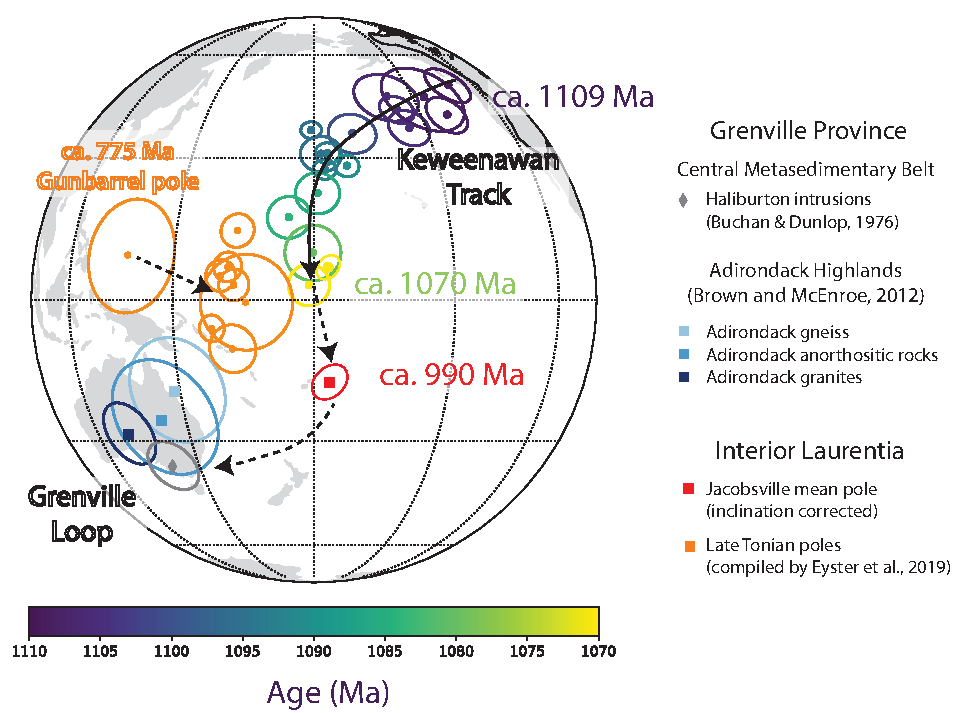
\includegraphics[width=\textwidth]{Jacobsville_pole_plot.pdf}
\caption{The inclination-corrected Jacobsville Formation detrital remanent magnetization mean pole position with its Kent uncertainty ellipse is plotted in context of the ca. 1109-1070 Ma Keweenawan Track (poles color-coded by age shown in the colorbar), selected poles from the Grenville Province, and late Tonian poles of Laurentia as compiled by \citeA{Eyster2019a} (orange colored poles). The southerly pole position of the ca. 990 Ma Jacobsville Formation indicates that the study area was crossing the equator in the late Mesoproterozoic to early Neoproterozoic. Given the large arc distance between the ca. 990 Ma Jacobsville pole and the poles of the Grenville loop, such as those of the the Haliburton intrusions, we suggest that estimates of their age as $>$1000 Ma \cite{Warnock2000a, Halls2015b, Evans2021b} are likely too old. The solid curve with arrow represents a continuous path of the Keweenawan Track, the dashed curves with arrow represent inferred apparent polar wander in the early Neoproterozoic based on data developed and compiled in this study and by \citeA{Eyster2019a}. The pole compilation used in this figure is included as Table S1. }
\label{fig:pole_plot}
\end{figure*}

This slowdown in plate motion is geodynamically consistent with the onset of Grenvillian orogenesis. The earliest records of orogenesis on the leading margin of Laurentia occur ca. 1090 Ma with estimates of peak orogenesis associated with the Ottawan stage of the orogeny occurring ca. 1050 Ma \cite{Rivers2012a, Swanson-Hysell2023a}. Inversions of the Keweenawan Track that incorporate multiple tectonic Euler poles indicate a slowdown from rates exceeding 20 cm/yr prior to 1095 Ma to rates below 20 cm/yr after 1095 Ma \cite{Swanson-Hysell2019a, Rose2022a}. This initial slowdown could be associated with soft collision as contractional deformation initiated on the leading edge of Laurentia \cite{Staal2020a}. Continued contractional collision led to substantially thickened crust recorded by granulite-facies metamorphic rocks by the time of peak Ottawan phase metamorphism ca. 1050 Ma \cite{Rivers2012a}. The large slowdown in plate speed as now constrained by the Jacobsville paleomagnetic pole is associated with this progression to hard continent-continent collision involving increased crustal thickening and progressive transmission of contractional stress that eventually progressed into the interior of Laurentia \cite{Cannon1994a}.

Laurentia's rapid motion was associated with closure of the Unimos Ocean and is consistent with it being on the lower plate that subducted under a conjugate continent (e.g. Amazonia) that collided on its margin (\citeA{Swanson-Hysell2023a}; Fig. \ref{fig:paleogeography}). The Jacobsville paleomagnetic pole constrains this motion to have slowed as orogeny progressed to be a large-scale continent-continent collision. As a result, Laurentia maintained a low-latitude position throughout the duration of the Grenvillian orogeny which sutured continents together into the supercontinent Rodinia (Fig. \ref{fig:paleogeography}). 

\subsection*{Implications for the age of the Grenville Loop}

Given that the age and pole position of the Jacobsville Formation had been uncertain and lacking other constraints from sedimentary or volcanic rocks, reconstruction of the paleogeography of Laurentia in the early Neoproterozoic has been reliant on paleomagnetic poles developed from metamorphic rocks within the Grenville Province \cite<e.g.>{Weil1998a}. As is shown in Figure \ref{fig:pole_plot}, paleomagnetic poles of the Grenville Loop plot near Australia in present-day coordinates; forming arc distances ranging from $\sim$35\textdegree\ to more than 50\textdegree\ away from poles at the end of the ca. 1110 to 1070 Ma Keweenawan Track (Fig. \ref{fig:pole_plot}). Determining ages associated with the Grenville Loop poles is crucial for constraining the motion of Laurentia at this time and the configuration between Laurentia and hypothesized conjugate continents such as Baltica within Rodinia \cite{Cawood2017a, Gong2018a, Swanson-Hysell2021c}.

\begin{figure*}[h!]
\centering
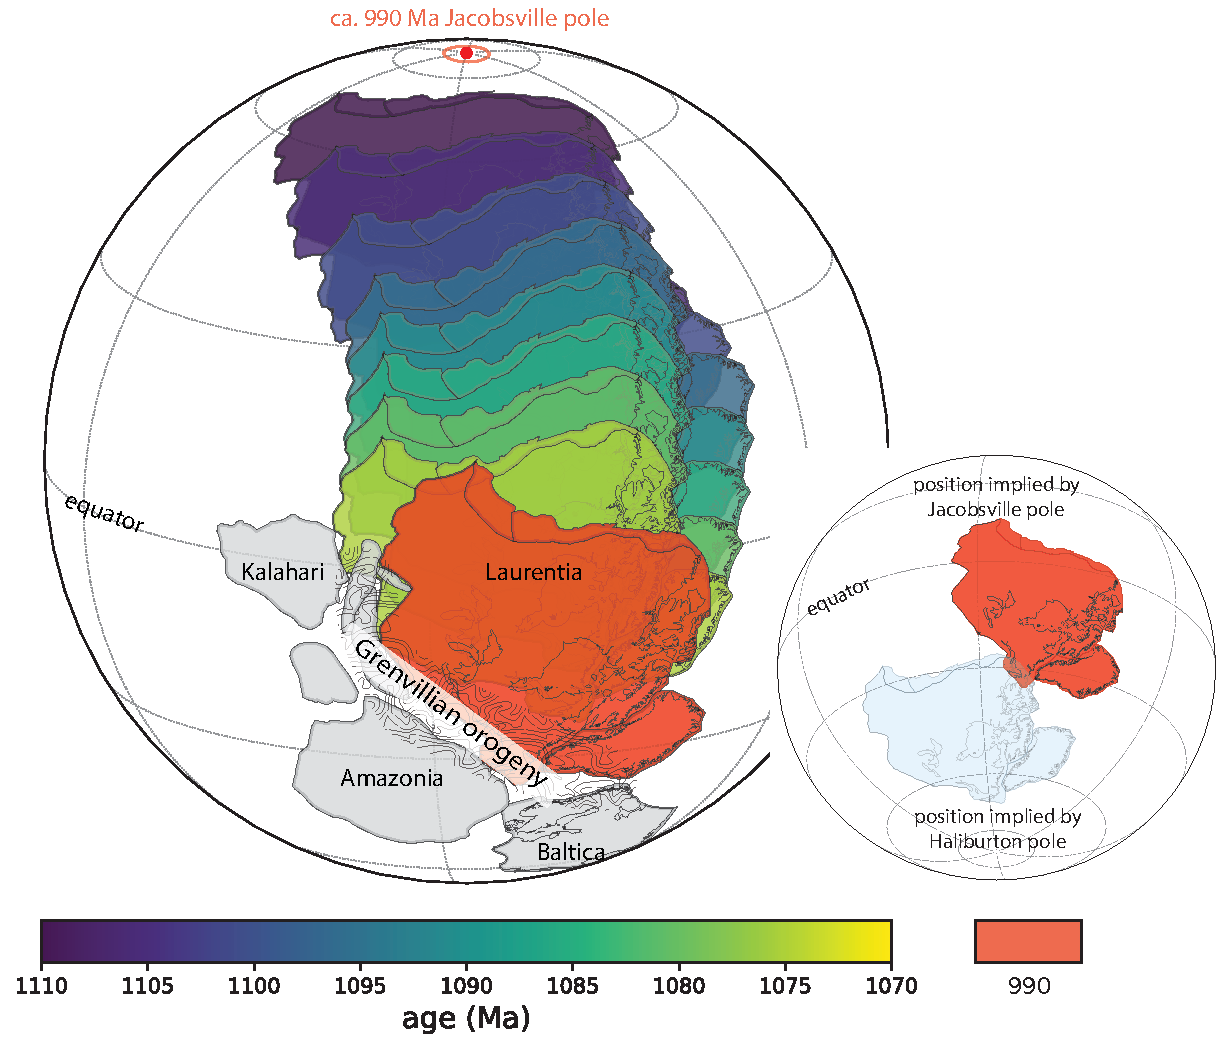
\includegraphics[width=0.8\textwidth]{Jacobsville_paleogeography.pdf}
\caption{Paleogeographic position of Laurentia through the late Mesoproterozoic to early Neoproterozoic. The color-coded reconstructions show snapshots of Laurentia's position and orientation at 5 Myr intervals from 1110 to 1075 Ma. These reconstructions implement the two-stage tectonic Euler pole rotation inversion of \citeA{Swanson-Hysell2019a}. The paleogeographic snapshot colored in red shows the position and orientation of Laurentia ca. 990 Ma as constrained by the Jacobsville paleomagnetic pole developed in this study. Interpreted positions of Laurentia's conjugate continents along its margin are shown in grey. This reconstruction shows that while Laurentia experienced rapid latitudinal changes through the Keweenawan Track that its motion was much slower between ca. 1075 and 990 Ma as the Grenvillian orogeny progressed. The paleogeographic positions of conjugate continents to Laurentia long the Grenville margin in the reconstructions follow the interpretation of \citeA{Swanson-Hysell2023a}. The inset figure compares Laurentia's position predicted by the new Jacobsville paleomagnetic pole (red) and that constrained by the Haliburton intrusions of the Grenvillian orogeny (light blue) which has been assigned an age of 1015 Ma \cite{Warnock2000a}). We suggest that this and other Grenville loop poles are younger and that Laurentia traveled from low latitudes toward higher latitudes following ca. 990 Ma while the Grenville orogen was slowly cooling and exhuming.}
\label{fig:paleogeography}
\end{figure*}

In contrast to rocks of the Midcontinent Rift where magnetizations can be confidently assigned to be the same age as the crystallization ages of the rocks \cite<e.g.>{Davis1997a,Fairchild2017a,Swanson-Hysell2019a}, rocks of the Grenville orogen experienced up to granulite facies metamorphism (temperatures $>$900\textdegree C; \citeA<e.g.>{Shinevar2021a, Metzger2021a}) and acquired magnetic remanence during subsequent exhumation \cite{McWilliams1975a, Dunlop1985a, Dodson1985a}. During slow post-orogenic exhumation (1-3\textdegree C/Myr; \citeA<e.g.>{Rivers2023a}), magnetic minerals acquired remanence by cooling through an extended temperature range over millions to tens of millions of years \cite{Pullaiah1975a, Dodson1980a} or by crystallizing through exsolution \cite{McEnroe2007a}. Determining the age of magnetization in such rocks requires reconstructing cooling histories using isotopic thermochronometers which experience radioisotopic accumulation on mineral-specific closure of elemental diffusion \cite{Dodson1973a, Dodson1985a}. 

Based on the interpretation that blocking of magnetic remanence of the magnetite-bearing Haliburton intrusions of the Grenville Central Metamorphic Belt occurred during relatively narrow temperature ranges close to the Curie temperature of magnetite (i.e. 580\textdegree C), \citeA{Warnock2000a} considered that the timing of remanence acquisition during cooling of the intrusions is bracketed between U-Pb titanite and $^{40}$Ar/$^{39}$Ar hornblende dates. As a result, that study interpreted the age associated with the Haliburton paleomagnetic pole to be ca. 1015 Ma. This age has been assigned to the pole in subsequent compilations \cite<e.g.>{Evans2021a}. In the central Adirondack Highlands of the Grenville orogen, magnetite-bearing granitic rocks and anorthositic rocks record pole positions that overlap with the Haliburton pole while their ages have been interpreted by \citeA{Brown2012a} to be ca. 990-970 Ma, based on U-Pb and $^{40}$Ar/$^{39}$Ar thermochronology data developed by \citeA{Mezger1991a}. The ca. 990 Ma Jacobsville pole position is both distinct from the Grenville Loop poles and is consistent with a slowdown of Laurentia's plate motion associated with the Grenvillian orogeny (Fig. \ref{fig:pole_plot}). If ages that have been assigned to Grenville Loop poles are taken at face value, those poles represent the position of Laurentia both before and after the position constrained by the ca. 990 Ma Jacobsville pole. Such an interpretation would imply either rapid plate tectonic motion of Laurentia coeval with the Rigolet phase of the Grenvillian orogeny or rapid oscillatory true polar wander \cite<e.g.>{Evans2003a}. A more straightforward alternative model that could explain the distinct pole positions between the Jacobsville pole and the Grenville Loop poles is that the poles from the Grenville orogen are younger than currently interpreted. Instead of having acquired remanence during the orogeny, the Grenville rocks could have acquired magnetic remanence during protracted exhumation that followed the ca. 980 Ma cessation of contractional deformation associated with the Rigolet stage of the orogeny. In this scenario, the migration of Rodinia to the higher latitude position represented by the Grenville loop poles would have occurred further into the Neoproterozoic after the Grenvillian orogeny had ceased.  

While numerous paleomagnetic data sets have been developed from rocks of the Grenville Province, few are paired with well-calibrated, high-precision thermochronology data. Recent data sets, such as new apatite U-Pb dates of 923$\pm$14 Ma (2$\sigma$ analytical uncertainty) from the Wilberforce pyroxenite \cite{Paul2021a}, give tantalizing hints that temperatures that blocked magnetizations in portions of the orogen were achieved later than the ages assigned to paleomagnetic poles would suggest as U-Pb apatite closure temperatures are close to magnetite blocking temperatures (ca. 360-570\textdegree C; \citeA{Cherniak1991a}). To test the hypothesis that the Grenville Loop is younger than in previous interpretations, geochronology studies are needed to exploit the resolving power of high-precision whole grain analytical methods (i.e. ID-TIMS) and high-spatial-resolution in-situ methods (e.g. laser ablation depth profiling; \citeA{Chew2021a}) for reconstructing the cooling rate and time-temperature history of the Grenville Province. Testing this hypothesis is critical for reconstructions of the paleogeography of Rodinia in the early Neoproterozoic. 

\section*{Conclusion}

The magnetization of hematite-bearing fine-grained siliciclastic sedimentary rocks from the Jacobsville Formation can be shown to be detrital and primary through positive intraformational conglomerate and fold tests. We use these data to develop a new inclination-corrected paleomagnetic pole that can be constrained with recently published radiometric age constraints from \citeA{Hodgin2022a} to be ca. 990 Ma. This high-quality pole is a crucial addition to Laurentia's apparent polar wander path in the earliest Neoproterozoic. Its position indicates that Laurentia's plate motion significantly slowed during Grenvillian collisional orogenesis. The new pole establishes a well-calibrated constraint for the position of the supercontinent Rodinia in early Neoproterozoic with Laurentia being at the center. The Jacobsville pole implies that ages associated with the paleomagnetic poles recorded by metamorphic rocks of the Grenville Province are likely younger than in current interpretations. Further paired studies of high-quality paleomagnetism and high-precision thermochronology are needed to illuminate Rodinia's motion and configuration in the early Neoproterozoic. 

\section*{Data Availability}
Paleomagnetic data associated with this study are available within the MagIC database (\url{10.7288/V4/MAGIC/19780}) and all data are within a Github repository associated with this work (\url{https://github.com/Swanson-Hysell-Group/Jacobsville}) that is also archived on Zenodo (\url{https://doi.org/XXX}; \textit{will be archived in Zenodo upon acceptance}). This repository also contains Python code that implements all of the calculations, visualizations and statistical tests discussed herein. 

\section*{acknowledgments}
Project research was funded by NSF CAREER grant EAR-1847277. Jim DeGraff provided helpful guidance in identifying exposures of the Jacobsville Formation. We gratefully acknowledge the Michigan Department of Natural Resources for sampling permitting. We thank Tim Lyons for additional private land access. We thank Madeline Swanson-Hysell for her assistance in the field. We thank David Malone, Douglas Elmore, and two anonymous reviewers for their helpful reviews. 

\section{Supporting Information}

\include{chap4}


\bibliography{references}
\printbibliography

% \appendix
% \chapter{More Monticello Candidates}

\end{document}